% Options for packages loaded elsewhere
\PassOptionsToPackage{unicode}{hyperref}
\PassOptionsToPackage{hyphens}{url}
%
\documentclass[
]{book}
\usepackage{amsmath,amssymb}
\usepackage{iftex}
\ifPDFTeX
  \usepackage[T1]{fontenc}
  \usepackage[utf8]{inputenc}
  \usepackage{textcomp} % provide euro and other symbols
\else % if luatex or xetex
  \usepackage{unicode-math} % this also loads fontspec
  \defaultfontfeatures{Scale=MatchLowercase}
  \defaultfontfeatures[\rmfamily]{Ligatures=TeX,Scale=1}
\fi
\usepackage{lmodern}
\ifPDFTeX\else
  % xetex/luatex font selection
\fi
% Use upquote if available, for straight quotes in verbatim environments
\IfFileExists{upquote.sty}{\usepackage{upquote}}{}
\IfFileExists{microtype.sty}{% use microtype if available
  \usepackage[]{microtype}
  \UseMicrotypeSet[protrusion]{basicmath} % disable protrusion for tt fonts
}{}
\makeatletter
\@ifundefined{KOMAClassName}{% if non-KOMA class
  \IfFileExists{parskip.sty}{%
    \usepackage{parskip}
  }{% else
    \setlength{\parindent}{0pt}
    \setlength{\parskip}{6pt plus 2pt minus 1pt}}
}{% if KOMA class
  \KOMAoptions{parskip=half}}
\makeatother
\usepackage{xcolor}
\usepackage{color}
\usepackage{fancyvrb}
\newcommand{\VerbBar}{|}
\newcommand{\VERB}{\Verb[commandchars=\\\{\}]}
\DefineVerbatimEnvironment{Highlighting}{Verbatim}{commandchars=\\\{\}}
% Add ',fontsize=\small' for more characters per line
\usepackage{framed}
\definecolor{shadecolor}{RGB}{248,248,248}
\newenvironment{Shaded}{\begin{snugshade}}{\end{snugshade}}
\newcommand{\AlertTok}[1]{\textcolor[rgb]{0.94,0.16,0.16}{#1}}
\newcommand{\AnnotationTok}[1]{\textcolor[rgb]{0.56,0.35,0.01}{\textbf{\textit{#1}}}}
\newcommand{\AttributeTok}[1]{\textcolor[rgb]{0.13,0.29,0.53}{#1}}
\newcommand{\BaseNTok}[1]{\textcolor[rgb]{0.00,0.00,0.81}{#1}}
\newcommand{\BuiltInTok}[1]{#1}
\newcommand{\CharTok}[1]{\textcolor[rgb]{0.31,0.60,0.02}{#1}}
\newcommand{\CommentTok}[1]{\textcolor[rgb]{0.56,0.35,0.01}{\textit{#1}}}
\newcommand{\CommentVarTok}[1]{\textcolor[rgb]{0.56,0.35,0.01}{\textbf{\textit{#1}}}}
\newcommand{\ConstantTok}[1]{\textcolor[rgb]{0.56,0.35,0.01}{#1}}
\newcommand{\ControlFlowTok}[1]{\textcolor[rgb]{0.13,0.29,0.53}{\textbf{#1}}}
\newcommand{\DataTypeTok}[1]{\textcolor[rgb]{0.13,0.29,0.53}{#1}}
\newcommand{\DecValTok}[1]{\textcolor[rgb]{0.00,0.00,0.81}{#1}}
\newcommand{\DocumentationTok}[1]{\textcolor[rgb]{0.56,0.35,0.01}{\textbf{\textit{#1}}}}
\newcommand{\ErrorTok}[1]{\textcolor[rgb]{0.64,0.00,0.00}{\textbf{#1}}}
\newcommand{\ExtensionTok}[1]{#1}
\newcommand{\FloatTok}[1]{\textcolor[rgb]{0.00,0.00,0.81}{#1}}
\newcommand{\FunctionTok}[1]{\textcolor[rgb]{0.13,0.29,0.53}{\textbf{#1}}}
\newcommand{\ImportTok}[1]{#1}
\newcommand{\InformationTok}[1]{\textcolor[rgb]{0.56,0.35,0.01}{\textbf{\textit{#1}}}}
\newcommand{\KeywordTok}[1]{\textcolor[rgb]{0.13,0.29,0.53}{\textbf{#1}}}
\newcommand{\NormalTok}[1]{#1}
\newcommand{\OperatorTok}[1]{\textcolor[rgb]{0.81,0.36,0.00}{\textbf{#1}}}
\newcommand{\OtherTok}[1]{\textcolor[rgb]{0.56,0.35,0.01}{#1}}
\newcommand{\PreprocessorTok}[1]{\textcolor[rgb]{0.56,0.35,0.01}{\textit{#1}}}
\newcommand{\RegionMarkerTok}[1]{#1}
\newcommand{\SpecialCharTok}[1]{\textcolor[rgb]{0.81,0.36,0.00}{\textbf{#1}}}
\newcommand{\SpecialStringTok}[1]{\textcolor[rgb]{0.31,0.60,0.02}{#1}}
\newcommand{\StringTok}[1]{\textcolor[rgb]{0.31,0.60,0.02}{#1}}
\newcommand{\VariableTok}[1]{\textcolor[rgb]{0.00,0.00,0.00}{#1}}
\newcommand{\VerbatimStringTok}[1]{\textcolor[rgb]{0.31,0.60,0.02}{#1}}
\newcommand{\WarningTok}[1]{\textcolor[rgb]{0.56,0.35,0.01}{\textbf{\textit{#1}}}}
\usepackage{longtable,booktabs,array}
\usepackage{calc} % for calculating minipage widths
% Correct order of tables after \paragraph or \subparagraph
\usepackage{etoolbox}
\makeatletter
\patchcmd\longtable{\par}{\if@noskipsec\mbox{}\fi\par}{}{}
\makeatother
% Allow footnotes in longtable head/foot
\IfFileExists{footnotehyper.sty}{\usepackage{footnotehyper}}{\usepackage{footnote}}
\makesavenoteenv{longtable}
\usepackage{graphicx}
\makeatletter
\def\maxwidth{\ifdim\Gin@nat@width>\linewidth\linewidth\else\Gin@nat@width\fi}
\def\maxheight{\ifdim\Gin@nat@height>\textheight\textheight\else\Gin@nat@height\fi}
\makeatother
% Scale images if necessary, so that they will not overflow the page
% margins by default, and it is still possible to overwrite the defaults
% using explicit options in \includegraphics[width, height, ...]{}
\setkeys{Gin}{width=\maxwidth,height=\maxheight,keepaspectratio}
% Set default figure placement to htbp
\makeatletter
\def\fps@figure{htbp}
\makeatother
\usepackage{soul}
\setlength{\emergencystretch}{3em} % prevent overfull lines
\providecommand{\tightlist}{%
  \setlength{\itemsep}{0pt}\setlength{\parskip}{0pt}}
\setcounter{secnumdepth}{5}
\ifLuaTeX
  \usepackage{selnolig}  % disable illegal ligatures
\fi
\usepackage[]{natbib}
\bibliographystyle{apalike}
\IfFileExists{bookmark.sty}{\usepackage{bookmark}}{\usepackage{hyperref}}
\IfFileExists{xurl.sty}{\usepackage{xurl}}{} % add URL line breaks if available
\urlstyle{same}
\hypersetup{
  pdftitle={FRST 538: Advanced Geomatics for Natural Resource Management},
  pdfauthor={Paul D. Pickell},
  hidelinks,
  pdfcreator={LaTeX via pandoc}}

\title{FRST 538: Advanced Geomatics for Natural Resource Management}
\author{Paul D. Pickell}
\date{2024-09-04}

\begin{document}
\maketitle

{
\setcounter{tocdepth}{1}
\tableofcontents
}
\hypertarget{welcome}{%
\chapter*{Welcome}\label{welcome}}
\addcontentsline{toc}{chapter}{Welcome}

These are the course materials for FRST 538 at the University of British Columbia (UBC). These Open Educational Resources (OER) were developed to foster the Geomatics Community of Practice that is hosted by the Faculty of Forestry at UBC.

These materials are primarily lab assignments that students enrolled in FRST 538 will complete and submit for credit in the program. Note that much of the data referenced are either public datasets or otherwise only available to students enrolled in the course for credit. Deliverables for these assignments are submitted through the UBC learning management system and only students enrolled in the course may submit these assignments for credit.

\hypertarget{how-to-use-these-resources}{%
\section*{How to use these resources}\label{how-to-use-these-resources}}
\addcontentsline{toc}{section}{How to use these resources}

Each ``chapter'' is a standalone lab assignment designed to be completed over one or two weeks.

Students enrolled in FRST 538 will submit all deliverables through the course management system at UBC for credit and should consult the schedule and deadlines posted there. The casual user can still complete the tutorials step-by-step, but the data that are not already publicly available are not hosted on this website and therefore you will not have access to them.

Unless otherwise noted, all materials are Open Educational Resources (OER) and licensed under a Creative Commons license (CC-BY-SA-4.0). Feel free to share and adapt, just be sure to share with the same license and give credit to the author.

\hypertarget{how-to-get-involved}{%
\section*{How to get involved}\label{how-to-get-involved}}
\addcontentsline{toc}{section}{How to get involved}

Because this is an open project, we highly encourage contributions from the community. The content is hosted on our \href{https://github.com/ubc-geomatics-community-of-practice/FRST538-Advanced-Geomatics-for-Natural-Resource-Management}{GitHub repository} and from there you can \href{https://github.com/ubc-geomatics-community-of-practice/FRST538-Advanced-Geomatics-for-Natural-Resource-Management/issues/new}{open an issue or start a discussion}. Feel free to open an issue for any typos, factual discrepancies, bugs, or topics you want to see. We are always looking for great Canadian case studies to share! You can also fork our GitHub repository to explore the source code and take the content offline.

\hypertarget{spectral-signatures}{%
\chapter{Getting to know Remote Sensing and spectral signatures}\label{spectral-signatures}}

Written by
Nicholas Coops

\hypertarget{lab-overview}{%
\section*{Lab Overview}\label{lab-overview}}
\addcontentsline{toc}{section}{Lab Overview}

The aim of this lab is to learn about the electromagnetic spectrum (EMS), understand spectral properties of differing materials, and get comfortable using ArcGIS Pro to load and explore different types of remotely sensed images, display individual spectral bands, make different colour composites, and view spectral signatures.

\begin{center}\rule{0.5\linewidth}{0.5pt}\end{center}

\hypertarget{learning-objectives}{%
\section*{Learning Objectives}\label{learning-objectives}}
\addcontentsline{toc}{section}{Learning Objectives}

\begin{itemize}
\tightlist
\item
  Understand how materials exhibit varying spectral reflectance for wavelengths of different lengths.
\item
  Learn to open data in ArcGIS Pro and assess Raster Information of layers.
\item
  Display imagery using greyscale, true colour composite, and false colour composite and understand the usefulness of each display method.
\item
  Justify choice of possible false colour compsite combinations for displaying important characteristics of various landcover classes.
\end{itemize}

\begin{center}\rule{0.5\linewidth}{0.5pt}\end{center}

\hypertarget{lab1-deliverables}{%
\section*{Deliverables}\label{lab1-deliverables}}
\addcontentsline{toc}{section}{Deliverables}

Turn in answers to the questions below in a document on Canvas

\begin{center}\rule{0.5\linewidth}{0.5pt}\end{center}

\hypertarget{data}{%
\section*{Data}\label{data}}
\addcontentsline{toc}{section}{Data}

We will be working with a multispectral image of Vancouver from the Landsat 5 satellite (L5047026subset\_19990922\_7B.dat). The data is located in the Canvas folder for Lab 1.

\begin{center}\rule{0.5\linewidth}{0.5pt}\end{center}

\hypertarget{task-1-the-electromagnetic-spectrum}{%
\section*{Task 1: The Electromagnetic Spectrum}\label{task-1-the-electromagnetic-spectrum}}
\addcontentsline{toc}{section}{Task 1: The Electromagnetic Spectrum}

The electromagnetic spectrum (EMS) is the distribution of electromagnetic radiation according to wavelength/frequency, and includes radio waves, visible and infrared light, x-rays, gamma rays, and more. In remote sensing, we use the reflective, absorptive, and emissive properties of terrestrial features to identify and measure them (i.e.~how do different wavelengths in the EMS interact with the surface of the Earth?).

\emph{Note: It is important to recognize that the visible part of the EMS is the only section that humans can see. All colours in the visible spectrum are wavelengths, but not all wavelengths in the EMS are colours.}

Figure \ref{fig:01-spectral-reflectance-characteristics} shows the reflective characteristics of various features of the Earth's surface. Use this figure to answer Q1 -- Q4.

\begin{figure}

{\centering 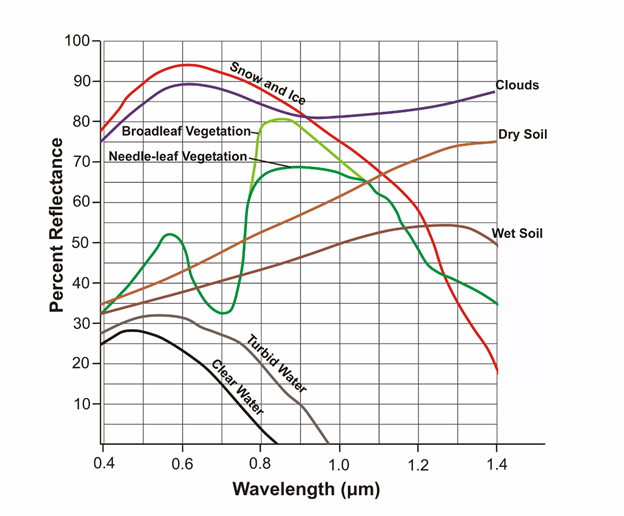
\includegraphics[width=0.8\linewidth]{images/01-spectral-reflectance-characteristics} 

}

\caption{Reflectance characteristics of various features at different wavelengths.}\label{fig:01-spectral-reflectance-characteristics}
\end{figure}

\hypertarget{q1.-for-broadleaf-and-needle-leaf-vegetation-what-is-the-approximate-wavelength-that-is-reflected-most-and-what-section-of-the-ems-does-this-range-belong-to}{%
\paragraph*{Q1. For broadleaf and needle-leaf vegetation, what is the approximate wavelength that is reflected most and what section of the EMS does this range belong to?}\label{q1.-for-broadleaf-and-needle-leaf-vegetation-what-is-the-approximate-wavelength-that-is-reflected-most-and-what-section-of-the-ems-does-this-range-belong-to}}
\addcontentsline{toc}{paragraph}{Q1. For broadleaf and needle-leaf vegetation, what is the approximate wavelength that is reflected most and what section of the EMS does this range belong to?}

\begin{itemize}
\tightlist
\item
  \textbf{0.8-1.0 mm (near infrared)}
\item
  \textbf{0.1-1.0 mm (visible) }
\item
  \textbf{0.7-0.8 mm (near infrared) }
\item
  \textbf{0.55-0.65 mm (visible) }
\end{itemize}

\hypertarget{q2.-truefalse-soil-and-vegetation-reflect-roughly-the-same-proportion-of-blue-light.}{%
\paragraph*{Q2. True/False: Soil and vegetation reflect roughly the same proportion of blue light.}\label{q2.-truefalse-soil-and-vegetation-reflect-roughly-the-same-proportion-of-blue-light.}}
\addcontentsline{toc}{paragraph}{Q2. True/False: Soil and vegetation reflect roughly the same proportion of blue light.}

\hypertarget{q3.-give-a-wavelength-in-microns-mm-at-which-snow-and-ice-dry-soil-and-vegetation-are-indistinguishable-by-their-reflectance.-in-other-words-at-which-wavelength-is-the-proportion-of-radiation-reflected-the-same---10-for-these-features}{%
\paragraph*{Q3. Give a wavelength (in microns; mm) at which snow and ice, dry soil, and vegetation are indistinguishable by their reflectance. In other words, at which wavelength is the proportion of radiation reflected the same (+/- 10\%) for these features?}\label{q3.-give-a-wavelength-in-microns-mm-at-which-snow-and-ice-dry-soil-and-vegetation-are-indistinguishable-by-their-reflectance.-in-other-words-at-which-wavelength-is-the-proportion-of-radiation-reflected-the-same---10-for-these-features}}
\addcontentsline{toc}{paragraph}{Q3. Give a wavelength (in microns; mm) at which snow and ice, dry soil, and vegetation are indistinguishable by their reflectance. In other words, at which wavelength is the proportion of radiation reflected the same (+/- 10\%) for these features?}

\hypertarget{q4.-broadleaf-and-needle-leaf-vegetation-reflect-the-same-amount-at-0.7-mu-m.-what-causes-this-is-there-something-contained-in-the-foliage-of-both-types-of-vegetation-which-causes-identical-spectral-signatures-how-does-this-pattern-in-spectral-reflectance-affect-how-we-see-live-vegetation}{%
\paragraph*{\texorpdfstring{Q4. Broadleaf and needle leaf vegetation reflect the same amount at 0.7 \(\mu\) m. What causes this? Is there something contained in the foliage of both types of vegetation which causes identical spectral signatures? How does this pattern in spectral reflectance affect how we see live vegetation?}{Q4. Broadleaf and needle leaf vegetation reflect the same amount at 0.7 \textbackslash mu m. What causes this? Is there something contained in the foliage of both types of vegetation which causes identical spectral signatures? How does this pattern in spectral reflectance affect how we see live vegetation?}}\label{q4.-broadleaf-and-needle-leaf-vegetation-reflect-the-same-amount-at-0.7-mu-m.-what-causes-this-is-there-something-contained-in-the-foliage-of-both-types-of-vegetation-which-causes-identical-spectral-signatures-how-does-this-pattern-in-spectral-reflectance-affect-how-we-see-live-vegetation}}
\addcontentsline{toc}{paragraph}{Q4. Broadleaf and needle leaf vegetation reflect the same amount at 0.7 \(\mu\) m. What causes this? Is there something contained in the foliage of both types of vegetation which causes identical spectral signatures? How does this pattern in spectral reflectance affect how we see live vegetation?}

\hypertarget{q5.-figure-reffig01-reflectance-characteristics-unknown-features-contains-additional-spectra-belonging-to-unknown-surface-features.-hypothesize-about-what-these-spectra-might-be-and-provude-your-reasoning.-use-the-known-features-broadleaf-vegetation-wet-soil-etc.-and-what-you-have-learned-from-classreadings-to-inform-your-choices.-this-is-a-difficult-task-and-educated-guesses-are-all-that-is-asked-for.-do-a-bit-of-research-put-some-thought-into-it-and-explain-the-reasoning-for-your-guesses.-these-spectra-do-not-represent-the-features-which-are-already-labeled.-you-must-think-of-new-features-which-could-be-observed-with-remote-sensing.}{%
\paragraph*{Q5. Figure \ref{fig:01-reflectance-characteristics-unknown-features} contains additional spectra, belonging to unknown surface features. Hypothesize about what these spectra might be and provude your reasoning. Use the known features (broadleaf vegetation, wet soil, etc.) and what you have learned from class/readings to inform your choices. This is a difficult task, and educated guesses are all that is asked for. Do a bit of research, put some thought into it, and explain the reasoning for your guesses. These spectra do NOT represent the features which are already labeled. You must think of new features which could be observed with remote sensing.}\label{q5.-figure-reffig01-reflectance-characteristics-unknown-features-contains-additional-spectra-belonging-to-unknown-surface-features.-hypothesize-about-what-these-spectra-might-be-and-provude-your-reasoning.-use-the-known-features-broadleaf-vegetation-wet-soil-etc.-and-what-you-have-learned-from-classreadings-to-inform-your-choices.-this-is-a-difficult-task-and-educated-guesses-are-all-that-is-asked-for.-do-a-bit-of-research-put-some-thought-into-it-and-explain-the-reasoning-for-your-guesses.-these-spectra-do-not-represent-the-features-which-are-already-labeled.-you-must-think-of-new-features-which-could-be-observed-with-remote-sensing.}}
\addcontentsline{toc}{paragraph}{Q5. Figure \ref{fig:01-reflectance-characteristics-unknown-features} contains additional spectra, belonging to unknown surface features. Hypothesize about what these spectra might be and provude your reasoning. Use the known features (broadleaf vegetation, wet soil, etc.) and what you have learned from class/readings to inform your choices. This is a difficult task, and educated guesses are all that is asked for. Do a bit of research, put some thought into it, and explain the reasoning for your guesses. These spectra do NOT represent the features which are already labeled. You must think of new features which could be observed with remote sensing.}

\begin{figure}

{\centering 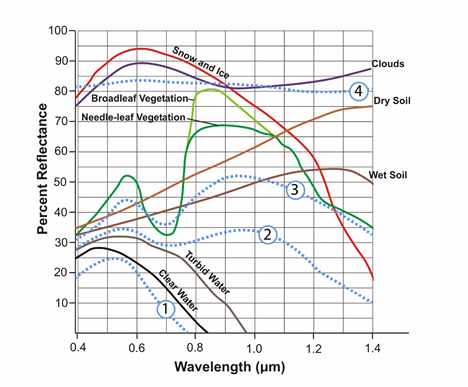
\includegraphics[width=0.8\linewidth]{images/01-reflectance-characteristics-unknown-features} 

}

\caption{Reflectance characteristics of unknown features.}\label{fig:01-reflectance-characteristics-unknown-features}
\end{figure}

\hypertarget{task-2-landsat-5-bands-the-ems-arcgis-pro-software}{%
\section*{Task 2: Landsat 5 Bands, the EMS, \& ArcGIS Pro Software}\label{task-2-landsat-5-bands-the-ems-arcgis-pro-software}}
\addcontentsline{toc}{section}{Task 2: Landsat 5 Bands, the EMS, \& ArcGIS Pro Software}

\begin{longtable}[]{@{}
  >{\raggedright\arraybackslash}p{(\columnwidth - 8\tabcolsep) * \real{0.0701}}
  >{\raggedright\arraybackslash}p{(\columnwidth - 8\tabcolsep) * \real{0.2102}}
  >{\raggedright\arraybackslash}p{(\columnwidth - 8\tabcolsep) * \real{0.1274}}
  >{\raggedright\arraybackslash}p{(\columnwidth - 8\tabcolsep) * \real{0.2102}}
  >{\raggedright\arraybackslash}p{(\columnwidth - 8\tabcolsep) * \real{0.3822}}@{}}
\toprule\noalign{}
\begin{minipage}[b]{\linewidth}\raggedright
\textbf{Bands}
\end{minipage} & \begin{minipage}[b]{\linewidth}\raggedright
\textbf{Wavelength Range (microns)}
\end{minipage} & \begin{minipage}[b]{\linewidth}\raggedright
\textbf{Spectral Region}
\end{minipage} & \begin{minipage}[b]{\linewidth}\raggedright
\textbf{Spatial Resolution (meters)}
\end{minipage} & \begin{minipage}[b]{\linewidth}\raggedright
\textbf{Applications}
\end{minipage} \\
\midrule\noalign{}
\endhead
\bottomrule\noalign{}
\endlastfoot
1 & 0.45-0.52 & Blue & 30 & Coastal water mapping, differentiation of vegetation and soils. \\
2 & 0.52-0.60 & Green & 30 & Assessment of vegetation vigor. \\
3 & 0.63-0.69 & Red & 30 & Chlorophyll absorption for vegetation differentiation. \\
4 & 0.76-0.90 & Near infrared & 30 & Biomass surveys and delineation of water bodies. \\
5 & 1.55-1.75 & Middle infrared & 30 & Vegetation and soil moisture measurements. Differentiation of ice and clouds. \\
6 & 10.40-12.50 & Thermal infrared & 60 & Thermal mapping, soil moisture studies, plant heat stress measurement. \\
7 & 2.08-2.35 & Middle Infrared & 30 & Hydrothermal mapping. \\
8 & 0.52-0.90 & Green, Red, Near infrared & 15 & Panchromatic band. Large area mapping, urban change studies. \\
\end{longtable}

\hypertarget{q6.-each-pixel-of-landsats-thermal-infrared-band-band-6-covers-_____-pixels-of-the-other-bands.-if-it-helps-draw-a-picture-of-the-two-pixel-resolutions.}{%
\paragraph*{Q6. Each pixel of Landsat's thermal infrared band (Band 6) covers \_\_\_\_\_ pixels of the other bands. If it helps, draw a picture of the two pixel resolutions.}\label{q6.-each-pixel-of-landsats-thermal-infrared-band-band-6-covers-_____-pixels-of-the-other-bands.-if-it-helps-draw-a-picture-of-the-two-pixel-resolutions.}}
\addcontentsline{toc}{paragraph}{Q6. Each pixel of Landsat's thermal infrared band (Band 6) covers \_\_\_\_\_ pixels of the other bands. If it helps, draw a picture of the two pixel resolutions.}

\hypertarget{q7.-consider-the-equation-q-h-nu-where-q-is-the-energy-in-quanta-h-is-planks-constant-and-nu-is-the-frequency.-band-6-is-recorded-with-a-coarser-resolution-because-thermal-radiation-has-a-very-_____-wavelength.-therefore-there-is-_____-energy-available-to-sense.}{%
\paragraph*{\texorpdfstring{Q7. Consider the equation \(Q = h * \nu\) where \(Q\) is the energy in quanta, \(h\) is Plank's constant, and \(\nu\) is the frequency. Band 6 is recorded with a coarser resolution because thermal radiation has a very \_\_\_\_\_ wavelength. Therefore, there is \_\_\_\_\_ energy available to sense.}{Q7. Consider the equation Q = h * \textbackslash nu where Q is the energy in quanta, h is Plank's constant, and \textbackslash nu is the frequency. Band 6 is recorded with a coarser resolution because thermal radiation has a very \_\_\_\_\_ wavelength. Therefore, there is \_\_\_\_\_ energy available to sense.}}\label{q7.-consider-the-equation-q-h-nu-where-q-is-the-energy-in-quanta-h-is-planks-constant-and-nu-is-the-frequency.-band-6-is-recorded-with-a-coarser-resolution-because-thermal-radiation-has-a-very-_____-wavelength.-therefore-there-is-_____-energy-available-to-sense.}}
\addcontentsline{toc}{paragraph}{Q7. Consider the equation \(Q = h * \nu\) where \(Q\) is the energy in quanta, \(h\) is Plank's constant, and \(\nu\) is the frequency. Band 6 is recorded with a coarser resolution because thermal radiation has a very \_\_\_\_\_ wavelength. Therefore, there is \_\_\_\_\_ energy available to sense.}

\textbf{Step 1:} To start the lab, Open ArcGIS Pro. You should have window that looks like the screenshot below. The ArcGIS Pro theme used to create this lab is Dark. The default theme is likely Light, but if you are interested in changing themes please follow the instructions at this \href{https://pro.arcgis.com/en/pro-app/latest/get-started/general-options.htm}{link}. To open a new project, choose ``Map'' from the ``New Blank Template'' list.

\begin{center}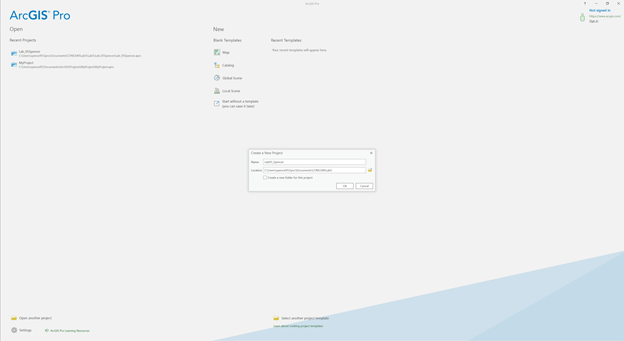
\includegraphics[width=1\linewidth]{images/01-starting-arcgispro-prompt} \end{center}

A prompt will appear requesting you to Name and state the location of your project. It is recommended to name your project ``LabXX\_yourlastname''. Uncheck the ``Create a new folder for this project'' box. As usual, save your project on the (C:) drive in the same folder that your downloaded data is located.

The next window is the generic start of a new project in ArcGIS Pro. In the centre you will see the standard ``Catalog'' frame. At the top is the ribbon, which is where the majority of your analysis options can be found. On the left is the standard ``Contents'' frame, which is similar to that of other Esri products. Tabs can be found on the right-hand side of the window. When using tools or adjusting symbology, be sure to look here for a relevant tab before exploring the ribbon.

You will also notice that the Catolog frame is also ``tabbed''. This means that you can close the frame without closing ArcGIS Pro. It also means that you can have Maps, Catalogs and 3D Scenes all open at the same time. Although this is very cool, be aware that too many tabs are likely to crash ArcGIS Pro. Know your computers processing limits and play within it.

\textbf{Step 2:} Without closing the Catalog window, navigate to the ``Insert'' tab on the ribbon and click on the ``New Map'' icon.

\begin{center}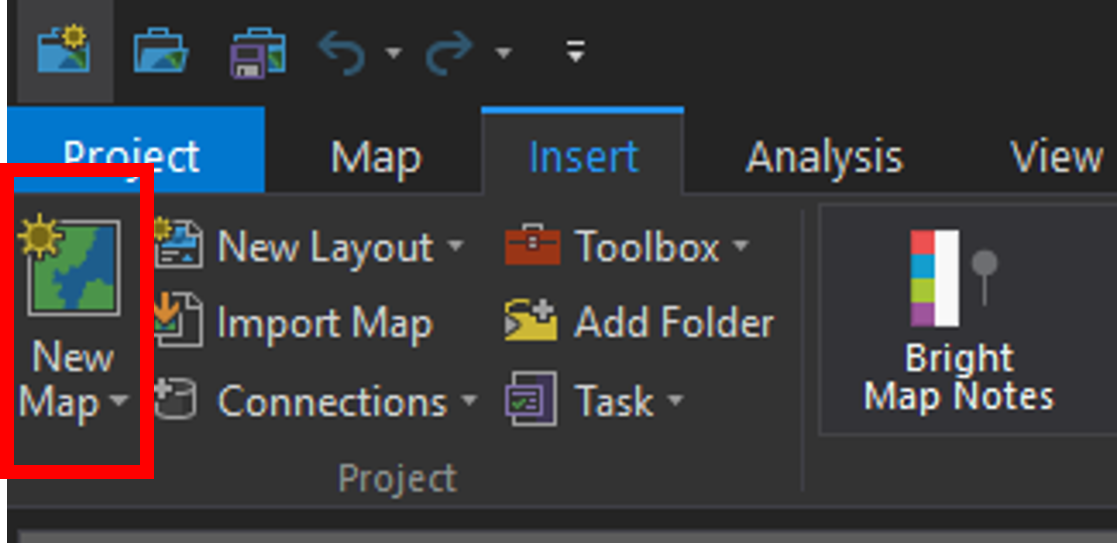
\includegraphics[width=0.5\linewidth]{images/01-new-map} \end{center}

A new topographic map will appear in the centre window. Note that it is separate from the Catalog tab. You can switch back and forth between these as you wish, but recall that there is another Catalog tab on the right-hand side of the screen. When analyzing a map or editing a model, this is the easiest tab to use. For the remainder of the lab, when ``Catalog'' is mentioned it is referring to this side tab.

\textbf{Step 3:} To add data to the map, navigate to the Pre-Lab folder using Catalog* ,if you save your project in the same folder as you data it should appear, if not right click \textbf{Folders} in the Catalog pane and select:

\begin{center}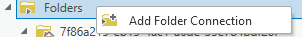
\includegraphics[width=0.5\linewidth]{images/01-add-folder-connection} \end{center}

\textbf{Step 4:} Navigate to where the data is saved and click ok. When you can find the data folder, drag-and-drop the \textbf{L5047026subset\_19990922\_7B.dat} file into the map window. At this point, you should see an RGB satellite image of the city of Vancouver (Figure \ref{fig:01-true-colour-composite-vancouver}) if the mapview does not immediately pan to the image right click \textbf{L5047026subset\_19990922\_7B.dat} in the Contents pane and press Zoom to Layer.

\emph{Note: If the catalog pane does not immediately appear in your ArcGIS Pro document use the ribbons at the top to navigate to \textbf{View -\textgreater{} Catalog Pane}}

\begin{center}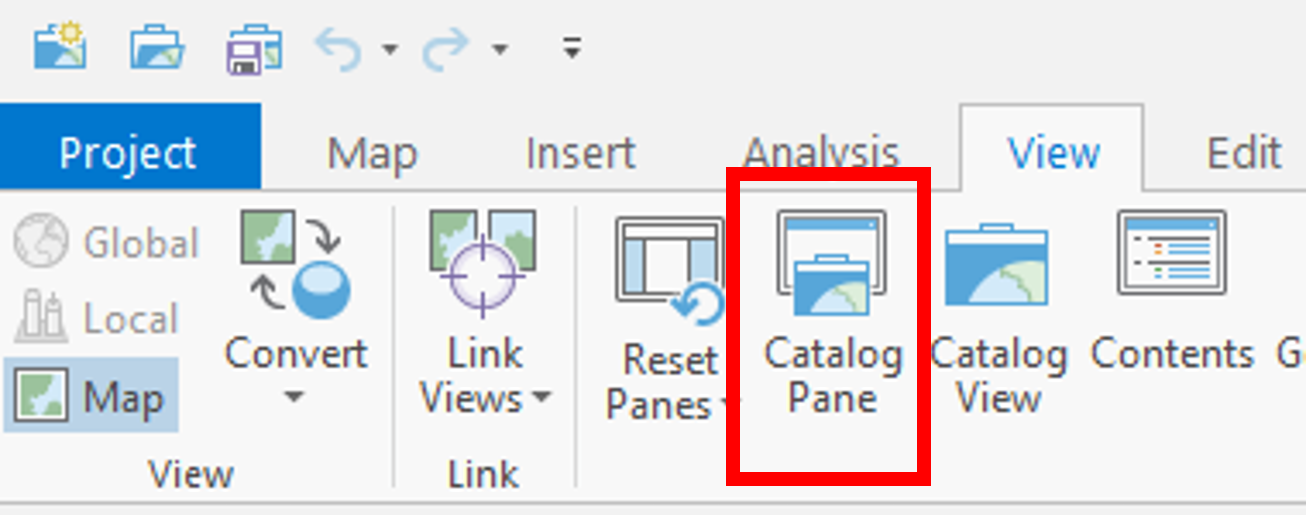
\includegraphics[width=0.5\linewidth]{images/01-catalog-pane} \end{center}

\begin{figure}

{\centering 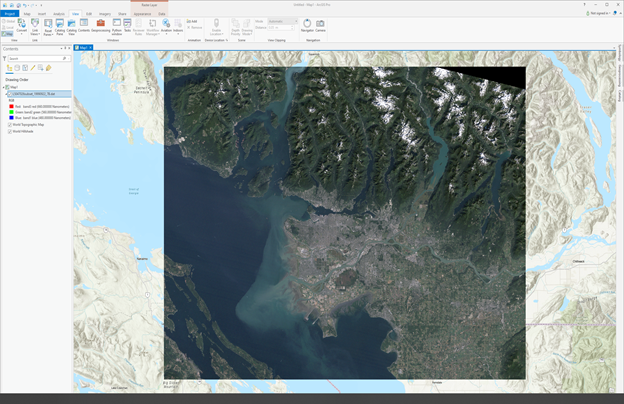
\includegraphics[width=1\linewidth]{images/01-true-colour-composite-vancouver} 

}

\caption{True colour composite of Vancouver.}\label{fig:01-true-colour-composite-vancouver}
\end{figure}

\textbf{Step 5:} It is now time to explore your imagery. Right-click the L5047026subset\_19990922\_7B.dat file in the Contents pane and select ``Properties''. Use the menu on the left-hand side and select the ``Source'' page and the Raster Information drop down.

\begin{center}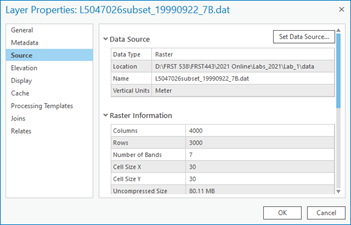
\includegraphics[width=0.5\linewidth]{images/01-raster-information-drop-down} \end{center}

\textbf{Step 6:} After clicking on the \textbf{Raster Information}, the tab should open up, and display important information about the image, such as dimensions (number of pixels in the X or Y directions), data types, projection, and resolution (listed as Projection/Pixel). This information can be useful when examining an image!

\textbf{Step 7:} From the \textbf{Raster Information} you can see that the spatial resolution of this image is approximately 30 m by 30 m, square. That means that each pixel in the image represents an area of approximately 30 x 30 m on the ground, or 900 square meters. Furthermore, it is a Landsat 5 Thematic Mapper image of Vancouver and its surroundings taken at 22 September 1999 - Wow! Even more details are apparent -- its size is 4000 by 3000 pixels, and has seven bands.

\textbf{Step 8:} Scroll down and press on the \textbf{Spatial Reference} to see the projection information.

We will now use ArcGIS Pro to zoom and pan our image.

\textbf{Step 9:} Notice the \textbf{Map} ribbon at the top, navigate to it and hover you mouse of the \textbf{Explore} tool:

\begin{center}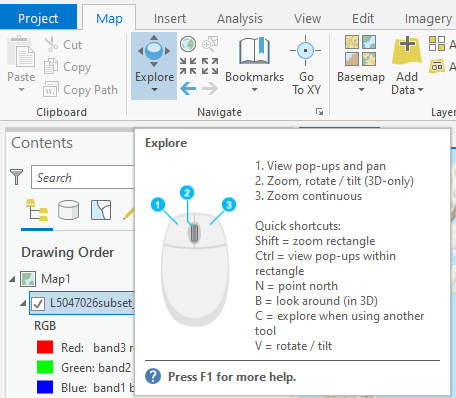
\includegraphics[width=0.5\linewidth]{images/01-explore-tool} \end{center}

Use these controls to zoom in and out of the image and to pan around, try to zoom into the Fraser estuary and navigate upriver. Included in the Navigate pane there are also the fixed zoom tools the previous extent arrows and the small globe which will zoom to the full extent of your data.

Traditionally, single bands of imagery are shown in greyscale, with dark areas shown in black, and light areas shown in white, with anything else shown in shades of grey. Think of each pixel representing a number between 0-255 (byte data type range, the same one of this very imagery!), with areas colored pure black representing the number 0, and areas colored pure white representing the number 255, and everything else is a shade of grey increasing in lightness from 1-254. The figure below displays this concept.

\begin{center}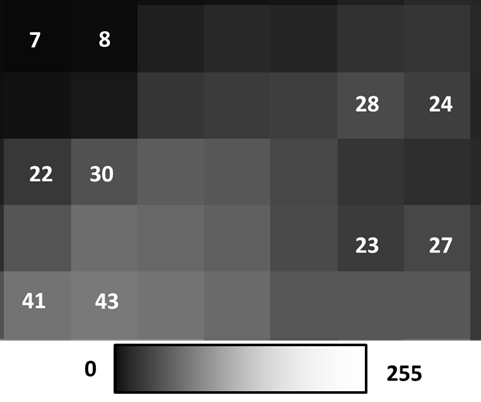
\includegraphics[width=0.5\linewidth]{images/01-grey-scale} \end{center}

\textbf{Step 10:} Right-click on you data in the Contents pane and select ``Symbology''. The symbology pane should appear on the side of you window. Press the drop-down menu and select ``Stretch''.

\begin{center}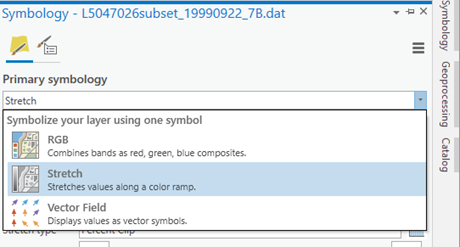
\includegraphics[width=0.5\linewidth]{images/01-symbology-stretch} \end{center}

\textbf{Step 11:} In the next dropdown menu labeled ``Band'' select ``Band 4 NIR'' you should see the same image as below.

\begin{center}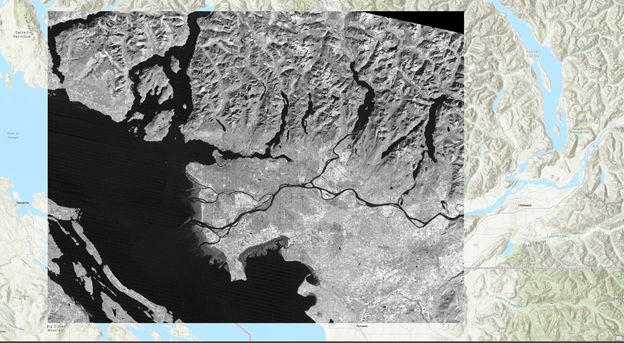
\includegraphics[width=1\linewidth]{images/01-band-4-nir} \end{center}

You have now displayed a single band of greyscale imagery. Pixels that are bright/light/white have high amounts of light being reflected back to the sensor in this section of the EMS. Pixels that are dark/black have high amounts of absorption in this section of the EMS. Pixels are colored by the actual numeric values which indicate how much reflected light the sensor detected (from 0-255). This is a critical component to understand about remote sensing data sets.

When more than 1 spectral band is available for a given image (like the Landsat data provided), colours can be used for visualization. Computer monitors display visible light as combinations of red, green, and blue using the RGB colour model.

\emph{Note: Remember that the colours we see are also a wavelength in the EMS. e.g.~Red -- 660 nm, Green -- 560 nm, Blue -- 480 nm}

In a true colour image, the computer display visualizes objects the way we see them in real life. In other words, in a true colour image, Landsat band 1 (Blue -- 480 nm) is displayed as blue, band 2 (Green -- 560 nm) is displayed as green, and band 3 (Red -- 660 nm) is displayed as red.

Any combination where this is not the case is a \textbf{\emph{false color composite}}, where the colours chosen to visualize the data are not true to life, i.e.~Landsat band 1 (Blue -- 480 nm) is displayed as red, band 2 (Green -- 560 nm) is displayed as blue, and band 3 (Red -- 660 nm) is displayed as green.

Visualizing wavelengths outside of the visible spectrum (Landsat bands 4-7) automatically apply as false colour composites. False colour composites are necessary because many remote sensing devices can measure a broader range of wavelengths than humans can see. As a result, in order to display these data visually for humans, they must be displayed using a part of the spectrum that humans can see (Red, Green, Blue).

\textbf{Step 12:} In the \textbf{Symbology} pane navigate back to ``RGB'' in the first dropdown list. Your image should change back into a \textbf{True Colour} Landsat image where band3 red is visualised as red, band 2 green is visualised as green and band1 blue is visualised as blue.

\begin{center}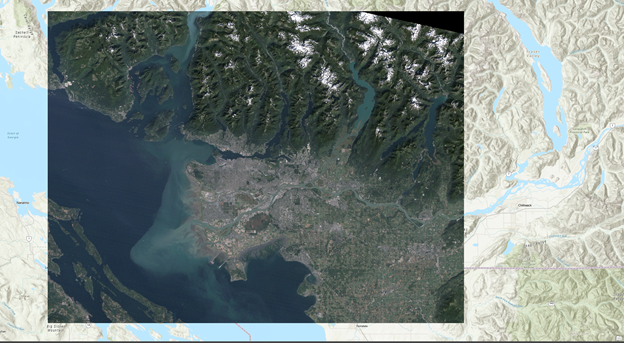
\includegraphics[width=1\linewidth]{images/01-true-colour-landsat-image} \end{center}

By displaying \textbf{false colour composites} it is possible to display many band combinations of the image on our screen. This time you will create a false colour composite by selecting different wavelengths (bands) to be visualized using red, green and blue colours.

\textbf{Step 13:} In the \textbf{Symbology} pane under their respective drop done lists visualize the following band combination.

Band 4 using Red

Band 2 using Green

Band 7 using Blue

You should see the following

\begin{center}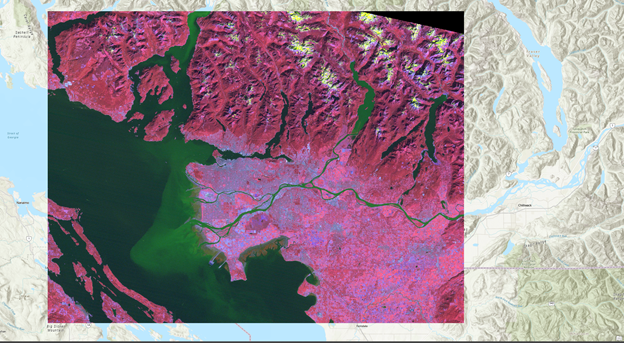
\includegraphics[width=1\linewidth]{images/01-false-colour-composite-pink} \end{center}

You can experiment with different band combinations by visualizing different bands using Red, Green and Blue. A \textbf{standard false colour composite}, for instance, has Band 4 visualized using Red, Band 3 visualized using Green and Band 2 visualized using Blue, as shown below

\begin{center}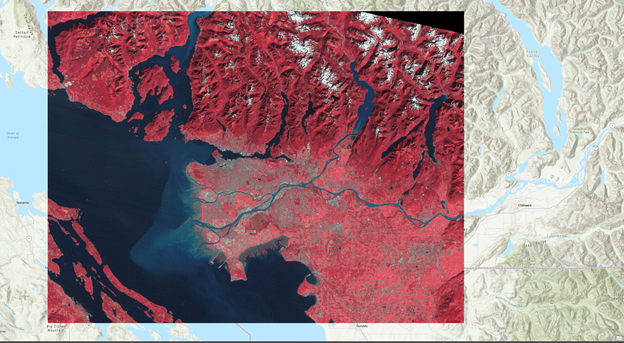
\includegraphics[width=1\linewidth]{images/01-standard-false-colour-composite} \end{center}

Right click the bands in the \textbf{Contents} pane, turn different layers on and off by clicking the check mark off and on in the \textbf{Is Visible} section. Zoom and pan around and investigate different areas of Vancouver that you may know. Feel free to use Google Maps or Google Earth to help you orient yourself.

\hypertarget{q8.-in-a-standard-false-colour-composite-band-4-visualized-used-red-band-3-visualized-using-green-and-band-2-visualized-using-blue-healthy-vegetation-appears-_____.-vegetation-is-more-reflective-in-the-_____-part-of-the-spectrum-than-in-the-green-part-of-the-spectrum-so-_____-appears-the-brightest.}{%
\paragraph*{\texorpdfstring{Q8. In a \textbf{\emph{standard false colour}} composite (Band 4 visualized used red, Band 3 visualized using green, and Band 2 visualized using blue), healthy vegetation appears \_\_\_\_\_. Vegetation is more reflective in the \_\_\_\_\_ part of the spectrum than in the green part of the spectrum so \_\_\_\_\_ appears the brightest.}{Q8. In a standard false colour composite (Band 4 visualized used red, Band 3 visualized using green, and Band 2 visualized using blue), healthy vegetation appears \_\_\_\_\_. Vegetation is more reflective in the \_\_\_\_\_ part of the spectrum than in the green part of the spectrum so \_\_\_\_\_ appears the brightest.}}\label{q8.-in-a-standard-false-colour-composite-band-4-visualized-used-red-band-3-visualized-using-green-and-band-2-visualized-using-blue-healthy-vegetation-appears-_____.-vegetation-is-more-reflective-in-the-_____-part-of-the-spectrum-than-in-the-green-part-of-the-spectrum-so-_____-appears-the-brightest.}}
\addcontentsline{toc}{paragraph}{Q8. In a \textbf{\emph{standard false colour}} composite (Band 4 visualized used red, Band 3 visualized using green, and Band 2 visualized using blue), healthy vegetation appears \_\_\_\_\_. Vegetation is more reflective in the \_\_\_\_\_ part of the spectrum than in the green part of the spectrum so \_\_\_\_\_ appears the brightest.}

\hypertarget{q9.-experiment-with-many-different-false-colour-composites.-which-3-bands-would-you-combine-if-you-wanted-to-analyze-vegetation-do-some-light-research-on-spectral-properties-and-the-applications-of-different-landsat-bands-and-write-a-sentence-or-two-justifying-each-of-your-choices.-then-append-a-screenshot-of-your-chosen-composite-to-your-response.}{%
\paragraph*{\texorpdfstring{Q9. Experiment with many different false colour composites. Which 3 bands would you combine if you wanted to analyze \textbf{vegetation}? Do some light research on spectral properties and the applications of different Landsat bands and write a sentence or two justifying each of your choices. Then, append a screenshot of your chosen composite to your response.}{Q9. Experiment with many different false colour composites. Which 3 bands would you combine if you wanted to analyze vegetation? Do some light research on spectral properties and the applications of different Landsat bands and write a sentence or two justifying each of your choices. Then, append a screenshot of your chosen composite to your response.}}\label{q9.-experiment-with-many-different-false-colour-composites.-which-3-bands-would-you-combine-if-you-wanted-to-analyze-vegetation-do-some-light-research-on-spectral-properties-and-the-applications-of-different-landsat-bands-and-write-a-sentence-or-two-justifying-each-of-your-choices.-then-append-a-screenshot-of-your-chosen-composite-to-your-response.}}
\addcontentsline{toc}{paragraph}{Q9. Experiment with many different false colour composites. Which 3 bands would you combine if you wanted to analyze \textbf{vegetation}? Do some light research on spectral properties and the applications of different Landsat bands and write a sentence or two justifying each of your choices. Then, append a screenshot of your chosen composite to your response.}

\hypertarget{q10.-experiment-with-many-different-false-colour-composites.-which-3-bands-would-you-combine-if-you-wanted-to-analyze-water-quality-do-some-light-research-on-spectral-properties-and-the-applications-of-different-landsat-bands-and-write-a-sentence-or-two-justifying-each-of-your-choices.-then-append-a-screenshot-of-your-chosen-composite-to-your-response.}{%
\paragraph*{\texorpdfstring{Q10. Experiment with many different false colour composites. Which 3 bands would you combine if you wanted to analyze \textbf{water quality}? Do some light research on spectral properties and the applications of different Landsat bands and write a sentence or two justifying each of your choices. Then, append a screenshot of your chosen composite to your response.}{Q10. Experiment with many different false colour composites. Which 3 bands would you combine if you wanted to analyze water quality? Do some light research on spectral properties and the applications of different Landsat bands and write a sentence or two justifying each of your choices. Then, append a screenshot of your chosen composite to your response.}}\label{q10.-experiment-with-many-different-false-colour-composites.-which-3-bands-would-you-combine-if-you-wanted-to-analyze-water-quality-do-some-light-research-on-spectral-properties-and-the-applications-of-different-landsat-bands-and-write-a-sentence-or-two-justifying-each-of-your-choices.-then-append-a-screenshot-of-your-chosen-composite-to-your-response.}}
\addcontentsline{toc}{paragraph}{Q10. Experiment with many different false colour composites. Which 3 bands would you combine if you wanted to analyze \textbf{water quality}? Do some light research on spectral properties and the applications of different Landsat bands and write a sentence or two justifying each of your choices. Then, append a screenshot of your chosen composite to your response.}

\hypertarget{q11.-experiment-with-many-different-false-colour-composites.-which-3-bands-would-you-combine-if-you-wanted-to-analyze-agriculture-do-some-light-research-on-spectral-properties-and-the-applications-of-different-landsat-bands-and-write-a-sentence-or-two-justifying-each-of-your-choices.-then-append-a-screenshot-of-your-chosen-composite-to-your-response.}{%
\paragraph*{\texorpdfstring{Q11. Experiment with many different false colour composites. Which 3 bands would you combine if you wanted to analyze \textbf{agriculture}? Do some light research on spectral properties and the applications of different Landsat bands and write a sentence or two justifying each of your choices. Then, append a screenshot of your chosen composite to your response.}{Q11. Experiment with many different false colour composites. Which 3 bands would you combine if you wanted to analyze agriculture? Do some light research on spectral properties and the applications of different Landsat bands and write a sentence or two justifying each of your choices. Then, append a screenshot of your chosen composite to your response.}}\label{q11.-experiment-with-many-different-false-colour-composites.-which-3-bands-would-you-combine-if-you-wanted-to-analyze-agriculture-do-some-light-research-on-spectral-properties-and-the-applications-of-different-landsat-bands-and-write-a-sentence-or-two-justifying-each-of-your-choices.-then-append-a-screenshot-of-your-chosen-composite-to-your-response.}}
\addcontentsline{toc}{paragraph}{Q11. Experiment with many different false colour composites. Which 3 bands would you combine if you wanted to analyze \textbf{agriculture}? Do some light research on spectral properties and the applications of different Landsat bands and write a sentence or two justifying each of your choices. Then, append a screenshot of your chosen composite to your response.}

\hypertarget{q12.-experiment-with-many-different-false-colour-composites.-which-3-bands-would-you-combine-if-you-wanted-to-analyze-urban-areas-do-some-light-research-on-spectral-properties-and-the-applications-of-different-landsat-bands-and-write-a-sentence-or-two-justifying-each-of-your-choices.-then-append-a-screenshot-of-your-chosen-composite-to-your-response.}{%
\paragraph*{\texorpdfstring{Q12. Experiment with many different false colour composites. Which 3 bands would you combine if you wanted to analyze \textbf{urban areas}? Do some light research on spectral properties and the applications of different Landsat bands and write a sentence or two justifying each of your choices. Then, append a screenshot of your chosen composite to your response.}{Q12. Experiment with many different false colour composites. Which 3 bands would you combine if you wanted to analyze urban areas? Do some light research on spectral properties and the applications of different Landsat bands and write a sentence or two justifying each of your choices. Then, append a screenshot of your chosen composite to your response.}}\label{q12.-experiment-with-many-different-false-colour-composites.-which-3-bands-would-you-combine-if-you-wanted-to-analyze-urban-areas-do-some-light-research-on-spectral-properties-and-the-applications-of-different-landsat-bands-and-write-a-sentence-or-two-justifying-each-of-your-choices.-then-append-a-screenshot-of-your-chosen-composite-to-your-response.}}
\addcontentsline{toc}{paragraph}{Q12. Experiment with many different false colour composites. Which 3 bands would you combine if you wanted to analyze \textbf{urban areas}? Do some light research on spectral properties and the applications of different Landsat bands and write a sentence or two justifying each of your choices. Then, append a screenshot of your chosen composite to your response.}

Now it is time to examine your data set more thoroughly. At the beginning of this lab we examined the spectral signatures of different materials. We will now do the same thing for the different sections of our Vancouver Landsat image.

\textbf{Step 14:} Right-click on the \textbf{L5047026subset\_19990922\_7B.dat} file in the Contents pane and select \textbf{Create Chart -\textgreater{} Spectral Profile}. The Chart Properties pane should appear on the right side of your screen and the spectral chart on the bottom.

\begin{center}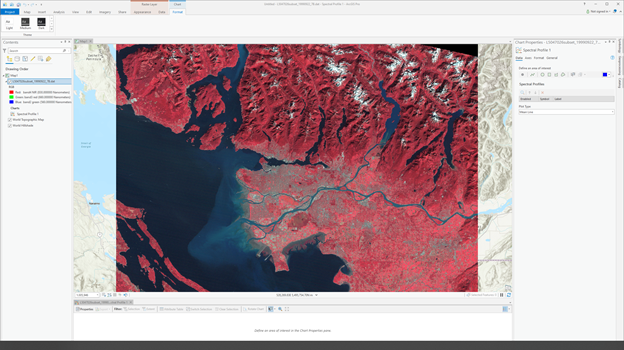
\includegraphics[width=1\linewidth]{images/01-create-spectral-profile} \end{center}

In the Chart properties pane under ``Define an Area of Interest'' select ``point'' and then click a pixel on your map. Change the colour and select a variety of different points representing different land cover types (Urban, forest, water, crops, snow).

\begin{center}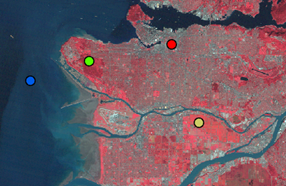
\includegraphics[width=0.5\linewidth]{images/01-area-of-interest-points} \end{center}

You might have to resize the spectral chart at the bottom of your screen in order to see the different profiles. Your chart should look something like this:

\begin{center}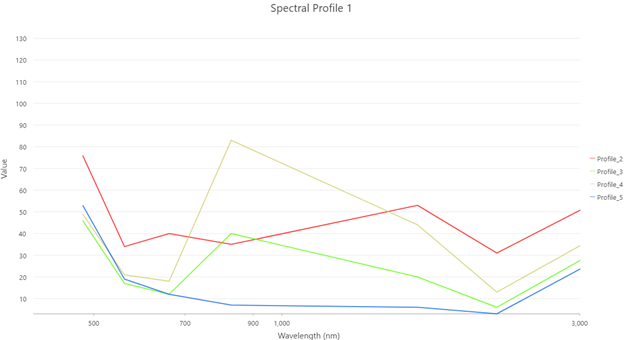
\includegraphics[width=1\linewidth]{images/01-profile-chart} \end{center}

\hypertarget{q13.-examine-your-new-spectral-profile-chart-compare-the-different-profiles-you-created-to-the-spectral-profiles-in-figures-1-and-2.-what-is-the-difference-between-them-why-might-your-spectral-curves-look-different-than-the-ones-above-take-a-screenshot-of-your-spectral-signature-chart-and-append-it-to-your-answer.}{%
\paragraph*{Q13. Examine your new spectral profile chart, compare the different profiles you created to the spectral profiles in figures 1 and 2. What is the difference between them? Why might your spectral curves look different than the ones above? Take a screenshot of your spectral signature chart and append it to your answer.}\label{q13.-examine-your-new-spectral-profile-chart-compare-the-different-profiles-you-created-to-the-spectral-profiles-in-figures-1-and-2.-what-is-the-difference-between-them-why-might-your-spectral-curves-look-different-than-the-ones-above-take-a-screenshot-of-your-spectral-signature-chart-and-append-it-to-your-answer.}}
\addcontentsline{toc}{paragraph}{Q13. Examine your new spectral profile chart, compare the different profiles you created to the spectral profiles in figures 1 and 2. What is the difference between them? Why might your spectral curves look different than the ones above? Take a screenshot of your spectral signature chart and append it to your answer.}

\begin{center}\rule{0.5\linewidth}{0.5pt}\end{center}

\hypertarget{summary}{%
\section*{Summary}\label{summary}}
\addcontentsline{toc}{section}{Summary}

In this lab, we introduced concepts of using specific ranges of the electromagnetic spectrum to understand spectral reflectance and spectral signatures. Spectral signatures are determined by the spectral properties of different materials. They can be used to gather more information about a material than what we can see with visible light! We used ArcGIS Pro to analyze different types of remote sensing data and visualized various combinations of bands using greyscale, true colour composites, and false colour composites. This lab is just the beginning of our remote sensing journey but opens our eyes to the power of remote sensing and its ability to unveil information about the world around us!

Return to the \protect\hyperlink{lab1-deliverables}{\textbf{Deliverables}} section to check off everything you need to submit for credit in the course management system.

\hypertarget{network-analysis}{%
\chapter{Salmon Stream Network Analysis}\label{network-analysis}}

Written by
Paul Pickell

\hypertarget{lab-overview-1}{%
\section*{Lab Overview}\label{lab-overview-1}}
\addcontentsline{toc}{section}{Lab Overview}

An important application of GIS for watershed management is characterizing the physical components of streams, rivers, and water bodies. In this lab, you will learn how to use the Hydrology, Network Analyst, and Linear Referencing toolsets in ArcGIS Pro to extract hydrologic information from a digital elevation model (DEM) in order to model a network of streams.

In British Columbia, salmon are an important species for economic, cultural, and ecological reasons. Thus, there is extensive research and management efforts to better understand and sustainably manage salmon populations. There are five Pacific salmon species, Chinook, Coho, Chum, Pink, and Sockeye salmon. Salmon are diadromous species, spending their lifecycle in both freshwater and the ocean. We are particularly interested in habitat for salmon spawning. Salmon return to freshwater habitats to spawn and there are various requirements for salmon spawning that differ by species:

\begin{itemize}
\item
  Stream order
\item
  Proximity to a lake
\item
  Upwelling/downwelling
\item
  Water quality
\item
  Water depth
\item
  Water velocity
\item
  Substrate material
\item
  Slope gradient
\item
  Land cover
\end{itemize}

For this lab, you will identify the preferred habitat for salmon spawning based on proxy measures and how it corresponds to our stream network that we have derived from the DEM. This lab will walk you through how to measure stream order and slope. For your final report, you will also be expected to analyze an additional habitat requirement for salmon spawning. (Note: if you use some information that is not on the aforementioned list, please describe how it is a habitat requirement for salmon spawning in your report.)

In this lab, we will focus on Vancouver Island for a few reasons. First, islands make it possible to calculate flow accumulation exactly, which is important for creating a (nearly) topologically correct stream network. Second, Vancouver Island is large, which will enable us to look at natural sources of topological errors. Third, many species of Pacific salmon return to highly developed Vancouver Island to spawn and often come into conflict with human development.

\begin{center}\rule{0.5\linewidth}{0.5pt}\end{center}

\hypertarget{learning-objectives-1}{%
\section*{Learning Objectives}\label{learning-objectives-1}}
\addcontentsline{toc}{section}{Learning Objectives}

\begin{itemize}
\item
  Derive hydrology layers from a DEM
\item
  Model dams on streams as barriers by applying network topology
\item
  Evaluate a capability model of salmon habitat along stream segments using linear referencing
\item
  Trace a stream network and calculate reachable upstream salmon habitat
\end{itemize}

\begin{center}\rule{0.5\linewidth}{0.5pt}\end{center}

\hypertarget{lab2-deliverables}{%
\section*{Deliverables}\label{lab2-deliverables}}
\addcontentsline{toc}{section}{Deliverables}

The lab deliverables to be submitted on canvas include:

Lab report with the following specifications:

Map showing the reach of your streams from the ocean with dams as barriers

Map showing the salmon conservation unit that you have selected to focus on

4 pages maximum PDF including findings and anwers to the questions at the end of the lab

Report should satisfy the following requirements:

\begin{itemize}
\tightlist
\item
  1'' margins
\item
  12 point font
\item
  single spaced
\item
  maximum of four pages
\item
  use headings as needed
\item
  omit your name, student number, date
\end{itemize}

\begin{center}\rule{0.5\linewidth}{0.5pt}\end{center}

\hypertarget{data-1}{%
\section*{Data}\label{data-1}}
\addcontentsline{toc}{section}{Data}

\textbf{vancouver\_island\_dem}

To save time for this lab, the DEM has already been assembled and pre-processed for you. This was the general process applied to create the DEM in case you want to reproduce it or apply the same method for another project:

\begin{enumerate}
\def\labelenumi{\arabic{enumi}.}
\tightlist
\item
  Download all the tiles for Vancouver Island from the B.C. Government \href{https://www2.gov.bc.ca/gov/content/data/geographic-data-services/topographic-data/elevation}{here}
\item
  Mosaic the rasters together using the ``Mosaic to new raster'' tool
\item
  Buffer a polygon shapefile of Vancouver Island by 25 m
\item
  Convert the result of step 3 to a raster with cell size 25 m and project to NAD 1983 BC Environment Albers. This is a mask that extends just beyond the shore of Vancouver Island to account for mapping errors.
\item
  Extract the DEM from step 2 by the mask in step 4 to produce a DEM for only Vancouver Island that excludes all other nearby islands:
\end{enumerate}

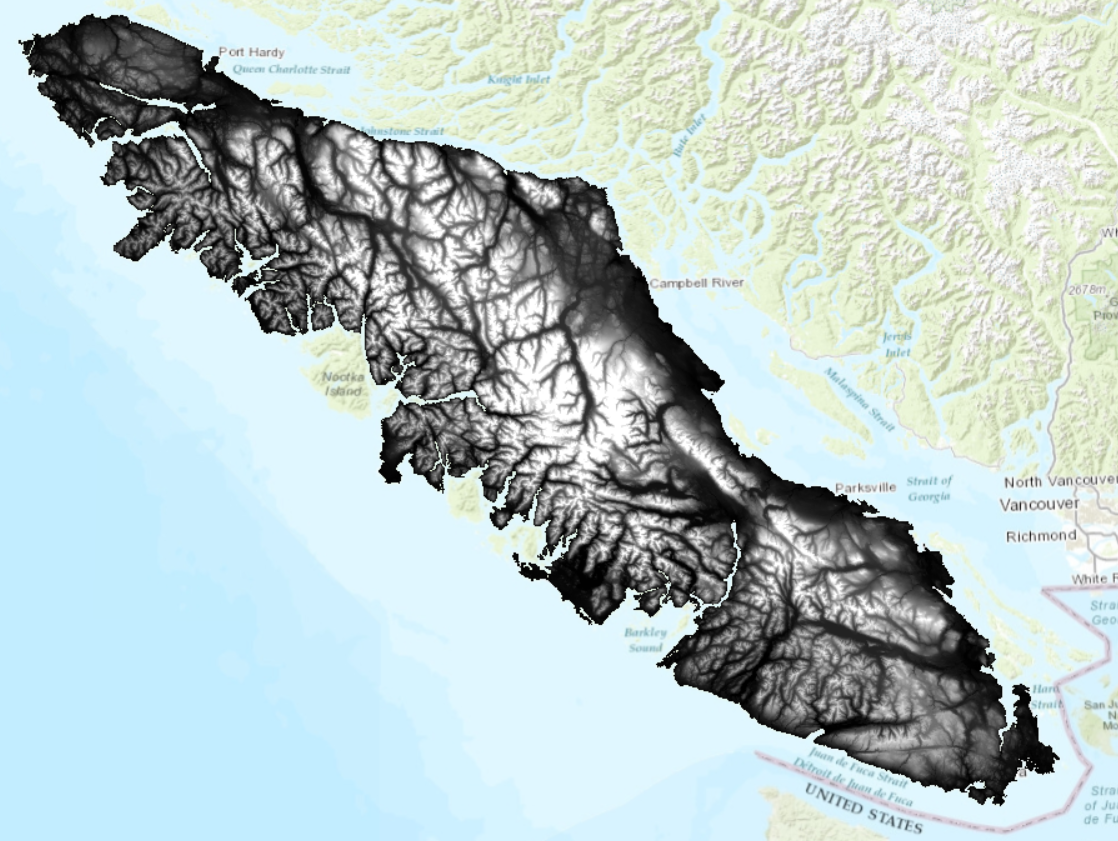
\includegraphics[width=1\linewidth]{images/02-vancouver-island-dem}

\textbf{vancouver\_island\_dem}
The DEM above was filtered several times for sinks. Generally, you can use the ``Fill'' tool to achieve this. However, Vancouver Island has many naturally-occurring geomorphic features that can cause real sinks (as opposed to random errors). In order to create a depressionless DEM, the DEM was iteratively put through the following process:

\begin{enumerate}
\def\labelenumi{\arabic{enumi}.}
\tightlist
\item
  Calculate flow direction
\item
  Calculate sinks
\item
  Calculate watersheds using the flow direction raster and the sinks raster as pour points
\item
  Calculate minimum elevation of the sinks using the ``Zonal statistics'' tool
\item
  Calculate maximum elevation of the watershed for the sink using the ``Zonal fill'' tool
\item
  Subtract result of step 4 from result of step 5 for the sinks mapped in step 2. This is the depth of each sink.
\item
  Add the sink depth to the DEM to fill the sink
\item
  Repeat steps 1-7 several times until you remove all sinks or achieve a stopping criterion
\end{enumerate}

The original DEM contained \textgreater3,000 sinks. After iterating the above 12 times, there were fewer than 300 sinks. You can subtract the DEM from the filled DEM to observe where fill was added. Notice any patterns for where sinks are located on the island?

\textbf{dams}

The dams were acquired from the BC Government \href{https://catalogue.data.gov.bc.ca/dataset/bc-dams}{here}. These data were clipped to Vancouver Island and represent dam structures as polyline features.

\textbf{Salmon conservation units (CU)}

Conservation units for Chinook, Chum, and Coho were acquired from Oceans and Fisheries Canada \href{https://open.canada.ca/data/en/dataset/1ac00a39-4770-443d-8a6b-9656c06df6a3\#wb-auto-6}{here}. These polygon areas were mapped considering ecology, life history, and molecular genetics (\href{https://onlinelibrary.wiley.com/doi/abs/10.1111/j.1095-8649.2001.tb01376.x}{Waples et al 2001}).

\begin{center}\rule{0.5\linewidth}{0.5pt}\end{center}

\hypertarget{task-1-create-stream-segments}{%
\section*{Task 1: Create stream segments}\label{task-1-create-stream-segments}}
\addcontentsline{toc}{section}{Task 1: Create stream segments}

\textbf{Step 1}: Before starting the lab, you will need to download all of the data from the \texttt{salmon} database on the UBC PostgreSQL server. Currently, ArcGIS Pro cannot read Post GIS raster datasets so we will first open the Vancouver Island DEM in QGIS and Export it as a GeoTiff, which can be opened in ArcGIS Pro.

Open QGIS and connect to the \texttt{salmon} PostgreSQL server. Expand the \texttt{salmon} database in the Browser pane and right-click on ``vancouver\_island\_dem'' \textgreater{} Add Layer to Project.

Right click on the DEM layer in the Layers pane \textgreater{} Export \textgreater{} Save as. Save the file as a GeoTiff in your Lab 2 project folder. Leave the default settings. Close QGIS.

\textbf{Step 2:} In ArcGIS Pro, add the Vancouver Island DEM to your map project. Clip the DEM to the''vancouver\_island\_boundary'' using the clip raster tool, toggle on ``use input features for clipping geometry''.

You should save all of your outputs from the tools in this lab directly into your ArcGIS Pro project geodatabase. The reasoning for this is because we will only be working in ArcGIS Pro for this lab and also because the ArcGIS Pro topology tools only work with data inside an ArcGIS Pro geodatabase.

Calculate the flow direction of the filled DEM, using the ``Flow Direction'' tool. The flow direction tool determines which raster cells flow into other cells based on the elevation difference the immediate neighborhood. Keep the defaults of the tool. Ensure that ``Force all edge cells to flow outward'' is toggled on and leave all other parameters with the default value. The cell values in the output raster represent the steepest down slope direction of each pixel.

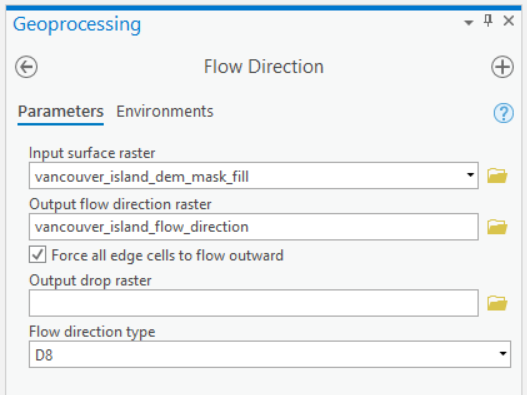
\includegraphics[width=0.5\linewidth]{images/02-flow-direction}

\textbf{Step 3:} Use the output from the ``Flow Direction'' tool as an input into the ``Flow Accumulation'' tool. Again, use the defaults within the tool, but select integer as the output data type because the output of this tool is a count. This tool will create a raster that represents the number of pixels that will accumulate into any given pixel. You may need to zoom into the output to be able to see these streams. Play around with the symbology to visualize the stream network. (Hint: try using classify and various methods within symbology).

\textbf{Step 4:} To define streams, you need to set a threshold for the flow accumulation. Open ``Con''(Image Analyst Tools). This tool allows you to set a true/false condition and assign values to a new raster based on whether the condition is met. Set the expression so that a pixel that has a count equal to or more than 1000 will be assigned a value of 1. For ``Input true raster or constant value'', use value 1. For ``Input false raster or constant value'', use value 0.

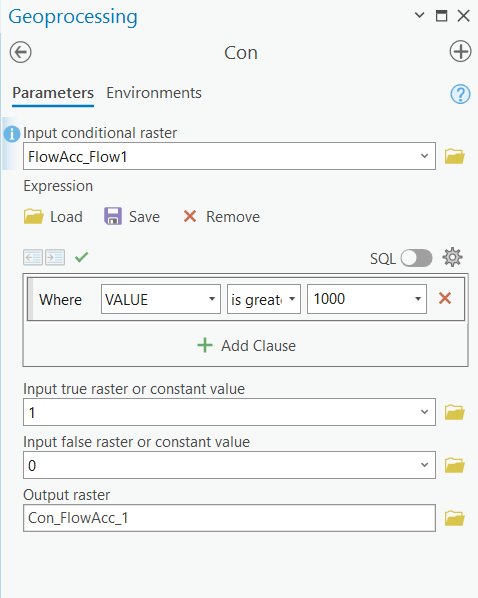
\includegraphics[width=0.5\linewidth]{images/02-con}

\textbf{Step 5:} Next, you will create a grid of stream links, which assigns unique values to each stream segment, so that the user can see how the streams are connected. Open the ``Stream Link'' tool and use the output from the ``Con'' tool and the flow direction raster here.

\textbf{Step 6:} You will also use the ``Stream Order'' tool using the same inputs as in step 4 and the default parameters. The ``Stream Order'' tool assigns a numeric order to segments of the raster, essentially classifying branches of the stream network. The lowest order streams do not have any other streams that flow into it, while higher order streams can have multiple levels of tributaries that flow into it. This tool will take some time to run on the whole island. Take a moment to stretch and hydrate!

\textbf{Step 7:} You will also convert your raster into polylines using the stream links raster and flow direction raster as inputs for the ``Stream to Feature'' tool. Toggle off ``Simplify polylines''.

Below is a useful flowchart of the process of creating a stream network from a DEM (\href{https://pro.arcgis.com/en/pro-app/tool-reference/spatial-analyst/deriving-runoff-characteristics.htm}{ArcGIS Pro}).

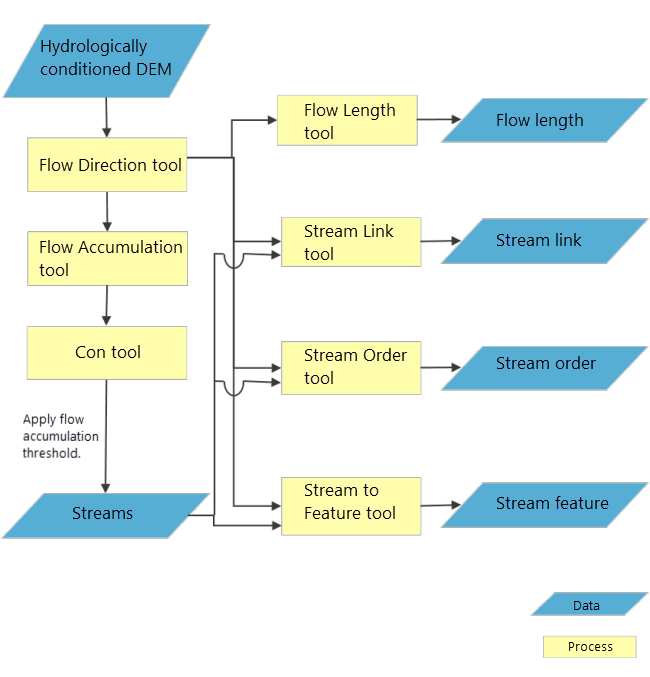
\includegraphics[width=0.75\linewidth]{images/02-flow-chart}

\begin{center}\rule{0.5\linewidth}{0.5pt}\end{center}

\hypertarget{task-2-create-routes-and-apply-topology}{%
\section*{Task 2: Create routes and apply topology}\label{task-2-create-routes-and-apply-topology}}
\addcontentsline{toc}{section}{Task 2: Create routes and apply topology}

At this point, you have only created polyline features representing streams. Next we will convert those segments to routes and apply topology for our streams, as well as incorporate dams into the network.

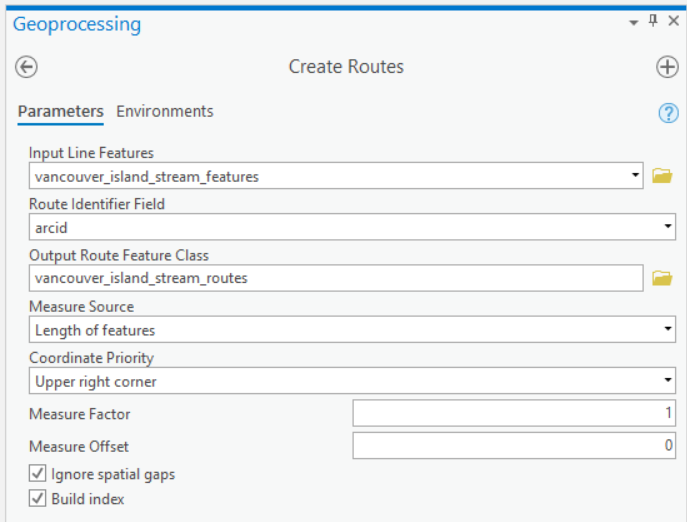
\includegraphics[width=0.75\linewidth]{images/02-create-routes}

\textbf{Step 1:} Create a blank feature dataset and name it ``stream\_routes\_dams''. To do this, right-click the geodatabase in the Catalog pane and select New Feature Dataset. For the projection, use NAD 1983 BC Environment Albers (EPSG: 3005).

\textbf{Step 2:} Convert your stream features into routes using the ``Create routes'' tool. Set the Route ID field to ``arcid''. The coordinate Priority parameter can be set to any corner. When you go to save your output, navigate into your feature dataset (it ``feels'' like entering another folder from the Catalog view), and save the output as ``vancouver\_island\_stream\_routes''.

\textbf{Step 3:} Right-click on the feature dataset, select ``Import'', and then navigate to the \textbf{dams} layer on the UBC PostgreSQL server and import this layer into your feeature dataset.

The dams are modelled as polylines. We need to identify where these dams intersect the stream routes. We want to return a single point for that location so that we can properly model the dams in our network, which act as barriers to salmon as they travel through the stream network. We will use topology to achieve this.

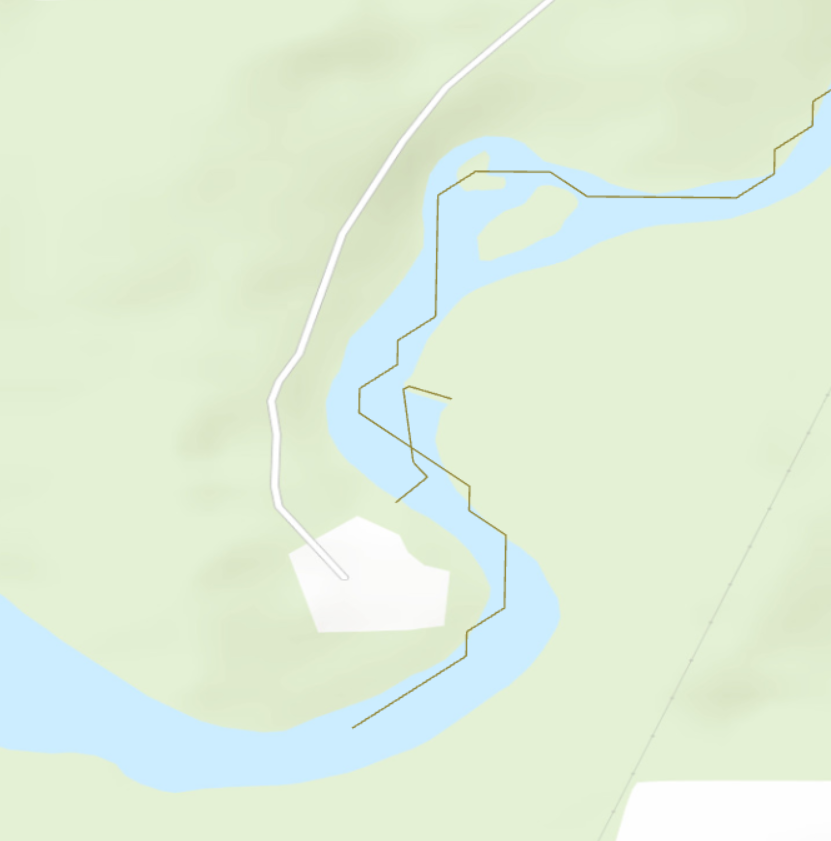
\includegraphics[width=1\linewidth]{images/02-example-dam}

\textbf{Step 4:} Right-click the feature dataset and select ``New'' and ``Topology''. This will open the Create Topology Wizard dialogue box.

\textbf{Step 5:} On the first page of the wizard, toggle on the dams and stream routes feature classes.

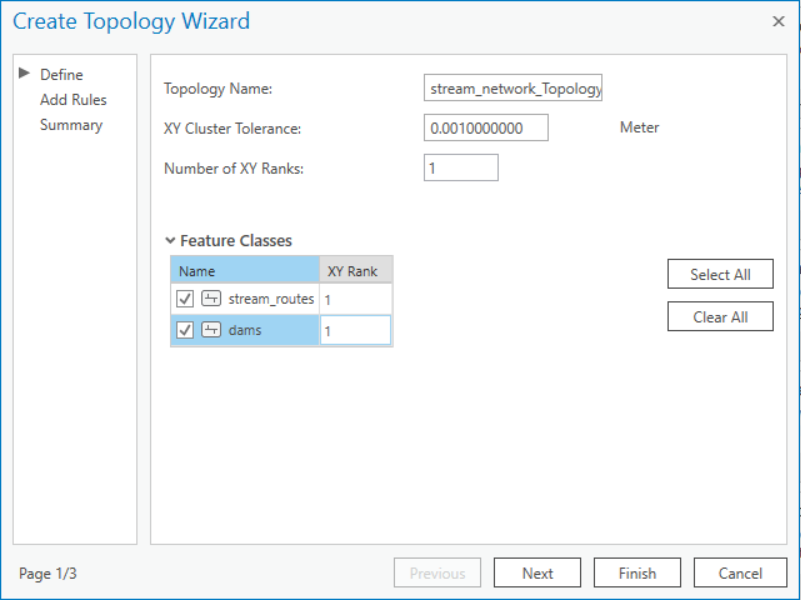
\includegraphics[width=1\linewidth]{images/02-create-topology-1}

\textbf{Step 6:} On the second page of the wizard, add a new rule so that the stream polylines must not intersect with the dam polylines.

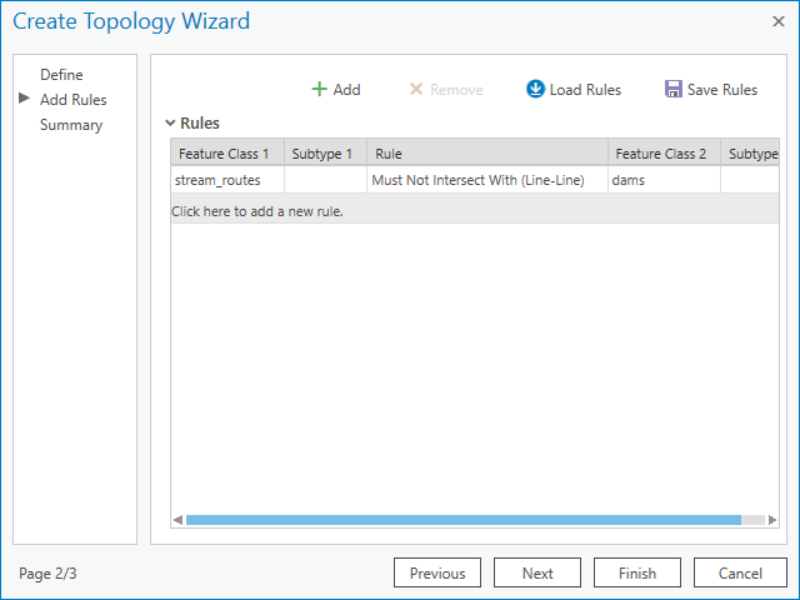
\includegraphics[width=1\linewidth]{images/02-create-topology-2}

Once done, click ``Finish''. Refresh the feature dataset in the Catalog pane to see the new Topology.

\textbf{Step 7:} Validate the topology by right-clicking the topology in the feature dataset and clicking ``Validate''.

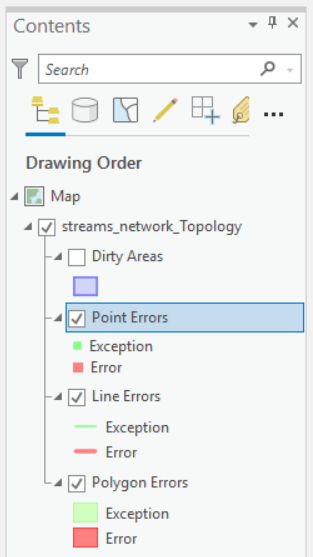
\includegraphics[width=0.25\linewidth]{images/02-topology-errors}

\textbf{Step 8:} You can click and drag the topology into the map to view any errors. We expect there to be errors because we know that the dams should intersect with our stream routes. You should see red squares all over the island. In the Contents Pane, right-click the ``Point Errors'' layer, select ``Data'', and select ``Export Features''. Save the points to your feature dataset as ``stream\_dam\_junctions''.

At this point, take a moment to appreciate where we are in this problem. We have modelled streams as routes and we now know where dams intersect with those routes. Salmon are diadromous species, they swim from the saltwater ocean up the freshwater streams to spawn. Therefore, we need one more piece of information in order to model how salmon swim upstream. We need to know where the streams meet the ocean.

\textbf{Step 9:} Take the Vancouver Island boundary polygon provided and perform a negative buffer, called a nibble. Use -25 meters for the buffer distance. We are doing a negative buffer because we want to ensure that this edge intersects with the streams that terminate at the ocean. Remember that the streams were generated by an imperfect and imprecise DEM, therefore this process will ensure that every stream that reaches the ocean will intersect this boundary.

\textbf{Step 10:} Convert the nibbled Vancouver Island boundary to a polyline using the ``Polygon to line'' tool. Be sure to toggle off ``Identify and store polygon neighboring information''. \textbf{Save the result to your feature dataset with the stream links and dams.}

Next, we will use the same topology process to identify where the island boundary intersects the stream routes, representing where salmon enter the stream network from the ocean.

\textbf{Step 11:} Right-click the network topology in the Catalog and select ``Properties''. This will open the topology wizard dialogue again. On the left, select ``Feature Class'' and toggle on the nibbled Vancouver island boundary that you created in step 10 and the stream routes. Toggle everything else off. On the left, select ``Rules''. Highlight the previous rule and click the ``Remove'' button at the top. Then, add a rule so that the stream routes must not intersect with the nibbled island boundary. Refer to steps 5 and 6 above if you need clarification.

\textbf{Step 12:} Again, validate the topology, add the topology to the map view, and export the Point Errors to a point feature class in your feature dataset. Name it ``stream\_ocean\_junctions''. Refer to steps 7 and 8 if you need clarification.

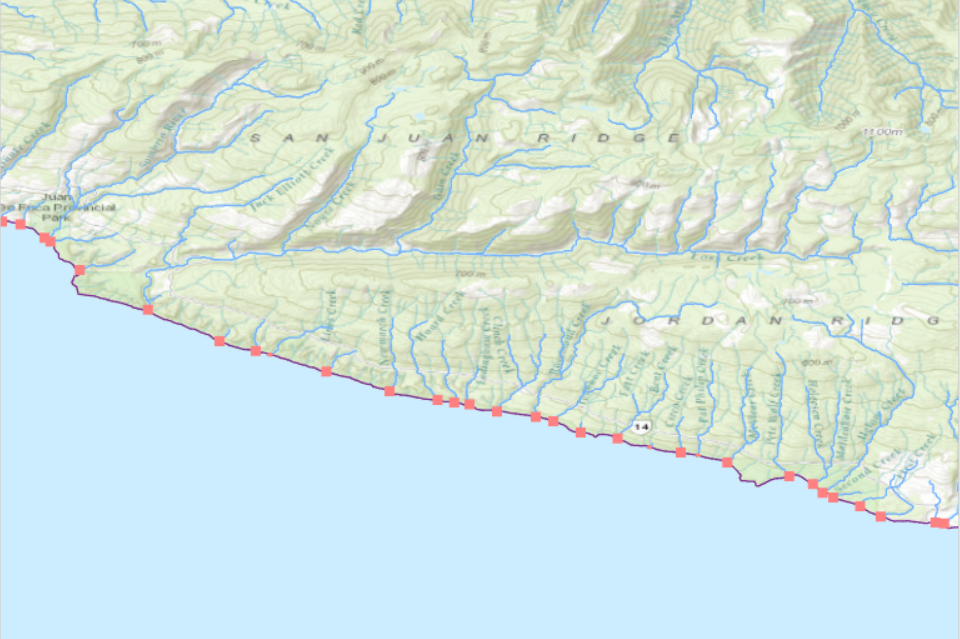
\includegraphics[width=1\linewidth]{images/02-ocean-stream-junctions}

\begin{center}\rule{0.5\linewidth}{0.5pt}\end{center}

\hypertarget{task-3-record-stream-attributes-with-linear-referencing}{%
\section*{Task 3: Record stream attributes with linear referencing}\label{task-3-record-stream-attributes-with-linear-referencing}}
\addcontentsline{toc}{section}{Task 3: Record stream attributes with linear referencing}

Now that we have stream routes, we can calculate some information that relate to salmon habitat. Water quality is important for salmon spawning habitat. Steeper gradients (slope) may be more susceptible to erosion that could be one proxy for lower water quality. In this task, you will practice extracting information about the streams and storing that information in the routes using linear referencing.

\textbf{Important:} Some of these operations can be computationally intensive because we will be dealing with up to 10\textsuperscript{5} features for the entire island. You can attempt to process the entire island, but ultimately you need to clip your stream routes to one of the conservation units (CU) for any of the three species of salmon for your report.

\textbf{Step 1:} Calculate the slope of the filled DEM using ``Percent rise'' as the output measurement and ``Planar'' as the Method.

\textbf{Step 2:} Now use the ``Extract by Mask'' tool to extract the slope raster by the mask of the stream links raster you created back in Task 1. This will produce a raster with slope values only where our streams exist.

\textbf{Step 3:} In British Columbia, stream gradients \textless{} 20\% are generally considered to be fish-bearing. Therefore, use the ``Reclassify'' tool to classify slopes \textless{} 20\% to a value of 1 and all other slopes to a value of 0 for the stream raster you created in the last step.

\textbf{Step 4:} Use the ``Stream to Feature'' tool to convert the classified slope raster to line features. Parameterize this tool as follows:

\begin{itemize}
\item
  Input stream raster is the classified slope raster you just made in step 3
\item
  Input flow direction raster is the original flow direction raster you made in Task 1
\item
  Name the output ``stream\_features\_slope\_classified''
\item
  \textbf{Uncheck} ``Simplify polygons''
\end{itemize}

Now you have another feature class of streams that should spatially match your stream routes, but these new polylines contain the gradient information. Now we will overlay this information with the routes. Open the attribute table of this layer, the field ``grid\_code'' stores the value of the reclassified slope raster for each stream segment.

\textbf{Step 5:} Use the ``Locate Features Along Routes'' tool to overlay the gradient information with the routes.

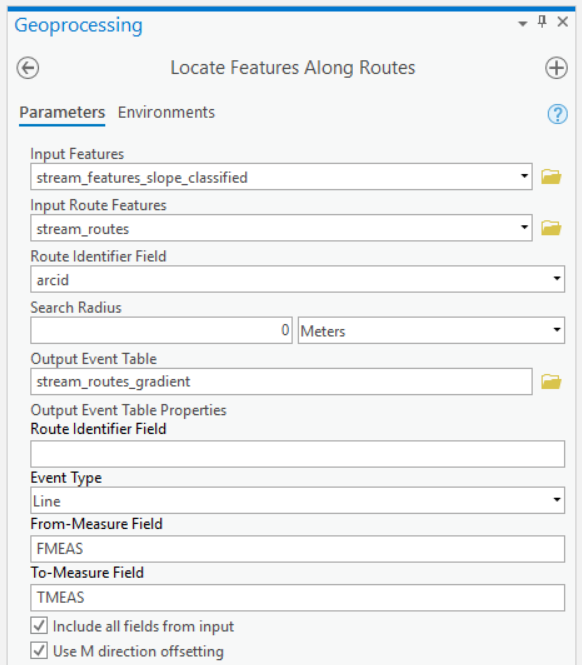
\includegraphics[width=0.75\linewidth]{images/02-locate-features-along-routes}

This will produce a route event table that should look something like this:

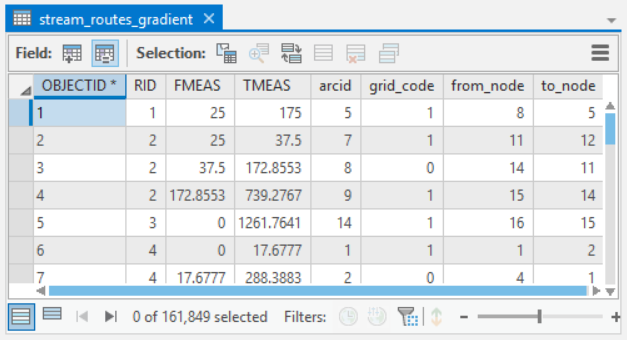
\includegraphics[width=0.75\linewidth]{images/02-stream-routes-gradient}

grid\_code in the event table represents the classified stream gradient (0 is ≥20\%, 1 is \textless20\%). Note that you have more records in this table than you have routes, because many routes are being segmented based on the gradient. Thus, you see repeating route id''s (RID).

Add a Short field to the event table called ``GRADIENT'' and calculate this field as !grid\_code! to transfer the grid\_code values to a more meaningful field name.

\textbf{Step 6:} Repeat steps 4 and 5 above for the stream order raster that you generated in Task 1. Ensure that the stream\_order raster is used as the ``Input stream raster'' and ``Simplify polygons'' is toggled off. In the end, you should have a second event table where the grid\_code (values between 1 and 6) indicates the stream order for each route. Again, add a Short field to the event table called ``SORDER'' and calculate this field as !grid\_code! to transfer the grid\_code values to a more meaningful field name.

\begin{center}\rule{0.5\linewidth}{0.5pt}\end{center}

\hypertarget{task-4-trace-the-network}{%
\section*{Task 4: Trace the network}\label{task-4-trace-the-network}}
\addcontentsline{toc}{section}{Task 4: Trace the network}

Now we can create a network that will allow us to trace the routes from the ocean to the dams. The goal of this task is to identify routes through the stream network that flow to the ocean and are unimpeded by dams. The following link provides more information about trace networks in ArcGIS Pro: \url{https://pro.arcgis.com/en/pro-app/latest/help/data/trace-network/what-is-a-trace-network-.htm}

The following steps will use the ``stream\_dams\_junction'', ``stream\_ocean\_junctions'' and the ``vancouver\_island\_stream\_routes'' layers. Before running the next steps save your ArcGIS Project. Ensure you have cleared any selected features from the map.

\textbf{Step 1:} Open the ``Create Trace Network'' tool:

\begin{itemize}
\item
  The Input Feature Dataset should point to your feature dataset in your geodatabase
\item
  Trace Network Name can be named ``stream\_trace\_network''
\item
  Input Junctions should contain both the ``stream\_dams\_junction'' and ``stream\_ocean\_junctions'' from the Topology geodatabase.
\item
  Input Edges should contain the clipped stream routes and set the Connectivity Policy to ``Complex edge''
\end{itemize}

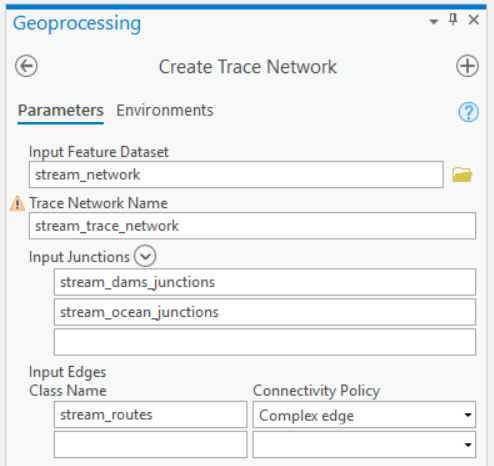
\includegraphics[width=0.5\linewidth]{images/02-create-trace-network}

\textbf{Step 2:} Run the ``Enable Network Topology'' tool on the trace network you just created.

\textbf{Step 3:} Run the ``Validate Network Topology'' tool on the trace network you just created. You might receive a warning: "A dirty area is not present within the specific extent." Ignore it.

\textbf{Step 4:} Open the ``Trace'' tool. This tool traces a path along a network the meets specified criteria. It also supports modelling barriers, so that the tracing terminates when a barrier feature is reached. Here is how we will parameterize this tool:

\begin{itemize}
\item
  Input Trace Network is the trace network that you created earlier
\item
  Trace Type is ``Connected''
\item
  Starting Points are the ``stream\_ocean\_junctions'' (make sure this is the layer stored in the Topology geodatabase)
\item
  Barriers are the ``stream\_dam\_junctions'' (make sure this is the layer stored in the Topology geodatabase)
\item
  Toggle on ``Include Barrier Features''
\item
  Toggle off ``Validate Consistency''
\item
  Toggle off ``Ignore Barriers at Starting Points''
\item
  Leave all Advanced Options as defaults
\end{itemize}

After the tool has finished running, toggle off the stream trace network and toggle on the stream routes layer (``vancouver\_island\_stream\_routes''). You should see some of the routes are now highlighted on your map.

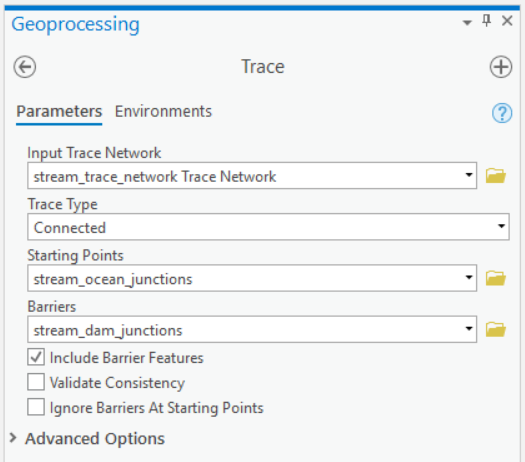
\includegraphics[width=0.5\linewidth]{images/02-trace}

\textbf{Step 5:} Add a Short field to the stream routes attribute table called ``REACHED''. Calculate this field with a value of ``1'' for the routes selected. Invert the selection and calculate the field again for the selected features with a value of ``0''. Finally, clear the selection and symbolize the routes based on the ``REACHED'' field. Congratulations! You have now modeled which route segments can be reached from the ocean and are not impeded by dams. Your stream\_routes should look something like this (blue = unimpeded streams, yellow = stream reaches that are impeded by a dam):

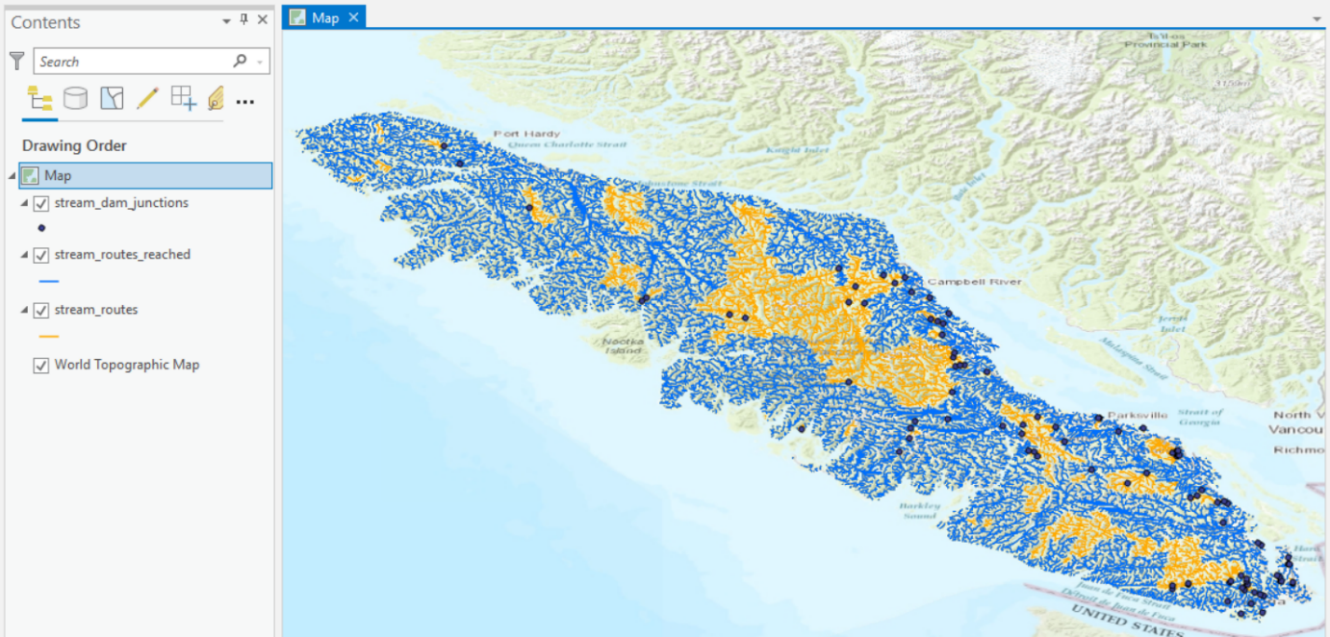
\includegraphics[width=1\linewidth]{images/02-traced-network}

\textbf{Important:} If your map looks significantly different from above, like most of the streams are impeded, then try these fixes:

\begin{itemize}
\item
  Zoom in closely to the ocean and dam junctions to ensure they are overlapping with the stream routes.
\item
  Apply a new topology rule that dam/ocean junctions must be coincident with the stream routes.
\item
  If there are any errors from above, then use the ``Snap'' tool to force the ocean and dam junctions to. The input features are the features that you want to move (snap), in this case the ocean and dam junction points. The type should be set to ``Edge'' and usually a distance of 25-30 meters is sufficient, but check the output
\item
  If you are still having trouble, try deleting the Trace Network from the feature dataset and rebuilding it (``Create Trace Network'' + ``Enable Network Topology'' + ``Validate Network Topology'').
\item
  If you are unable to delete the trace network, your geodatabase may be corrupt. Try creating a new geodatabase and import or re-create the important feature classes. Then, re-create the feature dataset and rebuild the trace network.
\end{itemize}

\begin{center}\rule{0.5\linewidth}{0.5pt}\end{center}

\hypertarget{task-5-overlay-and-query-the-network}{%
\section*{Task 5: Overlay and query the network}\label{task-5-overlay-and-query-the-network}}
\addcontentsline{toc}{section}{Task 5: Overlay and query the network}

Now you will practice doing an overlay with your route event tables to transfer all the attributes into a common linear referencing system. This will allow you to then query the network for stream segments that meet some basic conditions for salmon habitat.

\textbf{Step 1:} Parameterize the ``Overlay Route Events'' tool like below:

\begin{itemize}
\item
  Input Event Table is your classified gradient event table from Task 3
\item
  Overlay Event Table is the stream order event table from Task 3
\item
  From-Measure Field is FMEAS
\item
  To-Measure Field is TMEAS for both input event tables and the output event table
\item
  Type of Overlay is Intersect
\item
  Name the Output Event Table ``stream\_route\_overlay''
\item
  Leave the Route Identifier Field empty for the output, but ensure it is set to RID for both the input tables
\end{itemize}

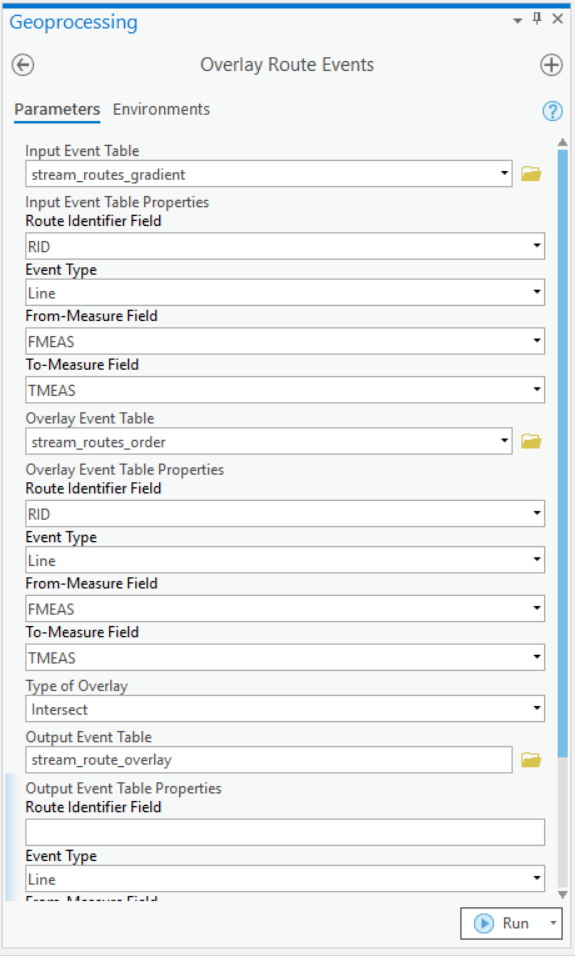
\includegraphics[width=0.5\linewidth]{images/02-overlay-route-events}

This will produce a new output event table that contains the intersection of stream gradient and stream order along the routes. As well, this event table should contain which routes can be reached from the ocean before running into a dam. Keep in mind that this is just a table, not a feature class. This is known as dynamic segmentation. Next we will add one last field, visualize the everything and do a simple query.

\textbf{Step 2:} Join the field ``REACHED'' from the original routes to the overlay event table you just created using the ``Join Field'' tool. The stream\_routes layer should be the layer with the REACHED field:

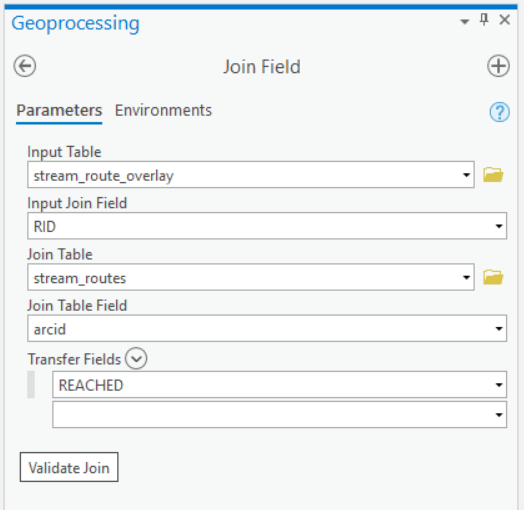
\includegraphics[width=0.5\linewidth]{images/02-join-field}

You should now have a table that has all the fields we need: SORDER, GRADIENT, and REACHED. (Note that some fields have been hidden from view in the table below.)

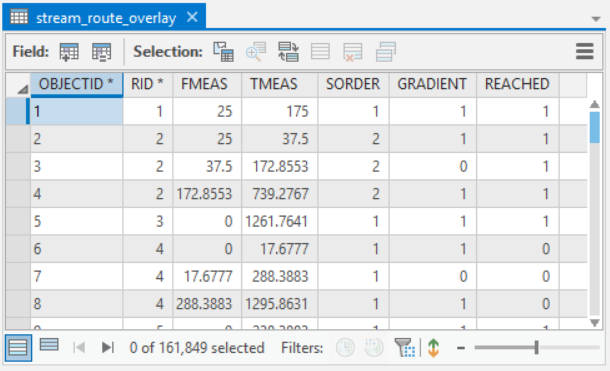
\includegraphics[width=1\linewidth]{images/02-stream-route-overlay}

\textbf{Step 3:} Use the ``Make Route Event Layer'' tool to convert the output event table to a feature class. Parameterize the tool as follows:

\begin{itemize}
\item
  Input route features will be the routes you originally created in Task 1
\item
  Route identifier field is ``arcid''
\item
  Input event table is the ``stream\_route\_overlay'' table that you created from step 1
\item
  From-measure field is ``FMEAS''
\item
  To-measure field is ``TMEAS''
\item
  Layer name or Table view is ``stream\_route\_overlay\_layer''
\end{itemize}

\textbf{Step 4:} Query the event layer from step 2 for stream segments with the following requirements:

\begin{itemize}
\item
  \ul{\textbf{Can}} be reached from the ocean
\item
  Is 1\textsuperscript{st} or 2\textsuperscript{nd} order stream
\item
  Has a gradient not steeper than 20\%
\end{itemize}

Export the selected features to a new feature class called ``accessible\_salmon\_habitat''.

\textbf{Step 5:} Repeat the query using the following requirements:

\begin{itemize}
\item
  \ul{\textbf{Cannot}} be reached from the ocean
\item
  Is 1\textsuperscript{st} or 2\textsuperscript{nd} order stream
\item
  Has a gradient not steeper than 20\%
\end{itemize}

Export the selected features to a new feature class called ``inaccessible\_salmon\_habitat''.

If everything goes \emph{swimmingly}, then the selected stream segments that meet the habitat criteria and can be reached from the ocean will look something like this:

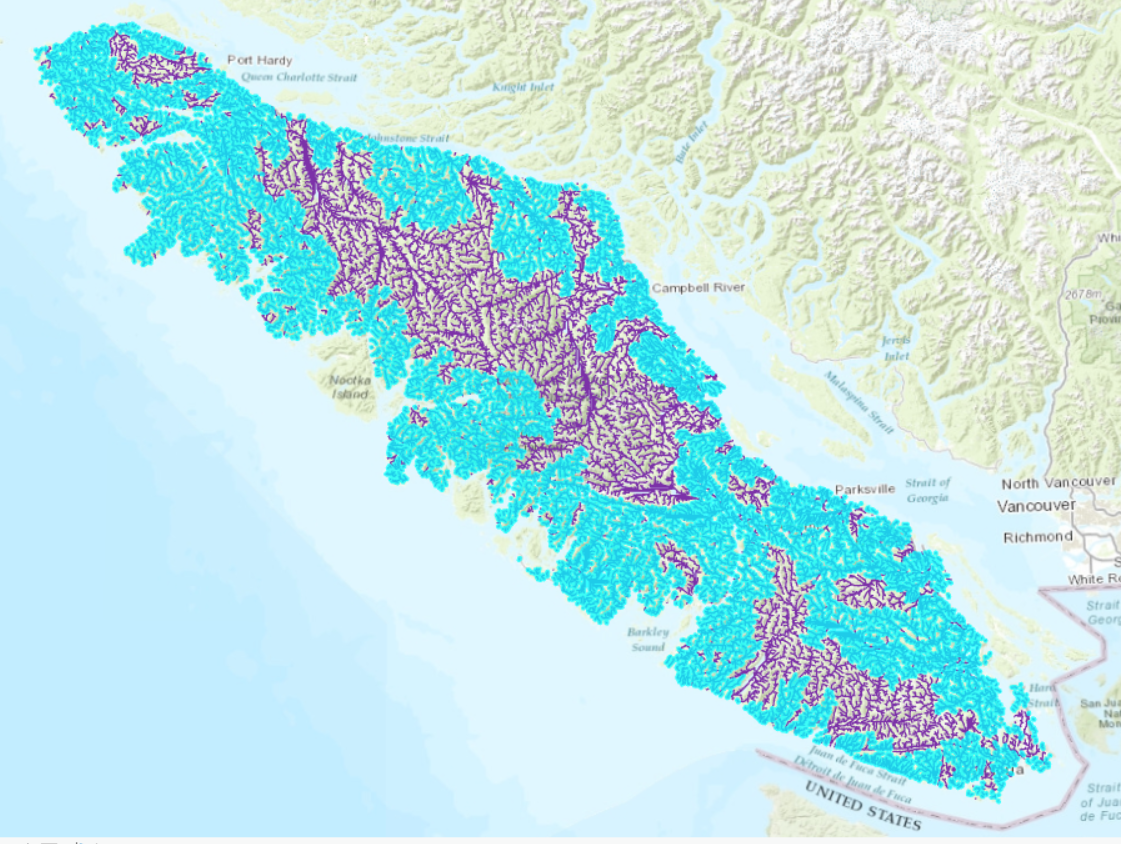
\includegraphics[width=1\linewidth]{images/02-selected-streams}

\textbf{For your final report, you will clip these layers to one of the salmon conservation units.}

\hypertarget{final-report}{%
\section*{Final Report}\label{final-report}}
\addcontentsline{toc}{section}{Final Report}

For your report, summarize your findings up through the final task. Comment on both small and large scale observations that you made throughout the process. Small scale observations would be investigating the behavior/structure of individual routes, while large scale observations would be the overall differences between total salmon habitat and habitat that can actually be reached from the ocean. Additionally, discuss any limitations to the analysis based on your observations and suggest how the modelling process might be improved further. Illustrate your findings with figures, maps, and tables as needed. You are only expected to comment on a single conservation unit, but you may also run the entire island if you feel ambitious.

Because we introduced so many tools and the lab is already process-intensive, there is no requirement to undertake additional analysis for another scenario. Instead, we are asking you to consider how you might model the other salmon habitat requirements laid out at the beginning of the lab. Give brief examples for how you would model at least three of the criteria that we did not consider in the lab (i.e., do not discuss stream order, stream gradient). Assume that you have access to any typical data source (e.g., LiDAR, optical satellite, RADAR, land inventory, gauge stations, weather stations, etc).

Finally, answer the following questions in your report:

\begin{itemize}
\tightlist
\item
  Zoom to Lake Cowichan. What is going on here? What could you do to automatically fix this for all large lakes?
\item
  How well do the streams you created line up with the mapped streams in the ArcGIS basemap?
\item
  How would you expect the stream network to change if you used a raster with a cell size of 5m or 100m?
\item
  How might additional topological errors and unidentified/unfilled sinks in the DEM impact your analysis?
\end{itemize}

\begin{center}\rule{0.5\linewidth}{0.5pt}\end{center}

\hypertarget{summary-1}{%
\section*{Summary}\label{summary-1}}
\addcontentsline{toc}{section}{Summary}

Would you have guessed that you could do all that analysis from a single DEM? That is the power of applying focal functions to the raster (flow direction, flow accumulation, slope) and deriving a network with topology. In this lab, we were principally concerned with events and attributes along the stream segments. Although we did not explicitly calculate connectivity measures, the connectivity of the network was implied through the modelling approach using flow direction from the filled DEM. If you attempted to perform this same analysis without the aid of a DEM, then you would need to take additional precautions to ensure that your polyline features have topological connectivity and valid junctions. Still, our approach using a DEM is prone to artifacts from the raster. Stream segments are limited to eight turning angles and the resolution of the DEM can impact stream attributes.

Return to the \protect\hyperlink{lab2-deliverables}{\textbf{Deliverables}} section to check off everything you need to submit for credit in the course management system.

\hypertarget{lidar-for-forest-management}{%
\chapter{Lidar for Forest Management}\label{lidar-for-forest-management}}

Written by
Nicholas Coops

\hypertarget{lab-overview-2}{%
\section*{Lab Overview}\label{lab-overview-2}}
\addcontentsline{toc}{section}{Lab Overview}

The aim of this lab is to use LiDAR data from the Malcolm Knapp Research Forest (MKRF) explore a discrete return LiDAR dataset and become familiar with basic functions in the R package lidR and .las data sets. You will create digital terrain models (DTMs), digital surface models (DSM), canopy height models (CHMs) and visualize the point clouds in R. Additionally, we will explore individual tree detection and examine how LiDAR can be used to model forest attributes.

\begin{center}\rule{0.5\linewidth}{0.5pt}\end{center}

\hypertarget{learning-objectives-2}{%
\section*{Learning Objectives}\label{learning-objectives-2}}
\addcontentsline{toc}{section}{Learning Objectives}

\begin{itemize}
\tightlist
\item
  Create a DEM from LiDAR point data in both 2D and 3D
\item
  Calculate meaningful metrics from points clouds
\item
  Apply an OLS model to predict forest forest attributes with LiDAR metrics
\item
  Practice variable selection in modeling
\item
  Apply individual tree detection using point and CHM to create a map of tall trees from a LiDAR point cloud
\end{itemize}

\begin{center}\rule{0.5\linewidth}{0.5pt}\end{center}

\hypertarget{lab3-deliverables}{%
\section*{Deliverables}\label{lab3-deliverables}}
\addcontentsline{toc}{section}{Deliverables}

Turn in the answers to the questions given in the lab on Canvas.

\begin{center}\rule{0.5\linewidth}{0.5pt}\end{center}

\hypertarget{data-2}{%
\section*{Data}\label{data-2}}
\addcontentsline{toc}{section}{Data}

We will be working with LiDAR data collected over the Malcolm Knapp Research Forest (MKRF) in Maple Ridge, BC. There are three files associated with this lab:

\begin{itemize}
\tightlist
\item
  MKRF\_Data\_Specifications.pdf: A document describing the LiDAR data collection
\item
  LAS folder: The LiDAR data files in .LAS format. .LAS is the standard file type for LiDAR data
\item
  MKRF\_Aerial\_Photo.tif: An orthophoto of our study area, which was collected at the same time as the LiDAR data
\item
  MKRF\_lidar: a single lidar file of the MKRF
\item
  Empty folders: you will save your outputs to these folders
\item
  Variety of CSVs used to create models
\item
  Lab6\_Script.r: A script to process .las files using R and the lidR library.
\end{itemize}

\begin{center}\rule{0.5\linewidth}{0.5pt}\end{center}

\hypertarget{software}{%
\section*{Software}\label{software}}
\addcontentsline{toc}{section}{Software}

\begin{itemize}
\tightlist
\item
  R/RStudio
\end{itemize}

For this lab you will need to download R and RStudio. Rstudio is an open source integrated development environment (IDE, think fancy notepad) for the R programing language. It includes a console, syntax editor for code execution and will generally improve your R programing experience. If you need to install \href{https://cran.rstudio.com/}{R} and \href{https://posit.co/download/rstudio-desktop/}{R studio} click the respective links or ask your TA. If you already have them installed on your computer continue to the next section of the lab.

\textbf{Warning:} This lab (and LiDAR processing in general) is computationally demanding. I have reduced the study area and used less rigorous algorithms to speed up processing time. Generally speaking a single line of code should not take longer than 5 minutes to run.

\begin{center}\rule{0.5\linewidth}{0.5pt}\end{center}

\hypertarget{lab-set-up}{%
\section*{Lab Set up}\label{lab-set-up}}
\addcontentsline{toc}{section}{Lab Set up}

For this lab we will use two R packages: lidR and tidyverse

LidR contains the functions used to process the lidar data, while tidyverse is a generic set of function to help with data wrangling and manipulation.

To run lines of code within Rstudio you can use \textbf{ctrl+enter}. This will run either the highlighted text or the line of code your cursor is on.

To begin open RStudio and check if the packages are installed

\begin{Shaded}
\begin{Highlighting}[]
\CommentTok{\#Install and/or load packages }

\CommentTok{\#install.packages("lidR")\# Run if not installed }
\CommentTok{\#install.packages("tidyverse")\# Run if not installed}

\FunctionTok{library}\NormalTok{(lidR)}
\FunctionTok{library}\NormalTok{(tidyverse)}
\end{Highlighting}
\end{Shaded}

Set your working directory to the folder that contains your Lab 3 data using the setwd() function. Doing so will save you time during file uploading/exporting throughout the lab. If you forget your working directory after it is set, you can type getwd() into the console and R will print it for you.

\begin{Shaded}
\begin{Highlighting}[]
\CommentTok{\# This is the only section of the lab you will need to fill out yourself. }
\CommentTok{\# It should look something like this setwd("C:/Users/Spencer/FRST538/Lab6/Data") but using the path for your computer }
\FunctionTok{setwd}\NormalTok{(}\StringTok{"C:/\{file\_path\}"}\NormalTok{)}
\end{Highlighting}
\end{Shaded}

\begin{center}\rule{0.5\linewidth}{0.5pt}\end{center}

\hypertarget{task-1-load-rgb-imagery}{%
\section*{Task 1: Load RGB Imagery}\label{task-1-load-rgb-imagery}}
\addcontentsline{toc}{section}{Task 1: Load RGB Imagery}

When working with any airborne spatial data, it is useful to examine an RGB photo of the study site (MKRF\_Aerial\_Photo.tif). Take time to locate different land cover features (roads, lakes, streams, etc.) and to understand how vegetation structures are distributed. Is there wall-to-wall forest at the site? Are there any cut-blocks or major roads that could act as reference points during processing? Will the location of water bodies compromise random plot selection?

For this lab, these considerations have already been made. At the very least, you can use the RGB image of Malcolm Knapp Research Forest (MKRF) to gain perspective of our study area. We will use the brick function from the package raster, which was loaded automatically when we loaded lidR. This function creates a RasterBrick object from a multi-layer (or band) file (Figure \ref{fig:03-rgb-malcolm-knapp}).

You can explore the details of any function that we use in this lab by typing a question mark \texttt{?} followed by the function name into the console: \texttt{?brick}. The information will appear in the Help pane of your RStudio interface.

Once the RasterBrick has been read into R, we will explore the objects structure using the \texttt{str()} function and plot the RGB image using the plot function.

\begin{Shaded}
\begin{Highlighting}[]
\CommentTok{\#Load RGB image and explore structure}
\NormalTok{rgb\_mkrf }\OtherTok{\textless{}{-}} \FunctionTok{brick}\NormalTok{(}\StringTok{\textquotesingle{}Aerial\_Photo/MKRF\_Aerial\_Photo.tif\textquotesingle{}}\NormalTok{)}
\FunctionTok{str}\NormalTok{(rgb\_mkrf) }
\FunctionTok{plotRGB}\NormalTok{(rgb\_mkrf)}
\end{Highlighting}
\end{Shaded}

\begin{figure}

{\centering 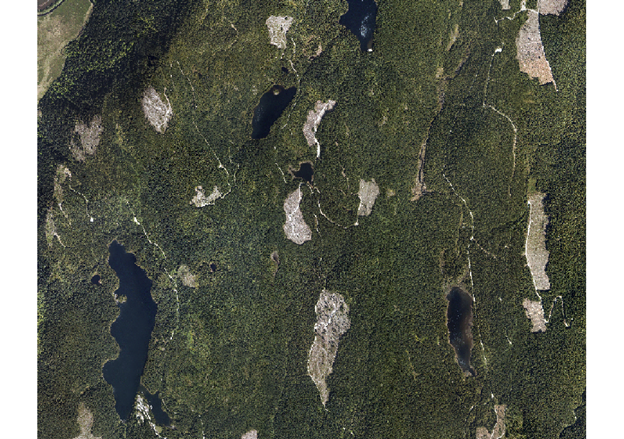
\includegraphics[width=1\linewidth]{images/03-rgb-malcolm-knapp} 

}

\caption{RGB image of the Malcolm Knapp Research Forest}\label{fig:03-rgb-malcolm-knapp}
\end{figure}

\begin{center}\rule{0.5\linewidth}{0.5pt}\end{center}

\hypertarget{task-2-load-and-explore-the-lidar-data}{%
\section*{Task 2: Load and Explore the LiDAR Data}\label{task-2-load-and-explore-the-lidar-data}}
\addcontentsline{toc}{section}{Task 2: Load and Explore the LiDAR Data}

First, we need to load the file MKRF\_lidar.las from your /Data folder. This file contains the lidar data you will need to complete this section of the lab. We will use the function \texttt{readLAS} to load the .las file. Once the file is loaded it should appear in your Environment as a `Large LAS'. It is best practice to use the function \texttt{lascheck} to conduct a deep inspection of a LAS object. This function will print a report for you to examine.

You can explore the structure of objects in your Environment using the \texttt{str()} base function in the Console. You can also explore the contents of a single column within the object by typing the objects name followed by a dollar sign and the column name: \texttt{object\$column}.

\emph{HINT: If you wish to learn the details of any function associated with your loaded packages, you can type a question mark followed by the functions name: \texttt{?function\_name}}

\begin{Shaded}
\begin{Highlighting}[]
\CommentTok{\#Load lidar data}
\NormalTok{las\_mkrf }\OtherTok{\textless{}{-}} \FunctionTok{readLAS}\NormalTok{(}\StringTok{"./MKRF\_lidar.las"}\NormalTok{) }\CommentTok{\#read the specified .las file  }
\FunctionTok{las\_check}\NormalTok{(las\_mkrf) }\CommentTok{\#check the LAS object}
\FunctionTok{str}\NormalTok{(las\_mkrf) }\CommentTok{\#compactly display the internal structure of las\_mkrf}
\FunctionTok{print}\NormalTok{(las\_mkrf)}
\end{Highlighting}
\end{Shaded}

\hypertarget{q1-examine-the-lascheck-output.-is-the-data-normalized-has-a-ground-classification-been-completed-already}{%
\paragraph*{Q1: Examine the lascheck output. Is the data normalized? Has a ground classification been completed already?}\label{q1-examine-the-lascheck-output.-is-the-data-normalized-has-a-ground-classification-been-completed-already}}
\addcontentsline{toc}{paragraph}{Q1: Examine the lascheck output. Is the data normalized? Has a ground classification been completed already?}

\hypertarget{q2-examine-the-output-of-str.-how-many-first-returns-are-there-what-is-the-maximum-z-value}{%
\paragraph*{Q2: Examine the output of str(). How many first returns are there? What is the maximum z value?}\label{q2-examine-the-output-of-str.-how-many-first-returns-are-there-what-is-the-maximum-z-value}}
\addcontentsline{toc}{paragraph}{Q2: Examine the output of str(). How many first returns are there? What is the maximum z value?}

\hypertarget{q3-examine-the-output-of-print.-what-is-the-density-of-this-data-is-that-high-low-or-somewhere-in-the-middle}{%
\paragraph*{Q3: Examine the output of print(). What is the density of this data? Is that high, low, or somewhere in the middle?}\label{q3-examine-the-output-of-print.-what-is-the-density-of-this-data-is-that-high-low-or-somewhere-in-the-middle}}
\addcontentsline{toc}{paragraph}{Q3: Examine the output of print(). What is the density of this data? Is that high, low, or somewhere in the middle?}

Upon exploring the lascheck output you will notice that there are some duplicated points. This is not a problem for our analyses, but it is worth noting. For example, the statement: There were 6 degenerated ground points. Some X Y coordinates were repeated but with different Z coordinates means that multiple pulses measured the same location and returned different Z, or elevation, coordinates. This could be caused by overlapping flight paths or pre-processing errors, but lidR has the capacity to deal with these issue. Overall, our lidar data looks good. Before moving on let us remove the duplicated points.

\begin{Shaded}
\begin{Highlighting}[]
\CommentTok{\#remove duplicated Z (eleavation) points}
\NormalTok{las\_mkrf }\OtherTok{\textless{}{-}} \FunctionTok{filter\_duplicates}\NormalTok{(las\_mkrf) }\CommentTok{\#remove the duplicated points}
\CommentTok{\#confirm duplicates removed}
\FunctionTok{las\_check}\NormalTok{(las\_mkrf) }\CommentTok{\#run lascheck a second time to ensure duplicates removed}
\end{Highlighting}
\end{Shaded}

Now that we have a general understanding of our lidar data, it is time to start visualizing! We will explore 2D and 3D plots of our data to gain an even deeper understanding of our study site before undergoing some basic manipulation.

First, we will visualize the density of lidar points across our site. You will notice that some areas have a higher density than others. This is likely due to the flight path of the aircraft that collected our data and probably causes some of the duplicated points that were highlighted by \texttt{lascheck}. Next, we will plot las\_mkrf in 3D using the plot function. In lidR, this function can produce plots

in 2D or 3D, depending on structure of the input object. LASobjects are plotted in 3D, while Raster objects are 2D.

\begin{Shaded}
\begin{Highlighting}[]
\CommentTok{\#Visualize point density }
\NormalTok{density\_mkrf }\OtherTok{\textless{}{-}} \FunctionTok{grid\_density}\NormalTok{(las\_mkrf, }\AttributeTok{res =} \DecValTok{2}\NormalTok{) }\CommentTok{\#create a map of the point density}
\FunctionTok{plot}\NormalTok{(density\_mkrf) }

\CommentTok{\#Visualize las\_mkrf in 3D }
\FunctionTok{plot}\NormalTok{(las\_mkrf)}
\end{Highlighting}
\end{Shaded}

Wonderful! We can now explore lidar data in 3D by clicking and scrolling through the RGL plot. Due to the size of the file this exploration may be relatively slow (Figure \ref{fig:03-rgl-plot}).

\begin{center}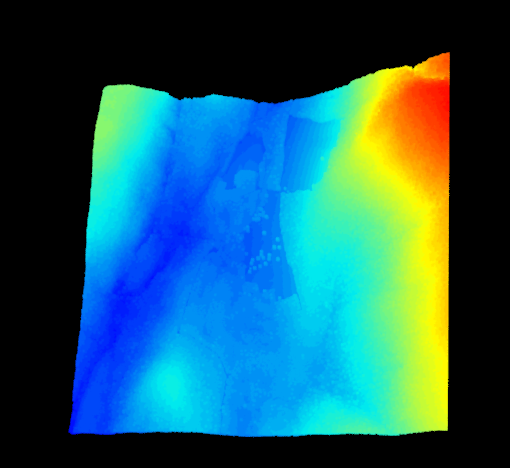
\includegraphics[width=1\linewidth]{images/03-rgl-plot} \end{center}

\begin{center}\rule{0.5\linewidth}{0.5pt}\end{center}

\hypertarget{task-3-read-multiple-las-files-into-lascatolog-object}{%
\section*{Task 3: Read Multiple LAS Files into LAScatolog object}\label{task-3-read-multiple-las-files-into-lascatolog-object}}
\addcontentsline{toc}{section}{Task 3: Read Multiple LAS Files into LAScatolog object}

Once you have a basic understanding of the study area, it is time to load your lidar data. The file type used in this course is LAS, which is an industry standard format for storing lidar data. In the future, you may also work with other file formats, such as LAZ. You can explore the differences between these formats \href{https://rapidlasso.de/five-myths-about-las-laz-and-optimized-las/}{online}.

In the last task, we loaded a single LAS object and plotted it. For the remainder of this lab, we will load 20 tiles collected over MKRF into a LAScatalog object. This will enable us to manage and process our entire data set as one object, rather than 20 separate files. We can use lascheck to perform a deep inspection of the LASCatalog object or use \texttt{summary()} for a more succinct report.

We can also plot a LAScatalog object to observe how our tiles are arranged. Since the LASCAtalog object is a SpatialPolygonsDataFrame, it is possible to use the \texttt{spplot} function to visualize certain characteristics of our data. For example, the line \texttt{spplot(cat\_mkrf,\ "Min.Z")} will plot catalog and color each tile based on it's lowest elevation (Z) value (Figure \ref{fig:03-rgl-plot}).

\begin{Shaded}
\begin{Highlighting}[]
\CommentTok{\#Create LAScatalog object from MKRF las tiles}
\NormalTok{cat\_mkrf }\OtherTok{\textless{}{-}} \FunctionTok{readLAScatalog}\NormalTok{(}\StringTok{"LAS"}\NormalTok{)}
\FunctionTok{las\_check}\NormalTok{(cat\_mkrf)}
\FunctionTok{summary}\NormalTok{(cat\_mkrf)}
\FunctionTok{plot}\NormalTok{(cat\_mkrf)}
\end{Highlighting}
\end{Shaded}

Notice that there are overlapping tiles. This indicates that there may be duplicate points within our data. We can confirm this by applying the \texttt{lascheck} function to a single tile.

\begin{Shaded}
\begin{Highlighting}[]
\CommentTok{\#Examine single .las tile to determine duplication}
\NormalTok{tile\_1\_mkrf }\OtherTok{\textless{}{-}} \FunctionTok{readLAS}\NormalTok{(}\StringTok{"LAS/MKRF\_Tile1.las"}\NormalTok{)}
\FunctionTok{lascheck}\NormalTok{(tile\_1\_mkrf)}
\end{Highlighting}
\end{Shaded}

It appears that there are 421 duplicate points. These may impact both the accuracy of our analysis and the processing speed. Let us remove them using the \texttt{filter\_duplicates} function and store the filtered tiles in a new folder named `Filtered' (this folder has already been created for you). Once complete, confirm that the duplicates were removed.

\begin{Shaded}
\begin{Highlighting}[]
\CommentTok{\#Set the output directory for the filtered .las data}
\NormalTok{work\_dir }\OtherTok{=} \FunctionTok{getwd}\NormalTok{() }\CommentTok{\#create a filepath to your working directory}
\FunctionTok{opt\_output\_files}\NormalTok{(cat\_mkrf) }\OtherTok{\textless{}{-}} \FunctionTok{paste}\NormalTok{(work\_dir, }\StringTok{"/Filtered/filtered\_mkrf\_\{ID\}"}\NormalTok{, }\AttributeTok{sep =} \StringTok{""}\NormalTok{)}\CommentTok{\#location to store duplicate points}
\NormalTok{cat\_mkrf }\OtherTok{\textless{}{-}} \FunctionTok{filter\_duplicates}\NormalTok{(cat\_mkrf) }\CommentTok{\#remove duplicate points and speed up processing}

\CommentTok{\#confirm that duplicates were removed for Tile 1}
\NormalTok{filtered\_t1\_mkrf }\OtherTok{\textless{}{-}} \FunctionTok{readLAS}\NormalTok{(}\StringTok{"Filtered/filtered\_mkrf\_1.las"}\NormalTok{) }\CommentTok{\#load from stored file}
\FunctionTok{lascheck}\NormalTok{(filtered\_t1\_mkrf)}
\end{Highlighting}
\end{Shaded}

Success! We can now proceed with our analysis. Let us read all filtered LAS data into a catalog and perform the usual checks.

\begin{Shaded}
\begin{Highlighting}[]
\CommentTok{\#read filtered .las into LAScatalog}
\NormalTok{filtered\_cat\_mkrf }\OtherTok{\textless{}{-}} \FunctionTok{readLAScatalog}\NormalTok{(}\StringTok{"Filtered"}\NormalTok{)}
\FunctionTok{summary}\NormalTok{(filtered\_cat\_mkrf)}
\FunctionTok{plot}\NormalTok{(filtered\_cat\_mkrf)}
\FunctionTok{spplot}\NormalTok{(filtered\_cat\_mkrf, }\StringTok{"Min.Z"}\NormalTok{)}
\end{Highlighting}
\end{Shaded}

\begin{center}\rule{0.5\linewidth}{0.5pt}\end{center}

\hypertarget{task-4-create-digital-elevation-model-dem}{%
\section*{Task 4: Create Digital Elevation Model (DEM)}\label{task-4-create-digital-elevation-model-dem}}
\addcontentsline{toc}{section}{Task 4: Create Digital Elevation Model (DEM)}

Now that we have practiced some of the basic visualization, reading, and cleaning techniques on raw lidar data it is time to move onto processing. The first thing we will do is create a digital elevation model (DEM). A DEM represents the Earth's surface without vegetation, which we will refer to as ``ground''. Although this seems like an intuitive statement, there is the potential for logs, rocks and other non-soil objects to be included as ground points. These won't cause issues for our analyses, but it is important to use precise language when working with common words like ``ground''. Never assume that your definition of something is a global truth. It is also important to consider that a DEM can also be referred to as a digital terrain model (DTM). Take time to understand that both terms refer to a surface model of only ground points. Instructors/colleagues could use DEM and DTM interchangeably.

We will create and visualize a DEM in both 2D and 3D. The 3D version will be created by filtering out all points that are not classified as ground (Classification: 2). For the 2D DEM, we will use the \texttt{grid\_terrain} function on our LidR catalogue. This function enables the user to select the output resolution and the algorithm that computes spatial interpolation. It is recommended that you take time to understand the three algorithms in highlighted in the \texttt{grid\_terrain} `Help' file.

\begin{Shaded}
\begin{Highlighting}[]
\CommentTok{\#DEM}
\CommentTok{\#3D}
\NormalTok{dem\_3D\_mkrf }\OtherTok{\textless{}{-}} \FunctionTok{filter\_poi}\NormalTok{(las\_mkrf, Classification }\SpecialCharTok{==} \DecValTok{2}\NormalTok{)}
\FunctionTok{plot}\NormalTok{(dem\_3D\_mkrf) }\CommentTok{\#zoom in to notice no trees}
\FunctionTok{plot}\NormalTok{(las\_mkrf) }\CommentTok{\# compare to dem\_3dmkrf}
\CommentTok{\#demCatalog}
\NormalTok{dem\_allLAS\_mkrf }\OtherTok{\textless{}{-}} \FunctionTok{grid\_terrain}\NormalTok{(filtered\_cat\_mkrf, }\DecValTok{2}\NormalTok{, }\FunctionTok{tin}\NormalTok{()) }\CommentTok{\#why use this method? check warnings: why might points get degenerated DON\textquotesingle{}T PANIC AT \textquotesingle{}WARNING\textquotesingle{}}
\CommentTok{\# create Colour ramp for visualization }
\NormalTok{col\_1 }\OtherTok{\textless{}{-}} \FunctionTok{height.colors}\NormalTok{(}\DecValTok{50}\NormalTok{)}
\FunctionTok{plot}\NormalTok{(dem\_allLAS\_mkrf, }\AttributeTok{col =}\NormalTok{ col\_1)}
\end{Highlighting}
\end{Shaded}

\hypertarget{screenshot-1-submit-the-output-of-this-plot-as-a-screenshot.}{%
\paragraph*{Screenshot 1: Submit the output of this plot() as a screenshot.}\label{screenshot-1-submit-the-output-of-this-plot-as-a-screenshot.}}
\addcontentsline{toc}{paragraph}{Screenshot 1: Submit the output of this plot() as a screenshot.}

With the DEM complete we can normalize our LAScatalog. Each tile will be normalized separately, which means there will be one normalized output tile for each input. lidR requires an output directory to be specified. A folder named `Normalized' has already been created for you. Once the output file directory is set we will use \texttt{lasnormalize} to conduct the normalization of all our MKRF lidar tiles.

\begin{Shaded}
\begin{Highlighting}[]
\CommentTok{\#Normalize catalog with DEM}
\NormalTok{norm\_tiles\_mkrf }\OtherTok{\textless{}{-}} \FunctionTok{lasnormalize}\NormalTok{(filtered\_cat\_mkrf, dem\_allLAS\_mkrf)}

\CommentTok{\#define LAScatalog engine options}
\FunctionTok{opt\_output\_files}\NormalTok{(filtered\_cat\_mkrf) }\OtherTok{\textless{}{-}} \FunctionTok{paste}\NormalTok{(work\_dir, }\StringTok{"/Normalized/norm\_mkrf\_\{ID\}"}\NormalTok{, }\AttributeTok{sep =} \StringTok{""}\NormalTok{)}

\CommentTok{\#normalize all tiles in cat\_mkrf with the DEM }
\NormalTok{norm\_tiles\_mkrf }\OtherTok{\textless{}{-}} \FunctionTok{normalize\_height}\NormalTok{(filtered\_cat\_mkrf, dem\_allLAS\_mkrf) }\CommentTok{\#check your folder when complete }

\CommentTok{\#check to see if the normalization worked}
\NormalTok{norm\_mkrf\_1 }\OtherTok{\textless{}{-}} \FunctionTok{readLAS}\NormalTok{(}\StringTok{"Normalized/norm\_mkrf\_1.las"}\NormalTok{)}
\FunctionTok{plot}\NormalTok{(norm\_mkrf\_1) }
\end{Highlighting}
\end{Shaded}

Explore the 3D rgl plot that is produced by the last line in the above code block (Figure \ref{fig:03-normalized-tile-mkrf}). Does anything look abnormal to you?

\begin{figure}

{\centering 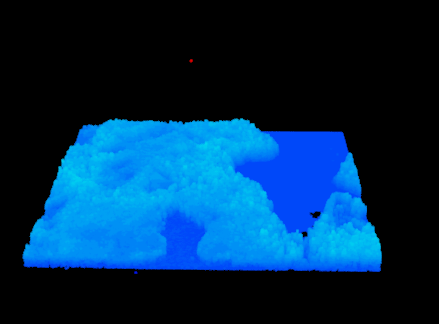
\includegraphics[width=1\linewidth]{images/03-normalized-tile-mkrf} 

}

\caption{Normalized tile 1 from MKRF.}\label{fig:03-normalized-tile-mkrf}
\end{figure}

\hypertarget{q4-there-appears-to-be-an-outlying-data-point-located-high-above-the-others.-explain-why-this-would-cause-issues-during-our-processing-and-an-example-of-what-would-cause-this-outlier.}{%
\paragraph*{Q4: There appears to be an outlying data point located high above the others. Explain why this would cause issues during our processing and an example of what would cause this outlier.}\label{q4-there-appears-to-be-an-outlying-data-point-located-high-above-the-others.-explain-why-this-would-cause-issues-during-our-processing-and-an-example-of-what-would-cause-this-outlier.}}
\addcontentsline{toc}{paragraph}{Q4: There appears to be an outlying data point located high above the others. Explain why this would cause issues during our processing and an example of what would cause this outlier.}

\begin{center}\rule{0.5\linewidth}{0.5pt}\end{center}

\hypertarget{task-5-create-a-canopy-height-model}{%
\section*{Task 5: Create a Canopy Height Model}\label{task-5-create-a-canopy-height-model}}
\addcontentsline{toc}{section}{Task 5: Create a Canopy Height Model}

We can explore the effect of this outlier by generating a canopy height model (CHM) with the grid\_canopy function. Mathematically, a CHM is simply the DEM (or DTM, remember these terms are interchangeable!) subtracted from the DSM. This subtraction can be called `normalization', differing from the normalization conducted using \texttt{lasnormalize} in the sense that the output is 2D. The CHM is an important surface model as it allows us to analyze objects above a common ground value (0m). This 2D output should have a maximum height around that of the highest tree on site (\textasciitilde{} 60m).

The \texttt{grid\_canopy} function is used to generate CHMs, which has three user defined arguments. The first, \texttt{las} refers to the input data (LAS or LAScatalog). The second, \texttt{res} refers to the spatial resolution. The third argument, \texttt{algorithm} specifies the algorithm that will be used to compute the digital surface model. There are three algorithms compatible with grid\_canopy:

\texttt{p2r} is a point-to-raster method. It returns the maximum height value of the point cloud for each area, which is defined by the spatial resolution. This is a relatively fast algorithm, but can generate `pits', or areas of `NoData' in the CHM where there are no returns present. You can add a subcircle argument within the p2r algorithm to try and remove pits. This method replaces each lidar point with a disk of a specified size and increases return coverage. If you use this method, be aware that issues related to computation speed may arise.

\texttt{dsmtin} is a triangulation-based method that creates a triangular irregular network (TIN) by interpolating only the first returns before generating a 2D grid. This method eliminates empty pixels, but can still generate pits within crowns as some first returns inevitably reach the ground.

\texttt{pitfree} is a triangulation-based method that conducts multiple triangulations at various heights. Developed by Khosravipour et al.~(2014), the pitfree algorithm ensure there are no empty cells or deep pits. Shallow pits may remain, but can be removed by adding a subcircle argument. Although the most sophisticated, this algorithm is computationally intense.

Since we know that our lidar data has 3.1 returns · m\textsuperscript{-2}, we can assume that a spatial resolution of 2 m will ensure that every cell in our raster contains at least one return. This, along with the advantage of quick processing (\textasciitilde1 min for entire site), allows us to use the stock \texttt{p2r} algorithm without worrying about pits. Feel free to use \texttt{dsmtin()} (\textasciitilde5 min) or \texttt{pitfree()} (\textasciitilde10 min) for the following steps, just ensure you annotate your code accordingly.

\begin{Shaded}
\begin{Highlighting}[]
\CommentTok{\#Create CHM for normalized Tile 1}
\NormalTok{chm\_mkrf\_1 }\OtherTok{\textless{}{-}} \FunctionTok{grid\_canopy}\NormalTok{(norm\_mkrf\_1, }\DecValTok{2}\NormalTok{, }\FunctionTok{p2r}\NormalTok{()) }\CommentTok{\#las, resolution, algorithm}
\FunctionTok{plot}\NormalTok{(chm\_mkrf\_1, }\AttributeTok{col =}\NormalTok{ col\_1) }\CommentTok{\#plot in 2D}
\FunctionTok{plot\_dtm3d}\NormalTok{(chm\_mkrf\_1) }\CommentTok{\#plot in 3D}
\end{Highlighting}
\end{Shaded}

It is clear that the normalization was not perfect as the maximum height of the CHM is well above our expected maximum height. This issue is caused by the outlier visible in the 3D plot. It also looks like there are some points below 0m. To remedy these issues, we can use the LAScatalog options engine to filter out data points below 0 m and above 65 m.

\begin{Shaded}
\begin{Highlighting}[]
\NormalTok{LAScatalog options engine to filter out data points below 0m and above 65m.}
\CommentTok{\#read normalized las into catalog to continue processing}
\NormalTok{norm\_cat\_mkrf }\OtherTok{\textless{}{-}} \FunctionTok{readLAScatalog}\NormalTok{(}\StringTok{"Normalized"}\NormalTok{)}

\CommentTok{\#add LAScatalog enginge option to filter undersired data points}
\FunctionTok{opt\_filter}\NormalTok{(norm\_cat\_mkrf) }\OtherTok{\textless{}{-}} \StringTok{\textquotesingle{}{-}drop\_z\_below 0 {-}drop\_z\_above 65\textquotesingle{}}

\CommentTok{\#ensure the entire study area was processed}
\FunctionTok{plot}\NormalTok{(norm\_cat\_mkrf)}
\FunctionTok{summary}\NormalTok{(norm\_cat\_mkrf)}
\end{Highlighting}
\end{Shaded}

It seems like all of the normalized LAS files were loaded correctly, but we still need to confirm that the outliers were removed by the filter we applied. To do this we will create another CHM. Instead of making the CHM for Tile 1, we will create a CHM for the entire site.

\begin{Shaded}
\begin{Highlighting}[]
\CommentTok{\#Create CHM for all normalized MKRF Tiles}
\NormalTok{chm\_mkrf }\OtherTok{\textless{}{-}} \FunctionTok{grid\_canopy}\NormalTok{(norm\_cat\_mkrf, }\DecValTok{2}\NormalTok{, }\FunctionTok{p2r}\NormalTok{()) }
\FunctionTok{plot}\NormalTok{(chm\_mkrf, }\AttributeTok{col =}\NormalTok{ col\_1) }\CommentTok{\#plot in 2D}
\CommentTok{\#plot\_dtm3d(chm\_mkrf) \#plot in 3D *DON\textquotesingle{}T RUN IF COMPUTER IS SLOW*}
\end{Highlighting}
\end{Shaded}

Excellent! The heights in our CHM are as expected. If you are interested in exploring how the CHM relates to the RGB image of the area, please compare the two now.

\hypertarget{screenshot-2-include-an-image-of-your-chm.}{%
\paragraph*{Screenshot 2: Include an image of your CHM.}\label{screenshot-2-include-an-image-of-your-chm.}}
\addcontentsline{toc}{paragraph}{Screenshot 2: Include an image of your CHM.}

\hypertarget{q5.-what-do-you-think-the-large-empty-locations-in-the-chm-represent}{%
\paragraph*{Q5. What do you think the large empty locations in the CHM represent?}\label{q5.-what-do-you-think-the-large-empty-locations-in-the-chm-represent}}
\addcontentsline{toc}{paragraph}{Q5. What do you think the large empty locations in the CHM represent?}

\begin{center}\rule{0.5\linewidth}{0.5pt}\end{center}

\hypertarget{task-6-extract-metrics-from-the-point-clouds}{%
\section*{Task 6: Extract Metrics From the Point Clouds}\label{task-6-extract-metrics-from-the-point-clouds}}
\addcontentsline{toc}{section}{Task 6: Extract Metrics From the Point Clouds}

Now that we have confirmed that our filter works at the catalog level, it is time to extract some plots. First, let us extract a single plot. We use the lasclip function to do this. Specifically, we will use lasclipCircle to extract circular plots from our lidar data. Check out the details of this function in the lidR documentation provided at the start of the lab. We will extract a plot with the following characteristics:

\textbf{X = 530118.9}

\textbf{Y = 5462882.0}

\textbf{Radius = 25}

\begin{Shaded}
\begin{Highlighting}[]
\CommentTok{\#Extract single plot}
\NormalTok{single\_plot\_mkrf }\OtherTok{\textless{}{-}} \FunctionTok{clip\_circle}\NormalTok{(norm\_cat\_mkrf, }\FloatTok{530118.9}\NormalTok{, }\FloatTok{5462882.0}\NormalTok{, }\DecValTok{25}\NormalTok{)}
\FunctionTok{plot}\NormalTok{(single\_plot\_mkrf) }
\end{Highlighting}
\end{Shaded}

Now we will extract multiple plots using a for loop. The location of each plots is provided in the `Plot\_Table.csv' within the `/Plots' folder of your lab data. Plot radii should be 30 m. The for loop is annotated for you so you can understand what each line of code is doing.

\begin{Shaded}
\begin{Highlighting}[]
\NormalTok{plot\_table }\OtherTok{\textless{}{-}} \FunctionTok{read\_csv}\NormalTok{(}\StringTok{"Plots/Plot\_Table.csv"}\NormalTok{)}
\NormalTok{radius }\OtherTok{\textless{}{-}} \DecValTok{30} \CommentTok{\#the radius for lasclipCircle()}
\ControlFlowTok{for}\NormalTok{(i }\ControlFlowTok{in} \DecValTok{1}\SpecialCharTok{:}\FunctionTok{nrow}\NormalTok{(plot\_table))\{ }\CommentTok{\#run the loop until i = the number of rows in \textquotesingle{}plot\_table\textquotesingle{} (20)}
\NormalTok{  plot\_cent }\OtherTok{\textless{}{-}} \FunctionTok{c}\NormalTok{(plot\_table}\SpecialCharTok{$}\NormalTok{X[i], plot\_table}\SpecialCharTok{$}\NormalTok{Y[i]) }\CommentTok{\#extract plot center}
\NormalTok{  plot\_las }\OtherTok{\textless{}{-}} \FunctionTok{clip\_circle}\NormalTok{(norm\_cat\_mkrf, plot\_cent[}\DecValTok{1}\NormalTok{], plot\_cent[}\DecValTok{2}\NormalTok{], radius) }\CommentTok{\#clip plot from norm\_cat\_las}
\NormalTok{  output\_file }\OtherTok{\textless{}{-}} \FunctionTok{paste}\NormalTok{(}\StringTok{"Plots/MKRF\_Plot\_"}\NormalTok{, i, }\StringTok{".las"}\NormalTok{, }\AttributeTok{sep =} \StringTok{""}\NormalTok{) }\CommentTok{\#output directory as string}
  \FunctionTok{writeLAS}\NormalTok{(}\FunctionTok{assign}\NormalTok{(}\FunctionTok{paste}\NormalTok{(}\StringTok{"MKRF\_Plot\_"}\NormalTok{, i, }\AttributeTok{sep =} \StringTok{""}\NormalTok{), plot\_las), output\_file) }\CommentTok{\#write\textquotesingle{}MKRF\_Plot\_i\textquotesingle{} to output dir.}
\NormalTok{\}}
\end{Highlighting}
\end{Shaded}

At this point, you can explore individual plots in 3D, which should be loaded in your Environment, using \texttt{plot()}.

Now that we have extracted our plots it is time to compute some standard cloud metrics. To do this, we will need to analyze each plot individually. We also need to make sure that we are only including the first returns. This will ensure our metrics do not include points that have been scattered throughout the canopy. Let's also remove all points below 2 m, as objects below this height could be non-tree (shrubs, fallen logs, etc.). We do not need to worry about outliers as we removed them during the normalization process. Explore the Console output of the line plot\_1\_metrics for a brief overview of the metrics being created.

\begin{Shaded}
\begin{Highlighting}[]
\CommentTok{\#Calculate cloud metrics for all plots}
\CommentTok{\#there are special considerations: only first returns between 2m and 65m}
\CommentTok{\#create empty dataframe}
\NormalTok{mkrf\_plot\_metrics }\OtherTok{\textless{}{-}} \FunctionTok{data.frame}\NormalTok{() }

\CommentTok{\#For loop to calculate cloud metrics for all plots and add them to \textquotesingle{}mkrf\_cloud\_metrics\textquotesingle{}}
\ControlFlowTok{for}\NormalTok{(i }\ControlFlowTok{in} \DecValTok{1}\SpecialCharTok{:}\FunctionTok{nrow}\NormalTok{(plot\_table))\{ }\CommentTok{\#for loop == number of rows in plot\_table (20)}
\NormalTok{  plot }\OtherTok{\textless{}{-}} \FunctionTok{readLAS}\NormalTok{(}\FunctionTok{paste}\NormalTok{(}\StringTok{"Plots/MKRF\_Plot\_"}\NormalTok{, i, }\StringTok{".las"}\NormalTok{, }\AttributeTok{sep=} \StringTok{""}\NormalTok{), }\AttributeTok{filter =} \StringTok{"{-}keep\_first {-}drop\_z\_below 2"}\NormalTok{)}
\NormalTok{  metrics }\OtherTok{\textless{}{-}} \FunctionTok{cloud\_metrics}\NormalTok{(plot, .stdmetrics) }\CommentTok{\#compute standard metrics}
\NormalTok{  mkrf\_plot\_metrics }\OtherTok{\textless{}{-}} \FunctionTok{rbind}\NormalTok{(mkrf\_plot\_metrics, metrics) }\CommentTok{\#add the new \textquotesingle{}metrics\textquotesingle{} to \textquotesingle{}mkrf\_cloud\_metrics\textquotesingle{}}
\NormalTok{\}}
\end{Highlighting}
\end{Shaded}

Take a few minutes to scroll through mkrf\_cloud\_metrics. You can export this dataframe to a .csv if you wish. There are many metrics calculate by this function and you can explore them in detail by typing \texttt{?cloud\_metrics} into your console and navigating through the interactive Help page. Below are some basic details relating to cloud\_metric notation that you can find by clicking on \texttt{stdmetrics} in the aforementioned Help page

\begin{Shaded}
\begin{Highlighting}[]
\NormalTok{Details}

\NormalTok{The }\ControlFlowTok{function}\NormalTok{ names, their parameters and the output names of the metrics rely on a nomenclature chosen }\ControlFlowTok{for}\NormalTok{ brevity}\SpecialCharTok{:}

\NormalTok{z}\SpecialCharTok{:}\NormalTok{ refers to the elevation}

\NormalTok{i}\SpecialCharTok{:}\NormalTok{ refers to the intensity}

\NormalTok{rn}\SpecialCharTok{:}\NormalTok{ refers to the return number}

\NormalTok{q}\SpecialCharTok{:}\NormalTok{ refers to quantile}

\NormalTok{a}\SpecialCharTok{:}\NormalTok{ refers to the ScanAngleRank or ScanAngle}

\NormalTok{n}\SpecialCharTok{:}\NormalTok{ refers to a }\FunctionTok{number}\NormalTok{ (a count)}

\NormalTok{p}\SpecialCharTok{:}\NormalTok{ refers to a percentage}
\end{Highlighting}
\end{Shaded}

Let us take a closer look at the metrics for plots 1 and 16. Use the code below to create a new table called `compare\_metrics' to make your exploration easier:

\begin{Shaded}
\begin{Highlighting}[]
\CommentTok{\#Compare Plots 1 and 16}
\NormalTok{compare\_metrics }\OtherTok{\textless{}{-}}\NormalTok{  mkrf\_plot\_metrics[}\FunctionTok{c}\NormalTok{(}\DecValTok{1}\NormalTok{,}\DecValTok{16}\NormalTok{),]}\CommentTok{\#create df of plots1,16)}
\FunctionTok{head}\NormalTok{(compare\_metrics)}

\CommentTok{\#Export mkrf\_plot\_metrics as .csv in Plots folder}
\FunctionTok{write\_csv}\NormalTok{(mkrf\_plot\_metrics, }\StringTok{"Plots/mkrf\_plot\_metrics.csv"}\NormalTok{)}
\end{Highlighting}
\end{Shaded}

\hypertarget{q6-why-is-the-50th-heigh-percentile-so-different-between-the-two-plots-while-the-95th-height-percentile-is-so-similar}{%
\paragraph*{Q6: Why is the 50th heigh percentile so different between the two plots while the 95th height percentile is so similar?}\label{q6-why-is-the-50th-heigh-percentile-so-different-between-the-two-plots-while-the-95th-height-percentile-is-so-similar}}
\addcontentsline{toc}{paragraph}{Q6: Why is the 50th heigh percentile so different between the two plots while the 95th height percentile is so similar?}

\begin{center}\rule{0.5\linewidth}{0.5pt}\end{center}

\hypertarget{task-7-stem-volume-models-with-lidr}{%
\section*{Task 7: Stem Volume Models with lidR}\label{task-7-stem-volume-models-with-lidr}}
\addcontentsline{toc}{section}{Task 7: Stem Volume Models with lidR}

In order to estimate forest attributes across our study area, we must first develop relationships between our lidar metrics and field measured forest attributes. For our 20 plots, we have estimates of net stem volume m\textsuperscript{3} · ha\textsuperscript{-1} that were measured in the field in 1996. Plot locations were evenly spaced across the study area, and volume was estimated at each plot using a variable-radius approach (basically, the further a tree is from the plot center, the larger it must be to be included in the plot).

These plot data violate many of our lidar best practices for estimating forest attributes. First, there is a long time lag between our field measurements (1996) and our lidar data collection (2010). Ideally, there would be a maximum of one or two years difference. Changes in forest conditions (growth and mortality) could lead to large differences in net stem volume between 1996 and 2010 at these plot locations. Second, because forest conditions were not used to guide the selection of plot locations, they do not capture the full range of structural variability across our study area. Therefore, our models may only be applicable to a small range in forest conditions. Third, because the plots are variable radius, there is not a fixed plot size that we can extract from our lidar data to associate with each plot.

All of these issues will influence our ability to develop strong relationships between lidar metrics and forest attributes, which significantly limits the value of this lidar dataset for forest attribute estimation. These issues are sometimes the reality when we work with lidar data, as resources may not be available to collect the proper field data within several years of the lidar flight. Therefore, even with a high quality lidar dataset, the accuracy of our estimates will largely depend on the quality of our plot data. Keep these issues in mind when we begin to develop models.

There are many statistical approaches to predicting forest attributes with lidar metrics. Here, we will use ordinary least-squares regression. As you work through this section, remember that this is only one approach of many, and there is no single correct approach. In your own research, you should spend time considering the various modelling approaches, and the advantages and disadvantages of each.

Within ordinary least-squares regression, there are more decisions we must make. Which lidar variables do we want to include in our model? Do we want to transform the variables before developing the model (e.g., log transform)?

We first select an initial subset of lidar variables that we would like to include in model development. Many lidar metrics are highly correlated with one another, and would therefore provide little unique information for predicting forest attributes. Additionally, with so many variables, some of these metrics are likely to explain noise in our model. This may lead us to conclude that our model performed well, when in fact we simply overfit our data. Therefore, we typically select a small subset of metrics that we feel capture the most important information in the lidar point cloud. Most lidar metrics fall into one of three groups: 1) those that describe vegetation cover, 2) those that describe vegetation height, and 3) those that describe vegetation complexity (e.g., variation in return height). When selecting your subset of metrics, it is important to include at least one metric from each of these classes.

Once our initial subset of variables is selected, we can begin to develop our model. This may involve transforming our data to improve the relationship between lidar metrics and forest attributes. Various transforms can be tested, including taking the natural log of the X variables (or both X and Y), or squaring the X variables. You may find that no transformation is necessary to establish a strong model.

Additionally, there are various approaches to determine which of our initial variables should actually be included in our final model. In this section, we will use a simple forward variable selection process to accomplish this. We begin by developing a model with each lidar metric individually. We select the most significant metric (the one with the lowest p-value) as the first variable in our model. Next, we develop a set of models that includes our first variable in combination with each other metric. We select the most significant of these metrics as our second variable in our model. We continue adding variables in this way until no addition to the model is significant (p \textless{} 0.05, or a p value of your choosing). Forward selection is a straight forward and simple approach to selecting variables. Again, in your own research, you should explore the advantages and disadvantages of various variable selection approaches before building models.

Once our model is developed, we can apply the model `wall-to-wall' across our study area. This is accomplished by calculating the lidar metrics on a grid across our entire study area, and applying the relationship we developed.

\hypertarget{part-a}{%
\subsubsection*{Part A}\label{part-a}}
\addcontentsline{toc}{subsubsection}{Part A}

We will begin by exploring our lidar metrics and selecting an initial subset of metrics to include in model development.

\begin{Shaded}
\begin{Highlighting}[]
\CommentTok{\#Read in relevant .csvs}
\NormalTok{plot\_table }\OtherTok{\textless{}{-}} \FunctionTok{read\_csv}\NormalTok{(}\StringTok{"Plots/Plot\_Table.csv"}\NormalTok{)}
\NormalTok{mkrf\_plot\_metrics }\OtherTok{\textless{}{-}} \FunctionTok{read\_csv}\NormalTok{(}\StringTok{"Plots/MKRF\_Plot\_Metrics.csv"}\NormalTok{)}

\CommentTok{\#Add column to "mkrf\_plot\_metrics\textquotesingle{} called Plot\_ID (join key)}
\NormalTok{mkrf\_plot\_metrics}\SpecialCharTok{$}\NormalTok{Plot\_ID }\OtherTok{=} \DecValTok{1}\SpecialCharTok{:}\DecValTok{20}

\CommentTok{\#Join \textquotesingle{}Plot\_Table\textquotesingle{} and \textquotesingle{}MKRF\_Plot\_Metrics\textquotesingle{} into \textquotesingle{}data\_table\textquotesingle{}}
\NormalTok{data\_table }\OtherTok{\textless{}{-}}\NormalTok{ plot\_table }\SpecialCharTok{\%\textgreater{}\%} 
  \FunctionTok{full\_join}\NormalTok{(mkrf\_plot\_metrics)}
\end{Highlighting}
\end{Shaded}

This script is divided into 3 Parts (A - C). Part A contains the required inputs for the script to run correctly. These inputs are filled in, but make any adjustments if your filenames are different. Part B reads in our Plot\_Table.csv and MKRF\_Plot\_Metrics.csv files, and organizes them. The Plot\_Table.csv file contains the net stem volume estimates for each plot, while the MKRF\_Plot\_Metrics.csv file contains our calculated lidar metrics. A number of metrics are not of any interest to us (e.g, intensity metrics), so if you wish an extra challenge you can remove them from dataTable. At the end of Part A, our Plot\_Table.csv and MKRF\_Plot\_Metrics.csv are combined into a single master table called dataTable. Run Part A of the script by highlighting them, and hitting Ctrl + Enter. You should see the commands executed in the Console window in the lower left of the R studio window.

Once Part A is executed, scroll down to Part B. This section of the script is designed for us to explore our lidar metrics and select a subset of metrics for model development. Begin by highlighting the line colnames (dataTable) and pressing Ctrl + Enter to run it. This will generate a list of the column names in dataTable:

\hypertarget{part-b}{%
\subsubsection*{Part B}\label{part-b}}
\addcontentsline{toc}{subsubsection}{Part B}

\begin{Shaded}
\begin{Highlighting}[]
\FunctionTok{colnames}\NormalTok{(data\_table)}
\FunctionTok{plot}\NormalTok{(Net\_Volume }\SpecialCharTok{\textasciitilde{}}\NormalTok{ zq50, }\AttributeTok{data =}\NormalTok{ data\_table)}
\end{Highlighting}
\end{Shaded}

This table contains the forest attribute we want to predict (Net\_Volume) in addition to all of our lidar metrics. Revisit the \texttt{cloud\_metrics} Help page to review each metric.

We will start by exploring the relationship between our lidar metrics and volume. Run the following line to plot the relationship between the 50th height percentile and net stem volume:

\begin{Shaded}
\begin{Highlighting}[]
\FunctionTok{plot}\NormalTok{(Net\_Volume }\SpecialCharTok{\textasciitilde{}}\NormalTok{ zq50, }\AttributeTok{data =}\NormalTok{ data\_table)}
\end{Highlighting}
\end{Shaded}

data = data\_table tells R to look in dataTable for columns named Net\_Volume and zq50.

Next, we will fit linear models between our lidar metrics and volume. Run the following lines to create the model and display a summary of the model you just fit. Find the value in the summary to assess how much variability in volume the 50th percentile of height percentile could explain.

\begin{Shaded}
\begin{Highlighting}[]
\NormalTok{model }\OtherTok{=} \FunctionTok{lm}\NormalTok{(Net\_Volume }\SpecialCharTok{\textasciitilde{}}\NormalTok{ zq50, }\AttributeTok{data =}\NormalTok{ data\_table)}
\FunctionTok{summary}\NormalTok{(model)}
\end{Highlighting}
\end{Shaded}

We can have two or more predictors in our linear model by adding a + sign between the predictor names. Run the following lines:

\begin{Shaded}
\begin{Highlighting}[]
\NormalTok{model }\OtherTok{=} \FunctionTok{lm}\NormalTok{(Net\_Volume }\SpecialCharTok{\textasciitilde{}}\NormalTok{ zq50 }\SpecialCharTok{+}\NormalTok{ zq90, }\AttributeTok{data =}\NormalTok{ data\_table)}
\FunctionTok{summary}\NormalTok{(model)}
\end{Highlighting}
\end{Shaded}

Notice how the R\textsuperscript{2} value barely improved. This is because the 50th and the 90th height percentiles are highly correlated with one another, so adding the 90th height percentile does not add much additional information. Run the line model\$coefficients. This will display the coefficients of our model. Using these coefficients, we can write our linear model as follows:

\({Volume = 48.31 * zq50 - 22.91 * zq90 - 95.39}\)

Notice how there is a negative relationship between volume and the 90th percentile in our model. This means that as the 90th percentile increases, our estimates of volume will decrease (not the relationship we would like to see!). This is a sign that our predictors are highly correlated, and therefore the 90th percentile is just fitting noise. Always check that your models make sense.

Remember that height, cover, and complexity metrics each provide unique information about the vegetation in the plots. While the relationship might not be strong between a certain metric and volume, that variable might provide unique information to the final model that is not provided by another, stronger variable. Therefore, do not throw out a variable simply because it has a weak relationship on its own. If it turns out that the variable does not explain a significant amount of variation, we will throw it out in the model development stage.

We can also look at the correlation between our lidar metrics. Run the line:

\begin{Shaded}
\begin{Highlighting}[]
\FunctionTok{pairs}\NormalTok{(}\SpecialCharTok{\textasciitilde{}}\NormalTok{ zq10 }\SpecialCharTok{+}\NormalTok{ zq25 }\SpecialCharTok{+}\NormalTok{ zq50 }\SpecialCharTok{+}\NormalTok{ zq75 }\SpecialCharTok{+}\NormalTok{ zq90, }\AttributeTok{data =}\NormalTok{ data\_table)}
\end{Highlighting}
\end{Shaded}

This will generate a matrix of scatterplots between the five height percentiles that are listed (zq10, zq25, zq50, zq75, zq90). Notice how all of these height percentiles are highly correlated with one another. We would not want more than one or two of these in our model, as they basically provide the same information.

Run the line:

\begin{Shaded}
\begin{Highlighting}[]
\FunctionTok{pairs}\NormalTok{(}\SpecialCharTok{\textasciitilde{}}\NormalTok{ zq90 }\SpecialCharTok{+}\NormalTok{ pzabove2 }\SpecialCharTok{+}\NormalTok{ zentropy }\SpecialCharTok{+}\NormalTok{ zskew, }\AttributeTok{data =}\NormalTok{ data\_table)}
\end{Highlighting}
\end{Shaded}

This will display more scatterplots, but between variables that are less correlated with each other. The goal is to find a set of metrics where each metric provides unique information (i.e., not strongly correlated to any other variable). There may be some correlation between variables, you just don't want too much of it. Notice how we have at least one cover metric, one height metric, and one complexity metric (i.e., variability metric).

\hypertarget{screenshot-3-export-the-result-of-pairs-as-an-image-and-insert-into-your-submission.}{%
\paragraph*{\texorpdfstring{Screenshot 3: Export the result of \texttt{pairs()} as an image and insert into your submission.}{Screenshot 3: Export the result of pairs() as an image and insert into your submission.}}\label{screenshot-3-export-the-result-of-pairs-as-an-image-and-insert-into-your-submission.}}
\addcontentsline{toc}{paragraph}{Screenshot 3: Export the result of \texttt{pairs()} as an image and insert into your submission.}

\hypertarget{developing-a-statistical-model}{%
\paragraph*{Developing a statistical model}\label{developing-a-statistical-model}}
\addcontentsline{toc}{paragraph}{Developing a statistical model}

After selecting a handful of initial metrics, we can develop our model to predict net stem volume. We will try two example sets of initial metrics. As noted in the introduction, we will use a forward selection process to develop our final model. We will work through two examples, where different initial variables are selected.

Go to Example 1 of Part C in the R script. For this example, our initial variables are zq90, pzabove2, zentropy, and zskew. Run through this example line by line in the R script to build our first model using forward selection. Read the comments in the script to understand how this process works.

\hypertarget{part-c}{%
\subsubsection*{Part C}\label{part-c}}
\addcontentsline{toc}{subsubsection}{Part C}

Example 1. Selected variables = zq90, pzabove2, zentropy, zskew.

We start with no variables in our model:

\begin{Shaded}
\begin{Highlighting}[]
\NormalTok{model1 }\OtherTok{=} \FunctionTok{lm}\NormalTok{(Net\_Volume }\SpecialCharTok{\textasciitilde{}} \DecValTok{1}\NormalTok{, }\AttributeTok{data =}\NormalTok{ data\_table)}
\CommentTok{\#Now, we add each selected variable to our model one by one, to see which variable is the most significant}
\CommentTok{\#predictor of volume}
\FunctionTok{add1}\NormalTok{(model1,}\SpecialCharTok{\textasciitilde{}}\NormalTok{  zq90 }\SpecialCharTok{+}\NormalTok{ pzabove2 }\SpecialCharTok{+}\NormalTok{ zentropy }\SpecialCharTok{+}\NormalTok{ zskew, }\AttributeTok{test =} \StringTok{\textquotesingle{}F\textquotesingle{}}\NormalTok{)}

\CommentTok{\#Elev.P90 was the most significant (lowest Pr(\textgreater{}F)), so we add it to our model}
\NormalTok{model1 }\OtherTok{=} \FunctionTok{lm}\NormalTok{(Net\_Volume }\SpecialCharTok{\textasciitilde{}}\NormalTok{ zq90, }\AttributeTok{data =}\NormalTok{ data\_table)}
\CommentTok{\#Now, We add each remaining variable to the new model one by one, to see }
\CommentTok{\#if any variable is a significant addition}
\FunctionTok{add1}\NormalTok{(model1,}\SpecialCharTok{\textasciitilde{}}\NormalTok{  zq90 }\SpecialCharTok{+}\NormalTok{ pzabove2 }\SpecialCharTok{+}\NormalTok{ zentropy }\SpecialCharTok{+}\NormalTok{ zskew, }\AttributeTok{test =} \StringTok{\textquotesingle{}F\textquotesingle{}}\NormalTok{)}

\CommentTok{\#pzabove2 was the most significant addition (lowest Pr(\textgreater{}F)), so we add it to our model}
\NormalTok{model1 }\OtherTok{=} \FunctionTok{lm}\NormalTok{(Net\_Volume }\SpecialCharTok{\textasciitilde{}}\NormalTok{ zq90 }\SpecialCharTok{+}\NormalTok{ pzabove2, }\AttributeTok{data =}\NormalTok{ data\_table)}

\CommentTok{\#Again, we test all the remaining variables one by one}
\FunctionTok{add1}\NormalTok{(model1,}\SpecialCharTok{\textasciitilde{}}\NormalTok{ zq90 }\SpecialCharTok{+}\NormalTok{ pzabove2 }\SpecialCharTok{+}\NormalTok{ zentropy }\SpecialCharTok{+}\NormalTok{ zskew, }\AttributeTok{test =} \StringTok{\textquotesingle{}F\textquotesingle{}}\NormalTok{)}
\end{Highlighting}
\end{Shaded}

No additional variables were significant, so we can stop building our model

Get the summary of the final model.

\begin{Shaded}
\begin{Highlighting}[]
\FunctionTok{summary}\NormalTok{(model1)}
\end{Highlighting}
\end{Shaded}

Plot our predicted volume against our measured volume

\begin{Shaded}
\begin{Highlighting}[]
\NormalTok{\{}\FunctionTok{plot}\NormalTok{(Net\_Volume }\SpecialCharTok{\textasciitilde{}}\NormalTok{ model1}\SpecialCharTok{$}\NormalTok{fitted,}\AttributeTok{data =}\NormalTok{ data\_table,}\AttributeTok{xlab =} \StringTok{\textquotesingle{}Predicted\textquotesingle{}}\NormalTok{,}\AttributeTok{ylab =} \StringTok{\textquotesingle{}Measured\textquotesingle{}}\NormalTok{)}
\FunctionTok{abline}\NormalTok{(}\DecValTok{0}\NormalTok{,}\DecValTok{1}\NormalTok{)\} }\CommentTok{\#Adds a one to one line}
\end{Highlighting}
\end{Shaded}

Get the coefficients to our model

\begin{Shaded}
\begin{Highlighting}[]
\NormalTok{model1}\SpecialCharTok{$}\NormalTok{coefficients}
\end{Highlighting}
\end{Shaded}

Once you complete Example 1, move on to Example 2. The only change here is that zq90 has been replaced by zq25. Run through example 2 line by line.

You will notice that the small change from Example 1 to Example 2 (Using zq25 instead of zq90) completely changed our final model. Here are the final two developed models below. Look at the model coefficients in R to confirm that these models are correct.

Example 2 Here is a slightly different selection of metrics (zq25 instead of zq90) Variables to include:zq25, pzabove2, zentropy, zskew Again, we start with no variables in our model.

\begin{Shaded}
\begin{Highlighting}[]
\NormalTok{model2 }\OtherTok{=} \FunctionTok{lm}\NormalTok{(Net\_Volume }\SpecialCharTok{\textasciitilde{}} \DecValTok{1}\NormalTok{, }\AttributeTok{data =}\NormalTok{ data\_table)}
\CommentTok{\#Now, add in one variable at time, and select the most significant}
\FunctionTok{add1}\NormalTok{(model2,}\SpecialCharTok{\textasciitilde{}}\NormalTok{ zq25 }\SpecialCharTok{+}\NormalTok{ pzabove2 }\SpecialCharTok{+}\NormalTok{ zentropy }\SpecialCharTok{+}\NormalTok{ zskew, }\AttributeTok{test =} \StringTok{\textquotesingle{}F\textquotesingle{}}\NormalTok{)}

\CommentTok{\#Elev.P25 was the most significant, so we add it to our model}
\NormalTok{model2 }\OtherTok{=} \FunctionTok{lm}\NormalTok{(Net\_Volume }\SpecialCharTok{\textasciitilde{}}\NormalTok{ zq25, }\AttributeTok{data =}\NormalTok{ data\_table)}
\CommentTok{\#Add each remaining variable one by one}
\FunctionTok{add1}\NormalTok{(model2,}\SpecialCharTok{\textasciitilde{}}\NormalTok{ zq25 }\SpecialCharTok{+}\NormalTok{ pzabove2 }\SpecialCharTok{+}\NormalTok{ zentropy }\SpecialCharTok{+}\NormalTok{ zskew, }\AttributeTok{test =} \StringTok{\textquotesingle{}F\textquotesingle{}}\NormalTok{)}
\end{Highlighting}
\end{Shaded}

No additional variable comes out as significant, so our final model only has one variable Get the summary of our model

\begin{Shaded}
\begin{Highlighting}[]
\FunctionTok{summary}\NormalTok{(model2)}
\end{Highlighting}
\end{Shaded}

Plot our predicted volume against our measured volume

\begin{Shaded}
\begin{Highlighting}[]
\FunctionTok{plot.new}\NormalTok{()}
\NormalTok{\{}\FunctionTok{plot}\NormalTok{(Net\_Volume }\SpecialCharTok{\textasciitilde{}}\NormalTok{ model2}\SpecialCharTok{$}\NormalTok{fitted,}\AttributeTok{data =}\NormalTok{ data\_table,}\AttributeTok{xlab =} \StringTok{\textquotesingle{}Predicted\textquotesingle{}}\NormalTok{, }\AttributeTok{ylab =} \StringTok{\textquotesingle{}Measured\textquotesingle{}}\NormalTok{)}
  \FunctionTok{abline}\NormalTok{(}\DecValTok{0}\NormalTok{,}\DecValTok{1}\NormalTok{)\}}
\end{Highlighting}
\end{Shaded}

Get the output coefficients to our model

\begin{Shaded}
\begin{Highlighting}[]
\NormalTok{model2}\SpecialCharTok{$}\NormalTok{coefficients}
\end{Highlighting}
\end{Shaded}

We can compare our two models

\begin{Shaded}
\begin{Highlighting}[]
\FunctionTok{summary}\NormalTok{(model1)}
\FunctionTok{summary}\NormalTok{(model2)}
\end{Highlighting}
\end{Shaded}

\textbf{Model 1:}

\({Volume = 17.44 * zq90 - 1616.33 * pabove2 - 161799.33}\)

\textbf{Model 2:}

\({Volume = 24.96 * zq25 - 139.45}\)

The models explain the same amount of variance in volume (similar R2 values). However, model 2 is the stronger candidate as it uses only one predictor (the less complicated the model, the better).

Now that we have developed a model, we will apply the model over our entire study area. To do this, we must calculate lidar metrics over the entire study area on a grid. If we use model 2, we only have to calculate the 25th percentile.

We will use the \texttt{grid\_metrics} function in lidR and the \texttt{calc} function in raster to do this. Explore the details of \texttt{grid\_metrics} and \texttt{calc} before beginning this step. Notice that \texttt{grid\_metrics} calls for an internal function to be applied to each pixel in the raster. It seems intuitive to apply a function created directly from the coefficients of Model 2, but we first need to calculate zq25 for each pixel. To do this we will calculate the standard metrics for the entire study site using \texttt{.stdmetrics\_z} as our function. For the sake of time, the spatial resolution is set to 10 m.

Once the processing is complete, we should plot \texttt{grid\_metrics}.

\begin{Shaded}
\begin{Highlighting}[]
\NormalTok{grid\_metrics\_mkrf }\OtherTok{\textless{}{-}} \FunctionTok{grid\_metrics}\NormalTok{(norm\_cat\_mkrf, .stdmetrics\_z, }\DecValTok{10}\NormalTok{)}
\FunctionTok{plot}\NormalTok{(grid\_metrics\_mkrf)}
\end{Highlighting}
\end{Shaded}

Wow! Look at all the rasters we have created. We can plot individual rasters using \texttt{plot(grid\_metrics\_mkrf,\ "zentropy")}. For this lab, we want to extract the zq25 raster from this RasterBrick. We can do that by using the subset function in the raster package. Let us plot the extracted RasterLayer to confirm it was successful.

\begin{Shaded}
\begin{Highlighting}[]
\NormalTok{zq25\_mkrf }\OtherTok{\textless{}{-}} \FunctionTok{subset}\NormalTok{(grid\_metrics\_mkrf, }\StringTok{"zq\_25"}\NormalTok{)}
\FunctionTok{plot}\NormalTok{(zq25\_mkrf)}
\end{Highlighting}
\end{Shaded}

Excellent. Now that we have the value of the 25th percentile for each pixel across the study area we can apply Model 2. To do this, we first need to write a function that will apply this equation to all pixels in zq25\_mkrf. The function we will create is based on the coefficents derived from Model 2:

\begin{Shaded}
\begin{Highlighting}[]
\NormalTok{f }\OtherTok{\textless{}{-}} \ControlFlowTok{function}\NormalTok{(x)\{}
\FloatTok{24.96}\SpecialCharTok{*}\NormalTok{x }\SpecialCharTok{{-}}\FloatTok{139.45}
\NormalTok{\}}
\end{Highlighting}
\end{Shaded}

Now, use \texttt{calc} to apply the model to the entire study area. Add this Figure into your PDF as Screenshot 4.

\begin{Shaded}
\begin{Highlighting}[]
\CommentTok{\#Apply function to raster}
\NormalTok{net\_volume\_mkrf }\OtherTok{\textless{}{-}} \FunctionTok{calc}\NormalTok{(zq25\_mkrf\_r, f)}

\FunctionTok{plot}\NormalTok{(net\_volume\_mkrf, }\AttributeTok{col =}\NormalTok{ col\_1)}

\CommentTok{\#to help answer Q8}
\FunctionTok{plot}\NormalTok{(Net\_Volume }\SpecialCharTok{\textasciitilde{}}\NormalTok{ pzabove2, }\AttributeTok{data =}\NormalTok{ data\_table)}
\end{Highlighting}
\end{Shaded}

Done! You have successfully developed and applied a model to predict net stem volume at Malcolm Knapp. Hooray!

Done! You have successfully developed and applied a model to predict net stem volume at Malcolm Knapp Research Forest. Hooray!

\hypertarget{q7-does-a-reasonable-high-r2-value-necessarily-mean-this-is-a-good-model-do-you-think-our-estimates-of-volume-are-accurate-how-could-we-test-the-accuracy-of-our-model}{%
\paragraph*{\texorpdfstring{Q7: Does a reasonable high \({R^2}\) value necessarily mean this is a good model? Do you think our estimates of volume are accurate? How could we test the accuracy of our model?}{Q7: Does a reasonable high \{R\^{}2\} value necessarily mean this is a good model? Do you think our estimates of volume are accurate? How could we test the accuracy of our model?}}\label{q7-does-a-reasonable-high-r2-value-necessarily-mean-this-is-a-good-model-do-you-think-our-estimates-of-volume-are-accurate-how-could-we-test-the-accuracy-of-our-model}}
\addcontentsline{toc}{paragraph}{Q7: Does a reasonable high \({R^2}\) value necessarily mean this is a good model? Do you think our estimates of volume are accurate? How could we test the accuracy of our model?}

\hypertarget{q8-cover-is-typically-an-important-metric-for-predicting-forest-attributes-such-as-volume-the-higher-the-cover-the-higher-the-volume.-why-do-you-think-cover-was-not-an-important-variable-in-our-model-consider-the-location-of-the-plots-in-your-answer.-use-the-following-line-to-view-a-scatterplot-between-cover-and-volume-in-r.}{%
\paragraph*{Q8: Cover is typically an important metric for predicting forest attributes such as volume (the higher the cover, the higher the volume). Why do you think cover was not an important variable in our model? Consider the location of the plots in your answer. Use the following line to view a scatterplot between cover and volume in R.}\label{q8-cover-is-typically-an-important-metric-for-predicting-forest-attributes-such-as-volume-the-higher-the-cover-the-higher-the-volume.-why-do-you-think-cover-was-not-an-important-variable-in-our-model-consider-the-location-of-the-plots-in-your-answer.-use-the-following-line-to-view-a-scatterplot-between-cover-and-volume-in-r.}}
\addcontentsline{toc}{paragraph}{Q8: Cover is typically an important metric for predicting forest attributes such as volume (the higher the cover, the higher the volume). Why do you think cover was not an important variable in our model? Consider the location of the plots in your answer. Use the following line to view a scatterplot between cover and volume in R.}

\begin{Shaded}
\begin{Highlighting}[]
\FunctionTok{plot}\NormalTok{(Net\_Volume }\SpecialCharTok{\textasciitilde{}}\NormalTok{ pabove2, }\AttributeTok{data =}\NormalTok{ data\_table)}
\end{Highlighting}
\end{Shaded}

\begin{center}\rule{0.5\linewidth}{0.5pt}\end{center}

\hypertarget{task-8-individual-tree-detection}{%
\section*{Task 8: Individual Tree Detection}\label{task-8-individual-tree-detection}}
\addcontentsline{toc}{section}{Task 8: Individual Tree Detection}

\hypertarget{part-a-detect-individual-trees-from-a-point-cloud}{%
\subsubsection*{Part A) Detect individual trees from a point cloud}\label{part-a-detect-individual-trees-from-a-point-cloud}}
\addcontentsline{toc}{subsubsection}{Part A) Detect individual trees from a point cloud}

For the first part of this task, we will detect individual trees using only the lidar point cloud data. To start, we will focus on Plot 1. This plot is located in a clearcut, where a number of trees were left standing. The crowns of these trees are clearly separated, so this plot is a good place to test our individual tree detection (i.e., we can compare detected trees against those we can see in the plot).

To detect individual trees, we will use the segment\_trees function. There are multiple algorithms available in segment\_trees and we recommend you explore each. For this section of the lab, we will use the li2012 algorithm. Please review the Li et al., 2012 paper if you wish understand how this algorithm works.

To run, this function requires multiple arguments. The first arguments are the adaptive thresholds, or dt1 and dt2 . These thresholds determine the distance that one point can be from another to be included in the same tree. They are considered adaptive because the algorithm chooses to use dt1 or dt2 based on the height of the seed point, which is a technical term for tree top. To be accurate, it is necessary to determine the spacing of trees within the area being classified. This can cause challenges because it is difficult to calculate tree spacing without first accurately segmenting individual trees.

The argument R refers to the search radius for points around the local maxima, which has been determined by Li et al., 2012 to be 2m in most cases.
The argument Zu determines which threshold is used by evaluating the height of the seed point. If Zu = 15 , then any seed point higher than 15m will use dt2 . Any seed point lower than 15m will use dt1. Li et al., 2012 have determined default values through trial and error: dt1 = 1.5 , dt2 = 2 , Zu = 15 , and R = 2

For this lab, we will use the default values determined by Li et al., 2012 for all arguments: dt1 = 1.5 , dt2 = 2 , R = 2 , Zu = 15 and speed\_up = 10 . We will also use the default value for hmin , which is 2m, as it follows with previous labs in excluding points below 2m from our analyses.

Run \textbf{Part A} of the script now.

\begin{Shaded}
\begin{Highlighting}[]
\CommentTok{\#Part A) Point Cloud based }
\NormalTok{norm\_mkrf }\OtherTok{\textless{}{-}} \FunctionTok{readLAScatalog}\NormalTok{(}\StringTok{"Normalized"}\NormalTok{)}
\FunctionTok{opt\_filter}\NormalTok{(norm\_mkrf) }\OtherTok{\textless{}{-}} \StringTok{"{-}keep\_z\_above 2 {-}drop\_z\_above 65"}
\FunctionTok{plot}\NormalTok{(norm\_mkrf)}

\CommentTok{\#Plot Extraction}
\CommentTok{\#load csv}
\NormalTok{tree\_meas }\OtherTok{\textless{}{-}} \FunctionTok{read\_csv}\NormalTok{(}\StringTok{"Tree\_Measurements.csv"}\NormalTok{)}
\NormalTok{plots }\OtherTok{\textless{}{-}} \FunctionTok{read\_csv}\NormalTok{(}\StringTok{"Lab6\_Plots.csv"}\NormalTok{)}

\CommentTok{\#extract plots}
\NormalTok{radius }\OtherTok{\textless{}{-}} \DecValTok{77} \CommentTok{\#the radius for clip\_ircle()}
\ControlFlowTok{for}\NormalTok{(i }\ControlFlowTok{in} \DecValTok{1}\SpecialCharTok{:}\FunctionTok{nrow}\NormalTok{(plots))\{ }\CommentTok{\#run the loop until i = the number of rows in \textquotesingle{}plot\_table\textquotesingle{} (20)}
\NormalTok{  plot\_cent }\OtherTok{\textless{}{-}} \FunctionTok{c}\NormalTok{(plots}\SpecialCharTok{$}\NormalTok{X[i], plots}\SpecialCharTok{$}\NormalTok{Y[i]) }\CommentTok{\#extract plot center}
\NormalTok{  plot\_las }\OtherTok{\textless{}{-}} \FunctionTok{clip\_circle}\NormalTok{(norm\_mkrf, plot\_cent[}\DecValTok{1}\NormalTok{], plot\_cent[}\DecValTok{2}\NormalTok{], radius) }\CommentTok{\#clip plot from norm\_cat\_las}
\NormalTok{  output\_file }\OtherTok{\textless{}{-}} \FunctionTok{paste}\NormalTok{(}\StringTok{"Plots\_ITD/Plot\_"}\NormalTok{, i, }\StringTok{".las"}\NormalTok{, }\AttributeTok{sep =} \StringTok{""}\NormalTok{) }\CommentTok{\#output directory as string}
  \FunctionTok{writeLAS}\NormalTok{(}\FunctionTok{assign}\NormalTok{(}\FunctionTok{paste}\NormalTok{(}\StringTok{"Plot\_"}\NormalTok{, i, }\AttributeTok{sep =} \StringTok{""}\NormalTok{), plot\_las), output\_file) }\CommentTok{\#write\textquotesingle{}MKRF\_Plot\_i\textquotesingle{} to output dir.}
\NormalTok{\}}
\CommentTok{\#calculate \textasciigrave{}cloud\_metrics\textasciigrave{} for each plot}
\NormalTok{ITD\_plot\_metrics }\OtherTok{\textless{}{-}} \FunctionTok{data.frame}\NormalTok{()}
\ControlFlowTok{for}\NormalTok{(i }\ControlFlowTok{in} \DecValTok{1}\SpecialCharTok{:}\FunctionTok{nrow}\NormalTok{(plots))\{ }\CommentTok{\#for loop == number of rowns in plot\_table (20)}
\NormalTok{  plot }\OtherTok{\textless{}{-}} \FunctionTok{readLAS}\NormalTok{(}\FunctionTok{paste}\NormalTok{(}\StringTok{"Plots\_ITD/Plot\_"}\NormalTok{, i, }\StringTok{".las"}\NormalTok{, }\AttributeTok{sep=} \StringTok{""}\NormalTok{), }\AttributeTok{filter =} \StringTok{"{-}keep\_first {-}drop\_z\_below 2"}\NormalTok{) }\CommentTok{\#keep only first returns and (65m \textgreater{} points \textgreater{} 2m)}
\NormalTok{  metrics }\OtherTok{\textless{}{-}} \FunctionTok{cloud\_metrics}\NormalTok{(plot, .stdmetrics) }\CommentTok{\#compute metrics only on first return. Why?}
\NormalTok{  ITD\_plot\_metrics }\OtherTok{\textless{}{-}} \FunctionTok{rbind}\NormalTok{(ITD\_plot\_metrics, metrics)}
\NormalTok{\}}
\CommentTok{\#segment each plot using li2012}
\NormalTok{p1\_li }\OtherTok{=} \FunctionTok{segment\_trees}\NormalTok{(Plot\_1, }\FunctionTok{li2012}\NormalTok{())}
\FunctionTok{plot}\NormalTok{(p1\_li, }\AttributeTok{color =} \StringTok{\textquotesingle{}treeID\textquotesingle{}}\NormalTok{)}
\CommentTok{\#segment each plot}
\NormalTok{p2\_li }\OtherTok{=} \FunctionTok{segment\_trees}\NormalTok{(Plot\_2, }\FunctionTok{li2012}\NormalTok{())}
\FunctionTok{plot}\NormalTok{(p2\_li, }\AttributeTok{color =} \StringTok{\textquotesingle{}treeID\textquotesingle{}}\NormalTok{)}
\end{Highlighting}
\end{Shaded}

\hypertarget{q9-describe-a-use-case-for-delineating-individual-trees-within-a-raw-point-cloud.}{%
\paragraph*{Q9: Describe a use case for delineating individual trees within a raw point cloud.}\label{q9-describe-a-use-case-for-delineating-individual-trees-within-a-raw-point-cloud.}}
\addcontentsline{toc}{paragraph}{Q9: Describe a use case for delineating individual trees within a raw point cloud.}

\hypertarget{screenshot-4-include-a-figure-of-the-output-from-segmenting-each-plot-p1-p2}{%
\paragraph*{Screenshot 4: Include a figure of the output from segmenting each plot (p1, p2)}\label{screenshot-4-include-a-figure-of-the-output-from-segmenting-each-plot-p1-p2}}
\addcontentsline{toc}{paragraph}{Screenshot 4: Include a figure of the output from segmenting each plot (p1, p2)}

\hypertarget{part-b-detect-individual-trees-using-a-chm}{%
\subsubsection*{Part B) Detect individual trees using a CHM}\label{part-b-detect-individual-trees-using-a-chm}}
\addcontentsline{toc}{subsubsection}{Part B) Detect individual trees using a CHM}

In the previous section of this lab we used raw point cloud information to detect individual trees. Now, we will use a CHM in an attempt to increase classification accuracy. There are a variety of CHM-based segmentation algorithms within lidR, but we will use the one presented by Dalponte and Coomes 2016.

We will use the Dalponte et al., 2016 algorithm. Explore the Help page for this algorithm to understand it's details. You will notice that the arguments used in li2012 are different to those used in dalponte2016:

chm refers to a RasterLayer canopy height model.
treetops refers to the spatial location of individual trees determined by find\_trees or an external shapefile

th\_tree is the threshold below which a pixel cannot be a tree (default = 2)

th\_seed is Growing Threshold 1 (default is 0.45)

th\_cr is the Growing Threshold 2 (default is 0.55)

max\_cr refers to the maximum value of the crown diameter of a detected tree (default = 10)

ID individual identification number of each tree.

Run \textbf{Part B} of the script now.

\begin{Shaded}
\begin{Highlighting}[]
\DocumentationTok{\#\#\# Part b) CHM based}

\CommentTok{\#Dalponte et al., 2016 CHM{-}based }
\CommentTok{\#create CHM with 0.5m res}
\NormalTok{algo }\OtherTok{=} \FunctionTok{pitfree}\NormalTok{(}\AttributeTok{thresholds =} \FunctionTok{c}\NormalTok{(}\DecValTok{0}\NormalTok{,}\DecValTok{10}\NormalTok{,}\DecValTok{20}\NormalTok{,}\DecValTok{30}\NormalTok{), }\AttributeTok{max\_edge =} \FunctionTok{c}\NormalTok{(}\DecValTok{0}\NormalTok{,}\DecValTok{1}\NormalTok{), }\AttributeTok{subcircle =} \FloatTok{0.2}\NormalTok{)}
\NormalTok{chm\_1\_0}\FloatTok{.5}  \OtherTok{=} \FunctionTok{grid\_canopy}\NormalTok{(Plot\_1, }\FloatTok{0.5}\NormalTok{, algo)}
\FunctionTok{plot}\NormalTok{(chm\_1\_0}\FloatTok{.5}\NormalTok{, }\AttributeTok{col =} \FunctionTok{height.colors}\NormalTok{(}\DecValTok{50}\NormalTok{))}

\CommentTok{\#find treetops}
\NormalTok{ttops\_1 }\OtherTok{\textless{}{-}} \FunctionTok{find\_trees}\NormalTok{(Plot\_1, }\AttributeTok{algorithm =} \FunctionTok{lmf}\NormalTok{(}\DecValTok{5}\NormalTok{, }\AttributeTok{shape =} \StringTok{"circular"}\NormalTok{))}
\CommentTok{\#add ttops\_1 to chm}
\FunctionTok{plot}\NormalTok{(ttops\_1, }\AttributeTok{add =} \ConstantTok{TRUE}\NormalTok{) }\CommentTok{\#adds ttops\_1 to chm\_1\_0.5 plot; notice the variety of non{-}tree tops}

\NormalTok{dalponte\_1\_0}\FloatTok{.5} \OtherTok{\textless{}{-}}\NormalTok{ Plot\_1 }\SpecialCharTok{\%\textgreater{}\%} 
  \FunctionTok{segment\_trees}\NormalTok{(}\FunctionTok{dalponte2016}\NormalTok{(chm\_1\_0}\FloatTok{.5}\NormalTok{, ttops\_1)) }\SpecialCharTok{\%\textgreater{}\%} 
  \FunctionTok{filter\_poi}\NormalTok{(}\SpecialCharTok{!}\FunctionTok{is.na}\NormalTok{(treeID))}

\NormalTok{crowns1 }\OtherTok{\textless{}{-}} \FunctionTok{delineate\_crowns}\NormalTok{(dalponte\_1\_0}\FloatTok{.5}\NormalTok{)}
\FunctionTok{plot}\NormalTok{(crowns1, }\AttributeTok{add =} \ConstantTok{TRUE}\NormalTok{)}

\DocumentationTok{\#\#\#\#  PLOT 2}

\CommentTok{\#use dalponte with CHM for plot 2 at 0.5m resolution }
\NormalTok{chm\_2\_0}\FloatTok{.5} \OtherTok{\textless{}{-}} \FunctionTok{grid\_canopy}\NormalTok{(Plot\_2, }\FloatTok{0.5}\NormalTok{, algo)}
\FunctionTok{plot}\NormalTok{(chm\_2\_0}\FloatTok{.5}\NormalTok{, }\AttributeTok{col =} \FunctionTok{height.colors}\NormalTok{(}\DecValTok{50}\NormalTok{))}

\NormalTok{ttops\_2 }\OtherTok{\textless{}{-}} \FunctionTok{find\_trees}\NormalTok{(Plot\_2, }\AttributeTok{algorithm =} \FunctionTok{lmf}\NormalTok{(}\DecValTok{5}\NormalTok{, }\AttributeTok{shape =} \StringTok{"circular"}\NormalTok{))}
\CommentTok{\#add ttops\_2 to chm2}
\FunctionTok{plot}\NormalTok{(ttops\_2, }\AttributeTok{add =} \ConstantTok{TRUE}\NormalTok{) }\CommentTok{\#adds ttops\_2 to chm\_2\_0.5 plot; notice the variety of non{-}tree tops}

\CommentTok{\#apply to point cloud}
\NormalTok{dalponte\_2\_0}\FloatTok{.5} \OtherTok{\textless{}{-}}\NormalTok{ Plot\_2 }\SpecialCharTok{\%\textgreater{}\%} 
  \FunctionTok{segment\_trees}\NormalTok{(}\FunctionTok{dalponte2016}\NormalTok{(chm\_2\_0}\FloatTok{.5}\NormalTok{, ttops\_2)) }\SpecialCharTok{\%\textgreater{}\%} 
  \FunctionTok{filter\_poi}\NormalTok{(}\SpecialCharTok{!}\FunctionTok{is.na}\NormalTok{(treeID))}


\CommentTok{\#find crowns}
\NormalTok{crowns2 }\OtherTok{\textless{}{-}} \FunctionTok{delineate\_crowns}\NormalTok{(dalponte\_2\_0}\FloatTok{.5}\NormalTok{)}
\FunctionTok{plot}\NormalTok{(crowns2, }\AttributeTok{add =} \ConstantTok{TRUE}\NormalTok{)}
\end{Highlighting}
\end{Shaded}

\hypertarget{screenshot-5-include-a-figure-of-plot-2-showing-the-chm-within-delineated-crowns-and-tree-tops}{%
\paragraph*{Screenshot 5: Include a figure of plot 2 showing the CHM within delineated crowns and tree tops}\label{screenshot-5-include-a-figure-of-plot-2-showing-the-chm-within-delineated-crowns-and-tree-tops}}
\addcontentsline{toc}{paragraph}{Screenshot 5: Include a figure of plot 2 showing the CHM within delineated crowns and tree tops}

\hypertarget{q10-compare-the-two-chm-plots.-in-your-opinion-when-does-individual-tree-detection-work-well-and-where-does-it-fall-short.-explain.}{%
\paragraph*{Q10: Compare the two CHM plots. In your opinion when does individual tree detection work well and where does it fall short. Explain.}\label{q10-compare-the-two-chm-plots.-in-your-opinion-when-does-individual-tree-detection-work-well-and-where-does-it-fall-short.-explain.}}
\addcontentsline{toc}{paragraph}{Q10: Compare the two CHM plots. In your opinion when does individual tree detection work well and where does it fall short. Explain.}

\hypertarget{part-c-find-tall-trees-using-point-cloud}{%
\subsubsection*{Part C) Find tall trees using Point Cloud}\label{part-c-find-tall-trees-using-point-cloud}}
\addcontentsline{toc}{subsubsection}{Part C) Find tall trees using Point Cloud}

\texttt{tree\_metrics()} gives the ID of trees and associated metrics. We can use these data to filter the scene and isolate only the tallest trees.

In this section we will isolate the largest of trees in plot 2.

Run \textbf{Part C} of the script now.

\begin{Shaded}
\begin{Highlighting}[]
\DocumentationTok{\#\#\# Part C finding Tall Trees in Point Clouds}
\NormalTok{metrics }\OtherTok{\textless{}{-}} \FunctionTok{tree\_metrics}\NormalTok{(p2\_li, }\SpecialCharTok{\textasciitilde{}}\FunctionTok{list}\NormalTok{(}\AttributeTok{Zmax =} \FunctionTok{max}\NormalTok{(Z))) }\CommentTok{\# calculate tree height metrics}
\NormalTok{metrics }\OtherTok{\textless{}{-}}\NormalTok{ metrics[metrics}\SpecialCharTok{$}\NormalTok{Zmax }\SpecialCharTok{\textgreater{}} \DecValTok{45}\NormalTok{, ] }\CommentTok{\#filter for trees taller than 45 m }

\NormalTok{subset }\OtherTok{\textless{}{-}} \FunctionTok{filter\_poi}\NormalTok{(p2\_li, treeID }\SpecialCharTok{\%in\%}\NormalTok{ metrics}\SpecialCharTok{$}\NormalTok{treeID) }\CommentTok{\#subset point cloud}

\NormalTok{x }\OtherTok{\textless{}{-}} \FunctionTok{plot}\NormalTok{(p2\_li, }\AttributeTok{bg =} \StringTok{"white"}\NormalTok{, }\AttributeTok{size =} \DecValTok{4}\NormalTok{)}
\FunctionTok{plot}\NormalTok{(subset, }\AttributeTok{add =}\NormalTok{ x }\SpecialCharTok{+} \FunctionTok{c}\NormalTok{(}\SpecialCharTok{{-}}\DecValTok{200}\NormalTok{, }\DecValTok{0}\NormalTok{), }\AttributeTok{size =} \DecValTok{5}\NormalTok{) }\CommentTok{\# some plotting}

\CommentTok{\#Extract and plot tallest tree}
\NormalTok{maxZ }\OtherTok{=} \FunctionTok{max}\NormalTok{(metrics}\SpecialCharTok{$}\NormalTok{Zmax)}
\NormalTok{metricsmax }\OtherTok{\textless{}{-}}\NormalTok{ metrics[metrics}\SpecialCharTok{$}\NormalTok{Zmax }\SpecialCharTok{==}\NormalTok{ maxZ, ] }\CommentTok{\#filter for maxZ }

\NormalTok{Subsetmax }\OtherTok{\textless{}{-}} \FunctionTok{filter\_poi}\NormalTok{(p2\_li, treeID }\SpecialCharTok{\%in\%}\NormalTok{ metricsmax}\SpecialCharTok{$}\NormalTok{treeID) }\CommentTok{\#subset point cloud}

\NormalTok{x }\OtherTok{\textless{}{-}} \FunctionTok{plot}\NormalTok{(p2\_li, }\AttributeTok{bg =} \StringTok{"white"}\NormalTok{, }\AttributeTok{size =} \DecValTok{4}\NormalTok{)}
\FunctionTok{plot}\NormalTok{(Subsetmax, }\AttributeTok{add =}\NormalTok{ x }\SpecialCharTok{+} \FunctionTok{c}\NormalTok{(}\SpecialCharTok{{-}}\DecValTok{200}\NormalTok{, }\DecValTok{0}\NormalTok{), }\AttributeTok{size =} \DecValTok{5}\NormalTok{) }\CommentTok{\# some plotting}

\FunctionTok{plot}\NormalTok{(Subsetmax, }\AttributeTok{bg =} \StringTok{"white"}\NormalTok{)}
\end{Highlighting}
\end{Shaded}

\hypertarget{screenshot-6-include-an-image-of-the-subsetmax-plot}{%
\paragraph*{Screenshot 6: Include an image of the subsetmax plot}\label{screenshot-6-include-an-image-of-the-subsetmax-plot}}
\addcontentsline{toc}{paragraph}{Screenshot 6: Include an image of the subsetmax plot}

\begin{longtable}[]{@{}
  >{\raggedright\arraybackslash}p{(\columnwidth - 0\tabcolsep) * \real{1.0000}}@{}}
\toprule\noalign{}
\endhead
\bottomrule\noalign{}
\endlastfoot
\#\# Summary \{.unnumbered\} \\
We started this lab with learning to install R and Rstudio and progressed quickly towards visualizing RGB and point cloud data, creating a DEM and CHM, extracting cloud\_metrics, using an OLS regression to preduct forest attributes with lidar metrics, and using individual tree detection methods to find tall trees using points clouds. Packages like lidR and tidyverse allow us to conduct meaningful and important analysis with relatively few lines of code. This lab was just a few examples of important questions about our forests that can be modeled and answered using these tools! When moving forward and including these methods into your own workflows, remember the importance of getting to know your data and modeling methods. Ask yourself, what are these duplicate points doing to my processing times? How are these outlying points affecting my data? What model works best for the question I am trying to answer with my metrics? Are these variables equally important or are they highly correlated and I am fitting noise? \\
Return to the \protect\hyperlink{lab3-deliverables}{\textbf{Deliverables}} section to check off everything you need to submit for credit in the course management system. \\
 \\
\# LiDAR, terrain models and geovisualization \{\#lidar-terrain\} \\
Written by
Nicholas Coops \\
\#\# Lab Overview \{.unnumbered\} \\
The aim of this lab is to use LiDAR data from the Malcolm Knapp Research Forest (MKRF) to create digital terrain models (DTMs) using a variety of spatial interpolation techniques, such as inverse distance weighting (IDW), kriging, and spline. We will then investigate how these methods compare to one another, and explore their strengths and weaknesses. Additionally, we will explore 3D visualization in ArcGIS through creating Scenes. \\
\end{longtable}

\hypertarget{learning-objectives-3}{%
\section*{Learning Objectives}\label{learning-objectives-3}}
\addcontentsline{toc}{section}{Learning Objectives}

\begin{itemize}
\tightlist
\item
  View and analyze LiDAR point clouds using ArcPro
\item
  Build DTM using built-in ArcGIS functions
\item
  Use different interpolation techniques (Kriging, Inverse Distance Weighting, Spline) for creating DTM
\item
  Visually interpret and quantitatively assess differences in DTM rasters made from the three interpolation methods
\item
  Create DSM and explore in 3D view
\end{itemize}

\begin{center}\rule{0.5\linewidth}{0.5pt}\end{center}

\hypertarget{lab4-deliverables}{%
\section*{Deliverables}\label{lab4-deliverables}}
\addcontentsline{toc}{section}{Deliverables}

Lab report with the following specifications:

2 pages maximum PDF including findings, with at least three maps comparing each FTM interpolation method and one scene visualizing the LiDAR DSM in the appendix (not counting toward the page count). you can add the tables separately in your appendix or place the maps at the end of the document

Report should satisfy the following requirements:

\begin{itemize}
\tightlist
\item
  1'' margins
\item
  12 point font
\item
  single spaced
\item
  maximum of two pages
\item
  use headings as needed
\item
  omit your name, student number, date
\end{itemize}

Answers to the questions posted below included in report (in addition to including relevant maps):

\begin{itemize}
\tightlist
\item
  Which interpolation method do you think worked best? Which method best suits the creation of DTMs in this forestry context, taking into account computing power?
\item
  What does the impact of cell size have on the surfaces that you created? If you had to redo the lab, would you choose a different resolution?
\item
  Did you ever capture the ``real'' ground?
\item
  Answer this scenario: A company approaches you and asks you to use this dataset to model tree height and variation in the area. How could you do this using the methods described in this lab? What would you do differently (imagine you do not have computation limitations)? Are there any issues that you foresee? Describe the process from receiving the raw data to the output of the surface model.
\item
  What environmental management applications could a 3D scene/visualization enhance and not merely supplement?
\end{itemize}

\begin{center}\rule{0.5\linewidth}{0.5pt}\end{center}

\hypertarget{lab4-data}{%
\section*{Data}\label{lab4-data}}
\addcontentsline{toc}{section}{Data}

We will be working with LiDAR data collected over the Malcolm Knapp Research Forest (MKRF) in Maple Ridge, BC. There are three files associated with this lab:

\begin{itemize}
\tightlist
\item
  MKRF\_Data\_Specifications.pdf: A document describing the LiDAR data collection
\item
  MKRF\_lidar.las: The LiDAR data file. LAS is the standard file type for LiDAR data
\item
  MKRF\_Aerial\_Photo.tif: An orthophoto of our study area, which was collected at the same time as the LiDAR data
\end{itemize}

The data is located in the Canvas folder for Lab 4.

\begin{center}\rule{0.5\linewidth}{0.5pt}\end{center}

\hypertarget{task-1-load-and-explore-the-lidar-data}{%
\section*{Task 1: Load and explore the LiDAR data}\label{task-1-load-and-explore-the-lidar-data}}
\addcontentsline{toc}{section}{Task 1: Load and explore the LiDAR data}

\textbf{Step 1:} ArcGIS Pro has several tools that we can use to view and analyse LiDAR point clouds. In order to view the dataset, we need to import it as a LAS Dataset. On the analysis tab, click the tools button and type `Create LAS dataset' in the search box. Specify your input file as the MKRF\_lidar.las from the data folder for this lab. Make sure to name the output LAS Dataset and specify a coordinate system (hint: look in the specifications document). Check the `Compute Statistics box'. Surface Constraints can be left blank, and we want to make sure that `All LAS Files' are selected for `Create PRJ For LAS Files'.

\begin{center}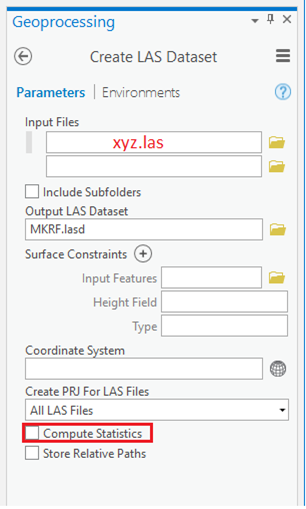
\includegraphics[width=0.4\linewidth]{images/04-creating-las-dataset} \end{center}

\hypertarget{q1.-what-is-the-correct-projection-for-this-dataset}{%
\paragraph*{Q1. What is the correct projection for this dataset?}\label{q1.-what-is-the-correct-projection-for-this-dataset}}
\addcontentsline{toc}{paragraph}{Q1. What is the correct projection for this dataset?}

\textbf{Step 2:} We can now add our LAS Dataset to a Map document (insert New Map). Depending on the zoom extent, you may only see the red bounding box of the las file; this isn't an error, you just need to zoom in to see the actual points. Alternatively, you can open the dataset in a `Global Scene', although due to the size of the point cloud this might cause some lag. The default display is that no point cloud filters are applied; if you want to view only ground points, right click on the file, navigate to `LAS Filters', and click `Ground'. If you want to investigate what the forest looks like, you can add the MKRF orthophoto.

\begin{center}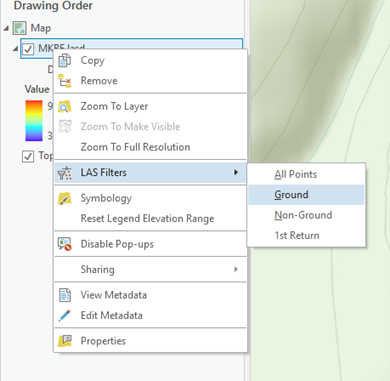
\includegraphics[width=0.4\linewidth]{images/04-view-and-filter-dataset} \end{center}

\hypertarget{q2.-what-is-the-average-point-spacing-of-the-dataset}{%
\paragraph*{Q2. What is the average point spacing of the dataset?}\label{q2.-what-is-the-average-point-spacing-of-the-dataset}}
\addcontentsline{toc}{paragraph}{Q2. What is the average point spacing of the dataset?}

\hypertarget{q3.-what-is-the-percentage-of-points-that-are-ground-points}{%
\paragraph*{Q3. What is the percentage of points that are ground points?}\label{q3.-what-is-the-percentage-of-points-that-are-ground-points}}
\addcontentsline{toc}{paragraph}{Q3. What is the percentage of points that are ground points?}

\begin{center}\rule{0.5\linewidth}{0.5pt}\end{center}

\hypertarget{task-2-create-a-dtm-using-built-in-arcgis-functions}{%
\section*{Task 2: Create a DTM using built-in ArcGIS functions}\label{task-2-create-a-dtm-using-built-in-arcgis-functions}}
\addcontentsline{toc}{section}{Task 2: Create a DTM using built-in ArcGIS functions}

\textbf{Step 1:} Now that we are familiar with the dataset, we can create a DTM using the easy to use built-in functions. To do so, search for the `LAS Dataset to Raster' tool, and use your LAS Dataset as the input. Since we are interested in creating a terrain model, we want to use the binning interpolation type, and make sure that we use the minimum (i.e.~the lowest) points in each cell assignment. Sampling Value refers to the resolution of the raster that we are creating -- we want our raster to be 30m x 30m. Name this raster \textbf{`MKRF\_DTM'}.

\begin{center}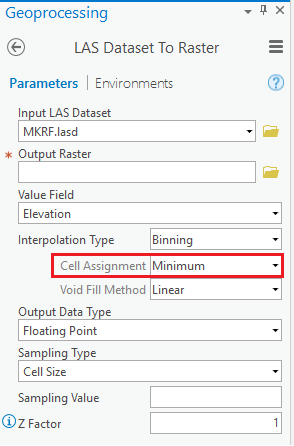
\includegraphics[width=0.4\linewidth]{images/04-las-dataset-to-raster} \end{center}

\hypertarget{q4.-why-is-it-important-to-select-the-minimum-value-in-the-cell-assignment-selection-2-sentence-maximum}{%
\paragraph*{Q4. Why is it important to select the minimum value in the cell assignment selection? (2 sentence maximum)}\label{q4.-why-is-it-important-to-select-the-minimum-value-in-the-cell-assignment-selection-2-sentence-maximum}}
\addcontentsline{toc}{paragraph}{Q4. Why is it important to select the minimum value in the cell assignment selection? (2 sentence maximum)}

Now that we have seen how to create a raster using the built-in functions, we can look at other methods and compare them to what we just created

\begin{center}\rule{0.5\linewidth}{0.5pt}\end{center}

\hypertarget{task-3-pre-process-data-for-interpolation}{%
\section*{Task 3: Pre-process data for interpolation}\label{task-3-pre-process-data-for-interpolation}}
\addcontentsline{toc}{section}{Task 3: Pre-process data for interpolation}

In order to access the raster interpolation toolset, we need to carry out some intermediate steps before we can treat the LAS Dataset as individual points.

\textbf{Step 1:} Extract LAS

This is where we extract only the ground points to be used for our interpolation. Make sure the \textbf{ground filter} is applied on our LAS Dataset, and then search for the `Extract LAS' tool. We can produce an output LAS Dataset to view on the Map, as well as a LAS file that we will use for the following steps. The result of this tool will be a new .las file with the suffix '\_ground'

We can test that this step has worked by looking at the properties in the catalog. We should have significantly fewer points in the ground dataset than the full dataset.

\begin{center}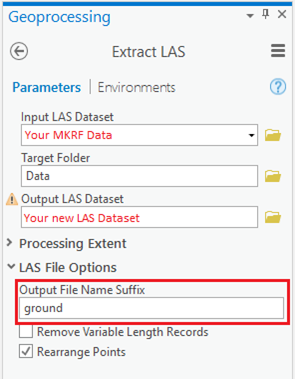
\includegraphics[width=0.4\linewidth]{images/04-extract-ground-points} \end{center}

\textbf{Step 2:} LAS to Multipoint

We need to convert our newly extracted LAS file to a multipoint feature class before we can use the multi to singlepart tool. In the `LAS to Multpoint' tool, input your new LAS file (the .las you created, not the .lasd). You will notice that there is a box asking for the `Average Point Spacing'. This is where we can use the LAS Dataset we created in the previous step to look up the statistics. Use this value, as well as the Coordinate System that we used previously, and run the tool.

\textbf{Step 3:} Multipart to Singlepart.

Search for the 'Multipart to Singlepart` tool, and use your multipoint feature class as the input. This might take a little while, so be patient!

\textbf{Step 4:} Add Z values

We can now add our height values to be used for interpolation. Search for the `Add Z Information' tool, and use your output from the `Multipart to Singlepart' process. The only output option available should be `Spot Z', make sure it is checked. We have now created a point feature class to test our interpolation on!

\begin{center}\rule{0.5\linewidth}{0.5pt}\end{center}

\hypertarget{task-4-raster-interpolation}{%
\section*{Task 4: Raster interpolation}\label{task-4-raster-interpolation}}
\addcontentsline{toc}{section}{Task 4: Raster interpolation}

If you haven't done so, now is a good time to save your project as creating these rasters can sometimes be tough on laptops. Since we now have points representing height values, we can use the raster interpolation toolset to experiment with 3 different interpolation techniques; Kriging, Inverse Distance Weighting (IDW), and Spline. To help understand more about these techniques, have a look at the online help section for the \href{https://pro.arcgis.com/en/pro-app/tool-reference/spatial-analyst/an-overview-of-the-interpolation-tools.htm}{interpolation toolset} (see each tool in the left hand menu):

\hypertarget{q5.-when-looking-at-semivariogram-properties-what-does-major-range-and-nugget-refer-to-two-sentence-maximum}{%
\paragraph*{Q5. When looking at semivariogram properties what does `major range' and `nugget' refer to? (two sentence maximum)}\label{q5.-when-looking-at-semivariogram-properties-what-does-major-range-and-nugget-refer-to-two-sentence-maximum}}
\addcontentsline{toc}{paragraph}{Q5. When looking at semivariogram properties what does `major range' and `nugget' refer to? (two sentence maximum)}

\textbf{Step 1:} Enter the name of each interpolation technique in the geoprocessing search window individually and explore their parameters. In order to make the comparison straightforward, make sure that the output raster is the same resolution as the DTM created in Task 2. Create 3 rasters: one using Spline, one using IDW, and one using Kriging. Note, when creating the rasters, keep the default settings, except for Kriging. For this tool, change the number of points in the search radius to 6. This will increase the speed of the tool, although it will still take a while!

\begin{center}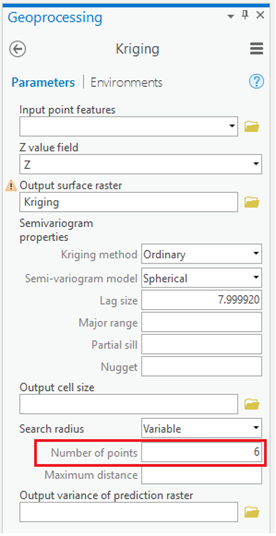
\includegraphics[width=0.4\linewidth]{images/04-dtm-using-kriging} \end{center}

\begin{center}\rule{0.5\linewidth}{0.5pt}\end{center}

\hypertarget{task-5-visually-interpret-differences}{%
\section*{Task 5: Visually interpret differences}\label{task-5-visually-interpret-differences}}
\addcontentsline{toc}{section}{Task 5: Visually interpret differences}

So far, we have created 4 rasters. Take some time to inspect each raster, and look at their similarities and differences (make sure that you are using a common symbology when comparing). If we consider the first raster that we created (MKRF\_DTM) as the `truth', we can compare the differences between our interpolated rasters in Task 4 with this DTM.

\textbf{Step 1:} In order to compare the rasters, we will make a raster of the differences between the interpolated surface and that of the `truth'. You will use the Raster Calculator tool to do this. We will calculate the absolute value of the difference of the two rasters. The statement in the Raster Calculator tool should look something like this:

\textbf{Abs(``MKRF\_DTM'' - ``IDW\_DTM'')}

Repeat this for all three interpolation methods (Spline, Kriging, and IDW), naming the results something like ``spline\_diff'', ``krig\_diff'', and ``idw\_diff''.

\hypertarget{q6.-which-interpolation-technique-most-closely-resembles-the-default-raster-mkrf_dtm-from-task-2}{%
\paragraph*{Q6. Which interpolation technique most closely resembles the default raster (MKRF\_DTM) from Task 2?}\label{q6.-which-interpolation-technique-most-closely-resembles-the-default-raster-mkrf_dtm-from-task-2}}
\addcontentsline{toc}{paragraph}{Q6. Which interpolation technique most closely resembles the default raster (MKRF\_DTM) from Task 2?}

\begin{center}\rule{0.5\linewidth}{0.5pt}\end{center}

\hypertarget{task-6-quantitatively-interpret-the-differences-and-calculate-statistics-for-each-zone}{%
\section*{Task 6: Quantitatively interpret the differences and calculate statistics for each zone}\label{task-6-quantitatively-interpret-the-differences-and-calculate-statistics-for-each-zone}}
\addcontentsline{toc}{section}{Task 6: Quantitatively interpret the differences and calculate statistics for each zone}

To do this, we will look at the differences in terms of the landscape. We will look to see if there are any patterns between areas of high, medium, and low elevation as well as areas of high, medium, and low slope.

\textbf{Step 1:}: First, you will need to reclassify the DTM into high, medium, and low areas. To do this, you will use the Reclassify tool. Use the MKRF\_DTM as the input and call the output elev\_cls. Use the following values for reclassification: 200-400, 400.00001-600, 600.00001-900.

\begin{center}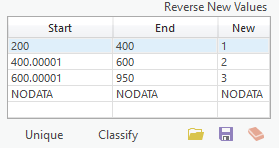
\includegraphics[width=0.4\linewidth]{images/04-reclassify-dtm} \end{center}

\textbf{Step 2:} Next, make and reclassify a slope feature class. Use the Slope tool to create a raster called mkrf\_slope from MKRF\_DTM. Next, use the Reclassify tool again to reclassify the mkrf\_slope and create a raster called slope\_cls using the following values: 0-15, 15.00001-30, 30.00001-90

\begin{center}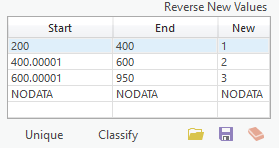
\includegraphics[width=0.4\linewidth]{images/04-reclassify-dtm} \end{center}

We will use these reclassified areas as zones to calculate statistics about the difference between the interpolated surface and the actual DTM. In both cases (slope\_cls and elev\_cls), higher values correspond to higher elevations and slopes.

\textbf{Step 3:} Calculate statistics for each zone

We will use Zonal Statistics to help us compare the differences between interpolation techniques. Search for `Zonal Statistics as Table' to have a cleaner output on our final map document.

We'll start with the elevations and IDW first. Open the Zonal Statistics as Table tool. The input raster or feature zone data is that which defines the zones. For us, this is elev\_cls, and the zone field is Value. The input value raster is going to be idw\_diff. Call the output table idw\_diff\_elev, and for Statistics type, only calculate the mean.

\begin{center}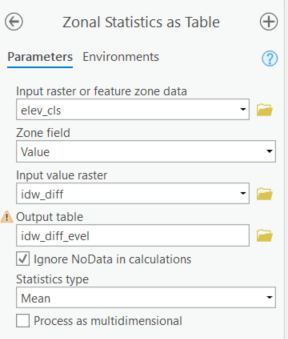
\includegraphics[width=0.4\linewidth]{images/04-zonal-statistics} \end{center}

Repeat this step for both topography classes (elevation and slope) as well as all three interpolation methods (IDW, Kriging, Spline). It can be useful to use the `History' button (in the Analysis tab), or ModelBuilder if you'd like.

In the end, you will make six tables called idw\_diff\_elev, idw\_diff\_slope, krig\_diff\_elev, krig \_diff\_slope, spline\_diff\_elev, and spline\_diff\_slope.

\begin{center}\rule{0.5\linewidth}{0.5pt}\end{center}

\hypertarget{task-7-create-a-map-document}{%
\section*{Task 7: Create a map document}\label{task-7-create-a-map-document}}
\addcontentsline{toc}{section}{Task 7: Create a map document}

\textbf{Step 1:} Switch ArcPro to layout view. You may change the page orientation to landscape instead of portrait if you'd like. To do so, go to File -\textgreater{} Page and Print Setup, and change the orientation to landscape.

\textbf{Step 2:} : In ArcGIS Pro, we can insert as many map frames as we want into our map layout. In our case, we will need 6 maps in our layout, as well as some free space for legends and text. There will be one interpolated surface and one difference raster for each of the three interpolation methods. Display each of these layers in their own map and place them appropriately in the layout. Each map should include only one raster, one of the following: DTMs using Spline, Kriging, and IDW, ``spline\_diff'', ``krig\_diff'', and ``idw\_diff''. Arrange the data frames by row and column so that the layout makes sense (that is, so each interpolation method is near one another.

\textbf{Step 3:} Add all of the tables from the previous step into one of the data frames. When you open these tables, you can add them to the map by clicking the Table Options selecting ``Add Table to Layout''. You can also remove unimportant columns from the display by right clicking the column name in the attribute table and clicking Turn Field Off. Place the tables in the layout view a way that makes sense (near their respective difference raster). Label what each of the values means with a text box (Insert -\textgreater{} Text).

\textbf{Step 4:} Change symbology for both the overall and difference layers. Use the same one for all of them.

Start with the elevations. Click on one of the layers representing the interpolated surfaces (Spline, for example) and select the the Symbology tab. Change the Primary symbology to `Classify'. Set the number of classes to 7. You may change the color ramp to one that makes sense to you, but make sure that there is enough contrast between classes. Change the symbology of the other two interpolated surfaces to match the first one (i.e.~make sure to match break classes). Hint: you can investigate the `Apply Symbology from Layer' tool to do this quickly.

Repeat the same process for the difference rasters. This time, use 8 classes and set the breaks so that they make sense (e.g.~2, 4, 6, 8, 10, 12, 14, and 50).

Add a legend for each symbology definition (Elevation and Difference) to the map layout by clicking on a data frame and selecting Insert -\textgreater{} Legend from the top menu bar. Place them on the map layout in a way that makes sense (near the respective layers).

Finally, put some text on the layout to communicate which data frame is which, and what each table represents. You can either label every data frame or label the columns and rows (``Interpolated Surface'' and ``Difference to DTM'' as rows and ``Spline'', ``Kriging'', and ``IDW'' as columns). Make sure you communicate what each aspect of the map is effectively!

Save the ArcMap document and export the map document to a PNG (Share -\textgreater{} Export Layout). When you're all done, it should look something like this:

\begin{center}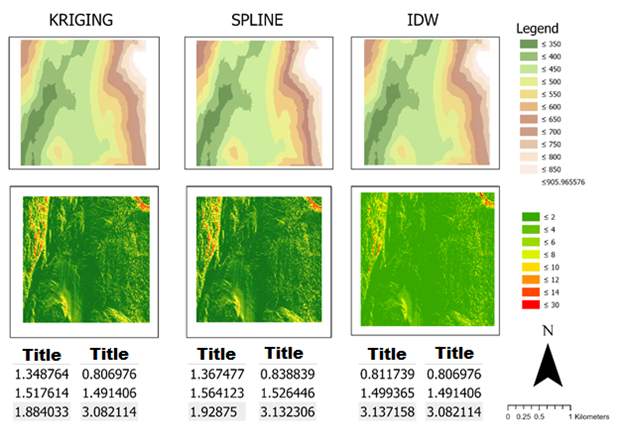
\includegraphics[width=0.75\linewidth]{images/04-map-document} \end{center}

\begin{center}\rule{0.5\linewidth}{0.5pt}\end{center}

\hypertarget{task-8-exploring-scenes}{%
\section*{Task 8: Exploring Scenes}\label{task-8-exploring-scenes}}
\addcontentsline{toc}{section}{Task 8: Exploring Scenes}

\textbf{Step 1:} The first thing that we will do is add a Local Scene (Insert New Map -\textgreater{} New Local Scene). Add the MKRF\_Aerial\_Photo to the scene. We can navigate through the scene using the mouse, or the \href{https://www.youtube.com/watch?v=vMLG3iduw50}{on-screen navigator}. You can learn more about navigation in Pro \href{https://pro.arcgis.com/en/pro-app/help/mapping/navigation/navigation-in-arcgis-pro.htm}{here}.

\begin{center}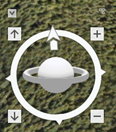
\includegraphics[width=0.15\linewidth]{images/04-on-screen-navigator} \end{center}

Take some time to play around and explore the scene. One thing we notice is that the imagery does not match the `ground'. This is because the ground in the scene is using the default global service, which has a resolution of between 10 and 30 meters. We need to create a custom ground surface to elevate the forest.

\textbf{Step 2:} In order for the data to more accurately reflect the real world, we can add a higher resolution digital surface model (DSM) to the area of interest. In Task 2, Step 1, we saw how to make a simple DTM using the LAS Dataset to Raster tool. We are now going to create a DSM to help us visualize our data in three dimensions. Using the same tool, create a raster called `MKRF\_DSM' with a resolution of 2 meters, binning the data by `Maximum'.

\textbf{Step 3:} In the Contents pane, right-click Ground, located below the Elevation Surfaces group layer. Click `Add Elevation Source'. Browse to the location of your newly created DSM and select it. You can now start to see how the surface features have been incorporated into the surface. Make sure to zoom in to look at areas with high relief and roads. Look at the cut block in the in the center of the scene. Why might these trees look strange?

\textbf{Step 4:} Sometimes it might be useful to exaggerate height differences to show a particular aspect of your dataset. To do this, click on `ground' and navigate to the `Appearance' tab (on the top bar). You can play around with the vertical exaggeration here and see how data is displayed differently. You might also be interested in changing the lighting of the scene in order to show what your data looks like at a certain time. Right click on `Scene' and select `Properties' (on the left side of the screen) to access illumination properties. This section is where you can experiment with the lighting of your scene (for example you can set a date and time).

\textbf{Step 5:} Export a scene of your choice. With a figure caption, describe what we are looking at, and whether you changed the vertical exaggeration or illumination in the scene.

\begin{center}\includegraphics[width=0.75\linewidth]{images/04-example-scene-MKRF} \end{center}

\hypertarget{summary-2}{%
\section*{Summary}\label{summary-2}}
\addcontentsline{toc}{section}{Summary}

In this lab, we explored the capabilities of ArcGIS to view, manipulate, and analyze LiDAR point cloud data. We harnessed the power and ease of use of the ArcGIS built-in functions for preprocessing the LiDAR and making a DTM. We tested three different interpolation methods when making our point cloud derived DTM: Kriging, Inverse Distance Weighting, and Spline. We looked for patterns based on low, medium, and high elevation and sloped areas across our different DTM products for more insight into how our choice of interpolation method will have an impact on our eventual data product. Moving then onto making a 3D scene in ArcGIS, we explored how to more accurately reflect the real world by ensuring the ground surface matches the forest. Finally, we ended on a discussion of highlighting particular characteristics of your dataset through changing the lighting or exagerating height differences within the ArcGIS scene.

Return to the \protect\hyperlink{lab4-deliverables}{\textbf{Deliverables}} section to check off everything you need to submit for credit in the course management system

\hypertarget{suitability-overlay-analysis}{%
\chapter{Suitability and Overlay Analysis}\label{suitability-overlay-analysis}}

Written by
Annie Mejaes

\hypertarget{lab-overview-3}{%
\section*{Lab Overview}\label{lab-overview-3}}
\addcontentsline{toc}{section}{Lab Overview}

Oftentimes, what we consider to be GIS analysis in the natural resources domain is related to suitability analysis. This analysis typically involves identifying areas/features that could support a given activity, use, or process and eliminating areas/features that would not be able to fulfill the required needs. Suitability analysis typically refers to an ordinal classification of the capable areas/features to denote the relative abilities of these areas/features to fulfill these needs. This number is mostly likely represented as an index that ranges from 0 to 1 where 1 = the most suitability possible for a given area/feature and 0 = no suitability. Typically, there will be no 0 values present in this index as all incapable areas should have already been eliminated in previous steps.

In order to perform a suitability analysis, geospatial operations, such as vector polygon overlay and database table intersection are not only the distinguishing functional characteristics of a geographic information system, but are also the most common aspects of this process. In order to gain an understanding of the potential of cartographic modeling using a GIS, this lab has been constructed to take you through an exercise that closely mirrors a prototypical GIS analysis related to conservation values.

Marine spatial planning is ``a collaborative and transparent approach to managing ocean spaces that helps to balance the increased demand for human activities with the need to protect marine ecosystems. It takes into consideration all activities and partners in an area to help make informed decisions about the management of our oceans in a more open and practical way.

Marine Spatial Planning is internationally recognized as an effective tool for transparent, inclusive and sustainable oceans planning and management. Approximately 65 countries are currently using this approach. Marine Spatial Plans are tailored to each unique area to help manage human activities and their impacts on our oceans. Depending on the area, these plans may include areas for potential resource development and areas that require special protection'' (Fisheries and Oceans Canada).

The State of Hawai'i defines Marine Protected Areas as ``a subset of MMAs, and focus on protection, enhancement, and conservation of habitat and ecosystems. Some MPAs have very few fishing restrictions and allow sustainable fishing, while others restrict all fishing and are ``no take'' areas. In Hawai`i, forms of MPAs have been in use for over 40 years.'' -Division of Aquatic Resources

Within this lab, we will utilize existing and new geospatial tools to conduct a marine spatial planning exercise in Hawaii, USA. You will complete tasks based on a scenario related to the critical habitat of cetaceans in Hawaii and conflicting uses. You will learn tools and processes while completing the first scenario that you can apply to complete the second scenario more independently.

\begin{enumerate}
\def\labelenumi{\arabic{enumi}.}
\item
  Considered one of the world's most important humpback whale habitats, the Hawaiian Islands Humpback Whale National Marine Sanctuary was established in 1992 to protect humpback whales (\emph{Megaptera novaeangliae}) and their habitat in Hawai`i. Humpback whales commonly give birth and raise their young in the state's warm and shallow waters. Yet, there is increasing conflict between the whales and vessels, including recreational and whale watching boats, as well as cargo ships. Thus, national and state government agencies would like to expand the marine sanctuary to reduce the whales strikes, further protecting the whales and their calves. The government agencies are searching for the largest suitable areas to include as part of the sanctuary.
\item
  False killer whales, an endangered resident species in Hawaiian waters, are long-lived and only reproduce one calf every 6 or 7 years. So, the species is heavily impacted by human activities, taking a long time to recover. The false killer whales are often caught in fishing gear as bycatch, which is defined as the incidental or unintentional capture of a non-target species. Not only is this severely hurting the false killer whale population, in addition, Hawaiian fisheries have been forced to close their fishing season early, by reaching their bycatch limit. As there is a resource conflict at play, you will need to redefine the fishing grounds to limit the bycatch, as well as discuss the placement of a marine sanctuary for false killer whales.
\end{enumerate}

\begin{center}\rule{0.5\linewidth}{0.5pt}\end{center}

\hypertarget{learning-objectives-4}{%
\section*{Learning Objectives}\label{learning-objectives-4}}
\addcontentsline{toc}{section}{Learning Objectives}

\begin{itemize}
\tightlist
\item
  Practice good data management principles
\item
  Distinguish overlay tools and recognize when to apply them
\item
  Calculate a weighted suitability index
\item
  Identify and map the most suitable locations for new marine sanctuaries
\end{itemize}

\begin{center}\rule{0.5\linewidth}{0.5pt}\end{center}

\hypertarget{lab5-deliverables}{%
\section*{Deliverables}\label{lab5-deliverables}}
\addcontentsline{toc}{section}{Deliverables}

Scenario 1:

\begin{itemize}
\tightlist
\item
  An output table of the top 5 ranked features (see Task 7)
\item
  Map of the final product
\item
  a screenshot of the geodatabase
\item
  a \href{https://www.usgs.gov/data-management/data-dictionaries}{data dictionary} - includes all files in the gdb
\item
  answers to the questions submitted to the Lab 4 section on Canvas
\end{itemize}

Scenario 2:

\begin{itemize}
\tightlist
\item
  Two page report including your findings, which should also include at least one table and two maps in the appendix (not counting toward the page count)
\end{itemize}

Report should satisfy the following requirements:

\begin{itemize}
\tightlist
\item
  place maps and tables at the end of the document
\item
  1'' margins
\item
  12 point font
\item
  single spaced
\item
  maximum of two pages
\item
  structure as a technical report where you are given a recommendation to someone, trying to make a case as to why this should happen
\item
  use headings as needed
\item
  omit your name, student number, date
\end{itemize}

In addition to including relevant maps, please answer the following questions in your report:

\begin{itemize}
\tightlist
\item
  What did you learn from Scenario 2 Tasks 3 and 4?
\item
  How would you conduct a suitability analysis to determine the location of a marine sanctuary for false killer whales? What other factors could you consider?
\item
  Why is it important to consider multiple dimensions in a suitability analysis?
\end{itemize}

\begin{center}\rule{0.5\linewidth}{0.5pt}\end{center}

\hypertarget{data-3}{%
\section*{Data}\label{data-3}}
\addcontentsline{toc}{section}{Data}

The relevant data is located in your Canvas folder. You will be expected to practice proper data management by updating the existing file geodatabase with new shapefiles that are produced. Utilize what you have learnt in the past labs regarding the geodatabase creation, including using best practices regarding naming conventions.

\hypertarget{data-organization}{%
\subsection*{Data Organization}\label{data-organization}}
\addcontentsline{toc}{subsection}{Data Organization}

You will find this lab much easier if you keep your data in a structure that makes sense for you -- and others (as much as possible!) -- by using meaningful names. As you progress through each step, we recommend that you also take a look at your data and use tools to delete unnecessary fields in your attribute tables so that they are not overpopulated and confusing.

\hypertarget{files-to-create}{%
\subsection*{Files to Create}\label{files-to-create}}
\addcontentsline{toc}{subsection}{Files to Create}

Here is a table of files you will be creating:

\begin{tabular}{ll}
\toprule
File Name & Created in Task\\
\midrule
Humpback\_BIA & 1\\
Humpback\_Hawaii\_BIA & 1\\
BIA\_Sanctuary\_Erase & 2\\
BIA\_Sightings & 3\\
BIA\_Multipart & 3\\
\addlinespace
BIA\_Sightings\_Multipart & 3\\
Boat\_Uses & 4\\
BIA\_Sightings\_Boat & 5\\
Top\_Five\_Sanctuary & 7\\
Sanctuary\_Buffer & 7\\
\bottomrule
\end{tabular}

\begin{center}\rule{0.5\linewidth}{0.5pt}\end{center}

\hypertarget{scenario-1}{%
\section*{Scenario 1}\label{scenario-1}}
\addcontentsline{toc}{section}{Scenario 1}

\hypertarget{task-1-export-relevant-data-from-biologically-important-areas-shapefile}{%
\section*{Task 1: Export Relevant Data from Biologically Important Areas Shapefile}\label{task-1-export-relevant-data-from-biologically-important-areas-shapefile}}
\addcontentsline{toc}{section}{Task 1: Export Relevant Data from Biologically Important Areas Shapefile}

A biologically important area (BIA) identifies where cetaceans concentrate for specific behaviours. Download the Lab 7 data from your Canvas folder and connect the geodatabase to your new Map. Explore the file \textbf{Cetaceans\_BIA}.

You will need to extract the BIA for the humpback whales from the other species.

\textbf{Step 1:} Start a new project in ArcGIS Pro.

\textbf{Step 2:} Connect to the \texttt{whale} database on the UBC PostgreSQL server in ArcGIS Pro. Add \textbf{Cetaceans\_BIA} to your map in ArcGIS Pro.

\textbf{Step 3:} Right-click on the layer and select `Attribute Table'. Explore the attribute table and understand what field you will need to use to extract `Humpback Whale'.

\textbf{Step 4:} Right-click on the layer again, select `Data', and then select `Export Features'. Write a SQL query to extract the BIA for the humpback whales from the other species and save the output to your local geodatabase in your ArcGIS Pro project. Ensure the file is added to your map in ArcGIS Pro and then explore the new layer and attribute table.

\hypertarget{q1.-what-was-the-sql-expression-that-you-used-to-export-only-the-humpback-whale-bia}{%
\paragraph*{Q1. What was the SQL expression that you used to export only the humpback whale BIA?}\label{q1.-what-was-the-sql-expression-that-you-used-to-export-only-the-humpback-whale-bia}}
\addcontentsline{toc}{paragraph}{Q1. What was the SQL expression that you used to export only the humpback whale BIA?}

\hypertarget{q2.-apart-from-hawaii-does-the-humpback-whale-have-any-other-locations-with-a-bia-for-reproduction-1-point}{%
\paragraph*{Q2. Apart from Hawaii, does the humpback whale have any other locations with a BIA for reproduction? (1 point)}\label{q2.-apart-from-hawaii-does-the-humpback-whale-have-any-other-locations-with-a-bia-for-reproduction-1-point}}
\addcontentsline{toc}{paragraph}{Q2. Apart from Hawaii, does the humpback whale have any other locations with a BIA for reproduction? (1 point)}

\textbf{Step 5:} Repeat Step 4, but this time only export the humpback whale BIA for Hawaii and name the file \textbf{Humpback\_Hawaii\_BIA}.

\begin{center}\rule{0.5\linewidth}{0.5pt}\end{center}

\hypertarget{task-2-identify-the-bia-of-the-humpback-whale-that-is-not-within-the-established-marine-sanctuary}{%
\section*{Task 2: Identify the BIA of the Humpback Whale that is not within the established Marine Sanctuary}\label{task-2-identify-the-bia-of-the-humpback-whale-that-is-not-within-the-established-marine-sanctuary}}
\addcontentsline{toc}{section}{Task 2: Identify the BIA of the Humpback Whale that is not within the established Marine Sanctuary}

Visually compare the Marine Sanctuary (\textbf{Humpback\_Marine\_Sanctuary}) to the BIA of the humpback whale population.

\textbf{Step 1:} Open the tool `Overlay Layers'.

\textbf{Step 2:} Within the tool, the input layer should be the BIA, the overlay layer is the sanctuary. For `Overlay Type', select Erase. Name the output \textbf{BIA\_Sanctuary\_Erase}.

\includegraphics[width=0.5\linewidth]{images/05-overlay-layers}

\hypertarget{q3.-what-percentage-of-the-bia-is-outside-of-the-marine-sancuary-hint-use-the-attribute-tables.}{%
\paragraph*{Q3. What percentage of the BIA is outside of the marine sancuary? Hint: Use the attribute tables.}\label{q3.-what-percentage-of-the-bia-is-outside-of-the-marine-sancuary-hint-use-the-attribute-tables.}}
\addcontentsline{toc}{paragraph}{Q3. What percentage of the BIA is outside of the marine sancuary? Hint: Use the attribute tables.}

\includegraphics[width=0.75\linewidth]{images/05-bia-sanctuary-erase-attribute-table}

\begin{center}\rule{0.5\linewidth}{0.5pt}\end{center}

\hypertarget{task-3-calculate-the-density-of-cetacean-sightings-using-the-bia-for-humpback-whales}{%
\section*{Task 3: Calculate the Density of Cetacean Sightings using the BIA for Humpback Whales}\label{task-3-calculate-the-density-of-cetacean-sightings-using-the-bia-for-humpback-whales}}
\addcontentsline{toc}{section}{Task 3: Calculate the Density of Cetacean Sightings using the BIA for Humpback Whales}

Next, we have a point layer named \textbf{Humpback\_Sightings} that is curated based on where cetaceans have been located or identified in Hawaiian waters. We want to understand the density of the sightings within the remaining BIA layer to understand which polygons should be prioritized.

\textbf{Step 1:} Open the tool `Spatial Join'. Spatial Join is a valuable tool that joins attributes from one feature to another based on a spatial relationship. The target feature defines the spatial boundary, while the input feature is molded to the target feature.

\textbf{Step 2:} Within the tool, the target features are \textbf{BIA\_Sanctuary\_Erase}, the input feature is \textbf{Humpback\_Sightings}, and the join operation is `Join one to one'. The match option is `Contains'. Name the output \textbf{BIA\_Sightings}.

\includegraphics[width=0.5\linewidth]{images/05-spatial-join}

\textbf{Step 3:} Open the attribute table. What do you see went wrong with this analysis?

We need to introduce a new tool, `Multipart to Singlepart' to fix this problem. After you have used the `Overlay Layers' to erase features from the BIA for humpback whales, you will be left with several polygons that are still considered the same polygon by ArcGIS Pro, but are now spatially separated (refer to the help page for \href{https://pro.arcgis.com/en/pro-app/latest/tool-reference/data-management/multipart-to-singlepart.htm}{Multipart to Singlepart tool}). Try finding one and selecting it. You will know it is multipart when a number of additional polygons are outlined when you click one polygon. You will need to separate those parts into unique polygons before continuing on to the next step. What this is allowing you to do is to recommend placement of the expanded marine sanctuary into a portion of a BIA.

\textbf{Step 4:} Open the `Multipart to Singlepart' tool and select the input layer as the layer \textbf{BIA\_Sanctuary\_Erase}.

\hypertarget{q4.-how-many-individual-polygons-now-exist}{%
\paragraph*{Q4. How many individual polygons now exist?}\label{q4.-how-many-individual-polygons-now-exist}}
\addcontentsline{toc}{paragraph}{Q4. How many individual polygons now exist?}

\textbf{Step 5}: Now re-do `Spatial Join' from Steps 1-2. There are many polygons that have a minimal area, so, unselect `Keep all Target Features', which will remove polygons that do not have any cetacean sightings within its boundaries.

\textbf{Step 6:} Use symbology to display the BIA polygons by number of cetacean sightings.

\includegraphics[width=0.75\linewidth]{images/05-bia-polygons}

\hypertarget{q5.-what-is-the-target_fid-of-the-polygon-with-the-most-cetacean-sightings}{%
\paragraph*{Q5. What is the Target\_FID of the polygon with the most cetacean sightings?}\label{q5.-what-is-the-target_fid-of-the-polygon-with-the-most-cetacean-sightings}}
\addcontentsline{toc}{paragraph}{Q5. What is the Target\_FID of the polygon with the most cetacean sightings?}

\begin{center}\rule{0.5\linewidth}{0.5pt}\end{center}

\hypertarget{task-4-extract-the-boats-from-ocean-uses-and-identity-the-vessels-within-the-bia-polygons}{%
\section*{Task 4: Extract the Boats from Ocean Uses and Identity the Vessels within the BIA Polygons}\label{task-4-extract-the-boats-from-ocean-uses-and-identity-the-vessels-within-the-bia-polygons}}
\addcontentsline{toc}{section}{Task 4: Extract the Boats from Ocean Uses and Identity the Vessels within the BIA Polygons}

The \textbf{Ocean\_Uses} layer contains a wide range of human activities that occur at the coast or in the ocean. We would like to extract `Motorized Boating', `Wildlife Viewing at Sea', `Commercial Pelagic Fishing', `Cruise Ships', and `Shipping'. These human activities pose the most threat to humpback whales, and, so, we would like to expand the sanctuary to protect humpback whales where their current risk of collision with a vessel is the highest.

\textbf{Step 1:} Export features where Motorized Boating or any of the other human activities mentioned above is equal to `Dominant Use' (value of 2). Be sure to set the output location to your local ArcGIS Pro project geodatabase and name the output feature class \textbf{Boat\_Uses}.

\includegraphics[width=0.5\linewidth]{images/05-feature-class-to-feature-class}

Now, we would like to bring the data on vessel usage and the BIA polygons together using the Overlay Layers tool. This is important to be able to see the spatial overlap between where humpback whales reproduce and rear their young and where vessels are labeled as a Dominant Use, indicating that there is a higher chance of boat strikes in these locations.

\textbf{Step 2:} Open the tool `Overlay Layers'. The input layer should be \textbf{BIA\_Sightings\_Multipart} and the overlay layer is \textbf{Boat\_Uses}. For `Overlay Type', select Identity. Name the output \textbf{BIA\_Sightings\_Boat}.

\hypertarget{q6.-open-the-attribute-table-for-the-output.-what-does-the-0-1-and-2-represent-in-the-swimming-column}{%
\paragraph*{Q6. Open the attribute table for the output. What does the 0, 1, and 2 represent in the swimming column?}\label{q6.-open-the-attribute-table-for-the-output.-what-does-the-0-1-and-2-represent-in-the-swimming-column}}
\addcontentsline{toc}{paragraph}{Q6. Open the attribute table for the output. What does the 0, 1, and 2 represent in the swimming column?}

\begin{center}\rule{0.5\linewidth}{0.5pt}\end{center}

\hypertarget{task-5-calculate-suitability-and-identify-most-suitable-locations-for-the-marine-sanctuary}{%
\section*{Task 5: Calculate Suitability and Identify Most Suitable Locations for the Marine Sanctuary}\label{task-5-calculate-suitability-and-identify-most-suitable-locations-for-the-marine-sanctuary}}
\addcontentsline{toc}{section}{Task 5: Calculate Suitability and Identify Most Suitable Locations for the Marine Sanctuary}

Now, we will determine where is the most suitable location to expand the marine sanctuary for humpback whales. The suitability value will be a new field between the value of 0 and 1 with 1 being the most suitable, and 0 being not suitable. It will be based on 3 characteristics (suitability factors):

\begin{itemize}
\tightlist
\item
  the larger the area the higher the suitability score
\item
  the more cetacean sightings per area, within an area the higher the suitability score
\item
  the more dominant ocean uses the higher the suitability score
\end{itemize}

\textbf{Step 1:} Before you calculate final suitability score, you will need to add three new fields to \textbf{BIA\_Sightings\_Boat} within the attribute table:

\begin{itemize}
\tightlist
\item
  Area (float)
\item
  Sightings (float)
\item
  Vessels (float)
\end{itemize}

\textbf{Step 2:} For each of the three fields you just added, you will need to calculate \([F /Fmax]\) for each record (row):

\begin{itemize}
\tightlist
\item
  \(F\) is the value of the attribute for that record
\item
  \(Fmax\) is the maximum record value for the field
\end{itemize}

\emph{HINT: Always add a decimal point to the Fmax so that the result is a floating point decimal number.}

First, determine \(Fmax\) for Area (use Shape Area field for \(Fmax\)), Sightings (use Join Count), and Vessels (calculate manually based on the number of columns). Then, Right-click on the field in the attribute table and view statistics (write down the number that appears beside `maximum'). Finally, right-click on the field and select `Calculate Field' and enter the expression using the correct field name and the maximum value for the field.

\includegraphics[width=0.5\linewidth]{images/05-calculate-field}

\emph{HINT: For Vessels, you will need to include more than one column for \(F\).}

\textbf{Step 3:} Finally, use a weighted suitability calculation by creating a new field, Suitability, and writing the following expression:
{[}Area{]} * 0.4 + {[}Sightings{]} * 0.2 + {[}Vessels{]} * 0.4.

\hypertarget{q7.-write-down-the-fmax-value-you-used-for-area-to-four-decimal-places.}{%
\paragraph*{\texorpdfstring{Q7. Write down the \(Fmax\) value you used for area to four decimal places.}{Q7. Write down the Fmax value you used for area to four decimal places.}}\label{q7.-write-down-the-fmax-value-you-used-for-area-to-four-decimal-places.}}
\addcontentsline{toc}{paragraph}{Q7. Write down the \(Fmax\) value you used for area to four decimal places.}

\hypertarget{q8-write-down-the-fmax-value-you-used-for-sightings-to-four-decimal-places.}{%
\paragraph*{\texorpdfstring{Q8: Write down the \(Fmax\) value you used for sightings to four decimal places.}{Q8: Write down the Fmax value you used for sightings to four decimal places.}}\label{q8-write-down-the-fmax-value-you-used-for-sightings-to-four-decimal-places.}}
\addcontentsline{toc}{paragraph}{Q8: Write down the \(Fmax\) value you used for sightings to four decimal places.}

\hypertarget{q9-write-down-the-fmax-value-you-used-for-vessels-to-four-decimal-places}{%
\paragraph*{\texorpdfstring{Q9: Write down the \(Fmax\) value you used for vessels to four decimal places}{Q9: Write down the Fmax value you used for vessels to four decimal places}}\label{q9-write-down-the-fmax-value-you-used-for-vessels-to-four-decimal-places}}
\addcontentsline{toc}{paragraph}{Q9: Write down the \(Fmax\) value you used for vessels to four decimal places}

To provide a buffer zone protecting the humpback whales within the newly formed sanctuary, we will select the five BIA areas with the highest suitability score and create a five kilometer buffer.

\textbf{Step 4:} Sort the Suitability field by right-clicking on the field title and selecting \textbf{Sort Descending}.

\textbf{Step 5:} Select and export the top five features to a new layer named \textbf{Top\_Five\_Sanctuary}. Clean up the attribute table, so that it only has relevant columns. \textbf{This is the output table that is a deliverable for the lab.}

\textbf{Step 6:} Open the tool \textbf{Buffer}. Input features will be \textbf{Top\_Five\_Sanctuary}. Name the output \textbf{Sanctuary\_Buffer}. Set the distance as 5 kilometers. For dissolve type, select \textbf{Dissolve all output features into a single feature}.

You just conducted a suitability analysis and produced a map of how to potentially expand the humpback whale sanctuary!

Now is the time for your cartographic skills to shine. To design a map of the highest quality you will need to draw on all of you GIS skills. Ensure you include all the standard components of a map along with your artistic flair.

Also, be sure to include important data, but also make sure the map is not too cluttered. Remember that you can use inset maps to demonstrate additional detail for the most suitable habits.

The physical requirements are as follows:

\begin{itemize}
\tightlist
\item
  Map should be 11''x17'' either as a landscape or portrait layout
\item
  You should export the map as a PDF document
\item
  All features on the map should appear in the legend
\item
  Your map should have all the necessary elements of a map
\end{itemize}

\begin{center}\rule{0.5\linewidth}{0.5pt}\end{center}

\hypertarget{scenario-2}{%
\section*{Scenario 2}\label{scenario-2}}
\addcontentsline{toc}{section}{Scenario 2}

False killer whales, an endangered resident species in Hawaiian waters, are long-lived and only reproduce one calf every 6 or 7 years. So, the species is heavily impacted by human activities, taking a long time to recover. The false killer whales are often caught in fishing gear as bycatch, which is defined as the incidental or unintentional capture of a non-target species. Not only is this severely hurting the false killer whale population, in addition, Hawaiian fisheries have been forced to close their fishing season early, by reaching their bycatch limit. As there is a resource conflict at play, you will need to redefine the fishing grounds to limit the bycatch, as well as discuss the placement of a marine sanctuary for false killer whales.

Using the tools that you learned in Scenario 1. Please complete the below tasks.

\begin{center}\rule{0.5\linewidth}{0.5pt}\end{center}

\hypertarget{task-1-export-relevant-data-from-biologically-important-areas-shapefile-1}{%
\section*{Task 1: Export Relevant Data from Biologically Important Areas Shapefile}\label{task-1-export-relevant-data-from-biologically-important-areas-shapefile-1}}
\addcontentsline{toc}{section}{Task 1: Export Relevant Data from Biologically Important Areas Shapefile}

From this task, you will be able to identify where is the BIA for false killer whales in Hawaii. Try to only use one SQL expression to extract the data for species and region.

\begin{center}\rule{0.5\linewidth}{0.5pt}\end{center}

\hypertarget{task-2-extract-all-of-the-commercial-fishing-vessels-from-ocean-uses}{%
\section*{Task 2: Extract All of the Commercial Fishing Vessels from Ocean Uses}\label{task-2-extract-all-of-the-commercial-fishing-vessels-from-ocean-uses}}
\addcontentsline{toc}{section}{Task 2: Extract All of the Commercial Fishing Vessels from Ocean Uses}

From this task, you will obtain a shapefile of the relevant fishing vessels that are in conflict with the false killer whales. The fishing vessel types include: Commercial Fishing with Benthic Fixed Gear, Commercial Fishing with Benthic Mobile Gear, and Commercial Pelagic Fishing. Hint: Export Data for Dominant Uses of the above fields.

\begin{center}\rule{0.5\linewidth}{0.5pt}\end{center}

\hypertarget{task-3-erase-where-the-false-killer-whales-and-commercial-fishing-vessels-overlap}{%
\section*{Task 3: Erase where the False Killer Whales and Commercial Fishing Vessels overlap}\label{task-3-erase-where-the-false-killer-whales-and-commercial-fishing-vessels-overlap}}
\addcontentsline{toc}{section}{Task 3: Erase where the False Killer Whales and Commercial Fishing Vessels overlap}

Use the Overlay Layers tool to determine where the BIA for false killer whales in not in conflict with the fishing vessels. You can also determine where there is the most conflict between false killer whales and fishing vessels by using the `Identity' feature of the Overlay Layers tool, and then carrying out a calculation within the attribute table.

Explore the Number of other Species with BIAs that may also Conflict with the Commercial Fishing Vessels How does this impact how a marine sanctuary for false killer whales should be identified?

\begin{center}\rule{0.5\linewidth}{0.5pt}\end{center}

\hypertarget{summary-3}{%
\section*{Summary}\label{summary-3}}
\addcontentsline{toc}{section}{Summary}

Suitability modeling is a very common type of analysis that usually integrates multiple factors as geospatial layers using overlay and proximity tools. As you can imagine, there are many ways to structure this analysis and different weightings in the suitability calculation will yield entirely different results. Therefore, it is always important to maintain good justification and rationale for the weightings that you choose and any limitations in the analysis (e.g., missing data/information, incomplete or unavailable attributes, etc.) are clearly communicated in any recommendations that you make from your analysis. In this lab, you were also exposed to significant data manipulation and management. Using good data organization and naming conventions helps others understand your analysis and output data, including your future self if you ever need to return to your old work.

Return to the \textbf{\protect\hyperlink{lab5-deliverables}{Deliverables}} section to check off everything you need to submit for credit in the course management system.

\hypertarget{geographically-weighted-regression}{%
\chapter{Analyzing Green Equity Using Geographically Weighted Regression}\label{geographically-weighted-regression}}

Written by
Paul Pickell

\hypertarget{lab-overview-4}{%
\section*{Lab Overview}\label{lab-overview-4}}
\addcontentsline{toc}{section}{Lab Overview}

In this lab, you will be exploring a few different statistical approaches to modelling geographic data, including geographically weighted regression (GWR). GWR is the spatial extension of aspatial regression analysis and much more. Traditional regression analysis assumes that global statistics adequately describe local relationships that might exist in the data. For example, consider looking at the relationship between housing prices and the floor space, lot size, etc., of houses in the city of Vancouver. While we could develop a `global' model that adequately describes the relationship between those variables, knowing what you do about housing prices in the city of Vancouver (e.g., that a house of similar dimensions, age, lot size, etc., in the east side of Vancouver will sell for hundreds of thousands of dollars less than an identical house in the west side of Vancouver), the utility of such a model when looking at neighborhood-level housing issues would be very doubtful. Nonetheless, for decades such models, such as hedonic models, have been normalized in real estate research.

Similarly, consider studying the relationship between rates of crime or diseases to environmental conditions, local conditions can be much more important than any global relationship that might be discovered via a traditional aspatial statistical approach. Using polygon or point data, GWR allows us to explore the local relationships amongst a set of variables and examine the results spatially using ArcGIS Pro. It should be noted that in R you can find more sophisticated approaches to GWR than what is provided by ArcGIS Pro.

In this lab, you will explore the equity of green space for the city of Vancouver using Landsat imagery and demographic data from the 2021 Canadian census.

Why is access to green spaces so important? Human well-being, including physical and psychological well-being increase when residents are exposed to green space and urban forests. In addition, ecosystem services provided from green spaces include improved air quality, urban heat island mitigation, and opportunities for recreation. Yet, there is unequal access to green spaces across urban landscapes. The distribution of green space is often disproportionately present in affluent communities. So, you will test the hypothesis that there is less green space in marginalized communities. We cannot infer any causal relationships, but we can examine the relationship between the location of green spaces and demographic variables.

Vancouver is the most populous city in British Columbia, Canada with a population of 662,248 in 2021. Vancouver is an ideal study site because of the city's high level of heterogeneity among its demographic and green space structure.

\begin{center}\rule{0.5\linewidth}{0.5pt}\end{center}

\hypertarget{learning-objectives-5}{%
\section*{Learning Objectives}\label{learning-objectives-5}}
\addcontentsline{toc}{section}{Learning Objectives}

\begin{itemize}
\item
  Apply advanced SQL and PostGIS functions to a relational database to prepare high-dimensional census data for analysis
\item
  Calculate a vegetation index from Landsat imagery and report summary statistics over census dissemination areas
\item
  Evaluate different models and defend your model selection
\item
  Interpret charts and statistics of ordinary least squares and geographically weighted regression
\item
  Map geographically weighted regression results and interpret and defend your conclusions
\end{itemize}

\begin{center}\rule{0.5\linewidth}{0.5pt}\end{center}

\hypertarget{lab6-deliverables}{%
\section*{Deliverables}\label{lab6-deliverables}}
\addcontentsline{toc}{section}{Deliverables}

Lab report with the following specification:

6 pages maximum PDF including figures, tables and references (3 points). Single-spaced, 12-point Times New Roman font (1 point). All

Results should address the following questions and requirements (25 points):

\begin{itemize}
\item
  Describe the qualities of the census data and the Landsat image.
\item
  How did you evaluate your models and select your final model? Report any relevant statistics that you used in your judgement.
\item
  A table with the ordinary least squares and geographically weighted regression results for the models that used the best subsets of your 14 characteristics.
\item
  Describe all of the terms, coefficients, and explanatory variables of your selected GWR model.
\item
  Justify your choice of a final set of independent variables for your GWR model.
\item
  Compare and contrast the different NDVI statistics. Which statistic had the best model? What evidence do you have for that conclusion? Why do you think that relationship was the strongest?
\item
  Interpret one of your independent variables in one of your three NDVI statistics using the Std.Error and Coefficient map. What spatial patterns do you see? What do you think could be influencing this relationship?
\item
  Maps illustrating the standardized residuals and local R\^{}\{2\} for each of your three different NDVI statistics.
\end{itemize}

Discussion should address the following questions and requirements (20 points):

\begin{itemize}
\item
  What other factors (spatial or aspatial) might be contributing or confounding your analysis? In other words, what other data sources might you add/calculate or what methods might you change to improve your results?
\item
  What can you conclude about green equity among dissemnination areas in Vancouver?
\item
  What are your final recommendations to city council about green equity in Vancouver?
\item
  Reference to any peer reviewed sources as needed.
\end{itemize}

\begin{center}\rule{0.5\linewidth}{0.5pt}\end{center}

\hypertarget{lab6-data}{%
\section*{Data}\label{lab6-data}}
\addcontentsline{toc}{section}{Data}

All data for this lab are accessible from the course management system. The data provided on the course management system are a subset of the following public datasets:

Statistics Canada. 2022. Census Profile. 2021 Census. Statistics Canada Catalogue no. 98-316-X2021001. Ottawa. Released December 15, 2022. \url{https://www12.statcan.gc.ca/census-recensement/2021/dp-pd/prof/index.cfm?Lang=E}

We are using only a small subset of the national 2021 census data set for British Columbia: ``Canada, provinces, territories, census divisions (CDs), census subdivisions (CSDs) and dissemination areas (DAs) - British Columbia only'' (Statistics Canada Catalogue no. 98-401-X2021006).

The Statistics Canada 2021 spatial boundary files are maintained separately and available for download from here: \url{https://www12.statcan.gc.ca/census-recensement/2021/geo/sip-pis/boundary-limites/index2021-eng.cfm?year=21}

The spatial data from Statistics Canada that we will be using:

\begin{longtable}[]{@{}ll@{}}
\toprule\noalign{}
Layer Name & Description \\
\midrule\noalign{}
\endhead
\bottomrule\noalign{}
\endlastfoot
lcsd000b21a\_e & Census subdivisions \\
lda\_000b21a\_e & Dissemination areas \\
\end{longtable}

If you are a student at UBC, these data have already been prepared and loaded into the course management system. The links above are only for reference.

Metadata for the 2021 spatial boundary files can be found here: \url{https://www150.statcan.gc.ca/n1/pub/92-160-g/92-160-g2021002-eng.htm}

The Dictionary for Census of Population 2021 can be found here: \url{https://www12.statcan.gc.ca/census-recensement/2021/ref/dict/index-eng.cfm}

\begin{center}\rule{0.5\linewidth}{0.5pt}\end{center}

\hypertarget{task-1-visualize-census-data}{%
\section*{Task 1: Visualize census data}\label{task-1-visualize-census-data}}
\addcontentsline{toc}{section}{Task 1: Visualize census data}

Statistics Canada census data are distributed in tables. These data can be particularly challenging to work with because they span multiple geographical hierarchies (e.g., national, provincial, municipal, etc.), multiple dates (the Canadian census occurs every 5 years), many demographic dimensions (e.g., population, age, education, language, etc.), and there are an enormous amount of enumerated areas.

The smallest geographic unit that census data are enumerated over are known as Dissemination Areas (DA). Statistics Canada gives the definition:

\begin{quote}
A dissemination area (DA) is a small, relatively stable geographic unit composed of one or more adjacent dissemination blocks with an average population of 400 to 700 persons based on data from the previous Census of Population Program. It is the smallest standard geographic area for which all census data are disseminated. DAs cover all the territory of Canada.
\end{quote}

As of the 2021 Canadian census, there are 57,936 unique Dissemination Areas. Each Dissemination Area is described by 2,631 unique characteristics (total population, age, education, language, etc.). That is a whopping 152 million values for describing Canadians! Lucky for us, we will be working with DAs for Vancouver, British Columbia and only a handful of characteristics.

The census data that you have been provided with for this lab, available from the course management system, are the result of collating the values of some select characteristics from this massive census database for just the dissemination areas that cover the city of Vancouver. The characteristics are summarized in the table below:

\begin{longtable}[]{@{}
  >{\raggedright\arraybackslash}p{(\columnwidth - 4\tabcolsep) * \real{0.3455}}
  >{\raggedright\arraybackslash}p{(\columnwidth - 4\tabcolsep) * \real{0.3273}}
  >{\raggedright\arraybackslash}p{(\columnwidth - 4\tabcolsep) * \real{0.3273}}@{}}
\toprule\noalign{}
\begin{minipage}[b]{\linewidth}\raggedright
Characteristic
\end{minipage} & \begin{minipage}[b]{\linewidth}\raggedright
Units
\end{minipage} & \begin{minipage}[b]{\linewidth}\raggedright
Name
\end{minipage} \\
\midrule\noalign{}
\endhead
\bottomrule\noalign{}
\endlastfoot
Population, 2021 & Persons & population \\
Population density per square kilometre & Persons per square kilometre & popdensity \\
Total - Private households by household size - 100\% data & Families & households \\
Average household size & Persons & hhsize \\
Prevalence of low income based on the Low-income measure, after tax (LIM-AT) (\%) & \% & lowincome \\
Bachelor's degree or higher & Persons & education \\
Average age of the population & Years & age \\
0 to 14 years & \% & children \\
65 years and over & \% & seniors \\
Unemployment rate & \% & unemployment \\
Median total income in 2020 among recipients (\$) & \$ & medianincome \\
First official language spoken is neither English nor French & Persons & neitherenglishorfrench \\
Mother tongue is a non-official language & Persons & nonofficiallanguage \\
Immigrants arriving in 2016-2021 & Persons & immigrants \\
\end{longtable}

\textbf{Step 1:} Open a new ArcGIS Pro project and add the \textbf{vancouver\_da\_characteristics.shp} data to your map.

Take note of the coordinate reference system for these data. Why might Statistics Canada distribute data in this projection?

\textbf{Step 2:} Open the symbology for the layer and switch ``Primary Symbology'' from ``Single Symbol'' to ``Graduated colors''. Then pick a census characteristic from the drop-down menu for ``Field'' and play around with the symbology. Repeat this across all the characteristics listed in the table above.

\includegraphics[width=1\linewidth]{images/06-vancouver-2021-popdensity}

As you practice visualizing the various characteristics, make some observations and use your own knowledge about how green space in the city of Vancouver is distributed to develop some hypotheses that describe the relationship between these characteristics and green space. Which of these characteristics do you think will be more important or less important for describing the distribution of green space in Vancouver?

\begin{center}\rule{0.5\linewidth}{0.5pt}\end{center}

\hypertarget{task-2-practice-geographically-weighted-regression}{%
\section*{Task 2: Practice geographically weighted regression}\label{task-2-practice-geographically-weighted-regression}}
\addcontentsline{toc}{section}{Task 2: Practice geographically weighted regression}

In this task, we are going to calculate the Normalized Difference Vegetation Index (NDVI) of each dissemination area in Vancouver and then select characteristics from the census data that explain the local variation in vegetation greenness, as expressed by NDVI. So the census characteristics are going to be our independent (explanatory) variables \(k\) and the calculated statistics of NDVI are going to be the dependent (response) variable \(y_i\) for our geographically weighted regression:

\[
y_i=𝛽_0(u_i,v_i)+\sum_{k}^{}𝛽_𝑘(u_i,v_i) 𝑥_{𝑖𝑘}+ε _𝑖
\]

\(𝛽_0(u_i,v_i)\) is the local model intercept at position \((u_i,v_i)\)

\(𝛽_k(u_i,v_i)\) is the local coefficient (slope) of the \(k\)-th independent variable (census characteristic) at position \((u_i,v_i)\)

\(𝑥_{𝑖𝑘}\) is the local \(i\)-th observation of the \(k\)-th independent variable (census characteristic)

\(ε _𝒊\) is the local error term (residual) for the \(i\)-th prediction

You have been provided two geotiffs, \textbf{LC08\_L1TP\_047026\_20200814\_20210330\_02\_T1\_B4.tif} and \textbf{LC08\_L1TP\_047026\_20200814\_20210330\_02\_T1\_B5.tif}, of Landsat 8 Operational Land Imager (OLI) images representing bands 4 (visible red) and 5 (near-infrared), respectively. These images were acquired on August 14, 2020, which is approximately when the 2021 census data were collected.

\textbf{Step 1:} Add the Landsat images to your ArcGIS Pro project. Open the ``Raster Calculator'' tool and calculate the Normalized Difference Vegetation Index (NDVI) and save the output in your project geodatabase simply as ``ndvi'':

\[
NDVI=\frac{Band5-Band4}{Band5+Band4}
\]

\includegraphics[width=1\linewidth]{images/06-arcgis-ndvi}

\textbf{Step 2:} Now we need to summarize the NDVI values over the dissemination areas. Open the ``Zonal Statistics as Table'' tool and use ``vancouver\_da\_characteristics'' as the ``Input raster or feature zone data'', select ``alt\_geo\_co'' as the ``Zone field'', use ``ndvi'' as the ``Input value raster'', and name the ``Output table'' as ``ndvi\_zonal\_statistics''. Ensure that ``Statistics type'' is set to ``All'', leave the other fields as default and run the tool.

\includegraphics[width=0.75\linewidth]{images/06-arcgis-zonal-statistics}

This will produce a table that should look like the image below. The table contains summary statistics of NDVI calculated for each dissemination area. Now we need to join this table to the polygon feature class.

\includegraphics[width=0.75\linewidth]{images/06-arcgis-zonal-statistics-table}

\textbf{Step 3:} Right-click on the ``vancouver\_da\_characteristics'' layer in your Contents Pane and select ``Joins and Relates'', then ``Add Join''. The ``Input Table'' is ``vancouver\_da\_characteristics'' and the ``Join Table'' is ``ndvi\_zonal\_statistics''. Select the correct keys to join the tables. This is a one-to-one join. Map the output, below is an example of average NDVI.

\includegraphics[width=1\linewidth]{images/06-arcgis-ndvi-mean}

It is important to initially analyze our census characteristics \(k\) to determine which independent variables and combination of these variables have the strongest relationship with our dependent variable, NDVI \(y\). To conduct the initial analysis, we will use a tool called ``Exploratory Regression'', which is part of the Spatial Statistics Toolbox.

\textbf{Step 4:} Open the ``Exploratory Regression'' tool. Select ``vancouver\_da\_characteristics'' as your ``Input Features'' and ``ndvi\_zonal\_statistics.MEAN'' as your dependent variable. Select all of the census characteristics as your ``Candidate Explanatory Variables'', expand ``Search Criteria'' and change the ``Maximum Number of Explanatory Variables'' to 14 then run the tool with other fields as default.

\includegraphics[width=0.5\linewidth]{images/06-arcgis-exploratory-regression}

\emph{NOTE: Some fields were truncated when we saved the ``vancouver\_da\_characteristics'' shapefile. It should still be apparent which fields to select, but some of the original names will not perfectly match.}

\textbf{Step 5:} When the tool has finished running, click ``View Details'' at the bottom and then click ``Messages''. Under the heading ``Highest adjusted R-squared results'', you can explore the modeled relationship between one or more independent variables and the dependent variable. You should see the adjusted R-squared plateau at 0.41 when using a model with seven independent variables. We can use the statistics like Akaike's Information Criterion (AICc), Jarque-Bera p-value (JB), and Max Variance Inflation Factor (VIF) to choose between similar models with different sets of independent variables. Be sure to copy-paste this output message to a notepad so that you can reference it later in your report.

\includegraphics[width=1\linewidth]{images/06-arcgis-exploratory-regression-results}

\textbf{Step 6:} Once you have selected a model, write down the independent variables that are used in the model. Open the ``Ordinary Least Squares (OLS)'' tool. The ``Input Feature Class'' is ``vancouver\_da\_characteristics'', ``Unique ID Field'' is ``vancouver\_da\_characteristcs.alt\_geo\_co'', name the ``Output Feature Class'' as ``ols\_mean\_ndvi'', set the ``Dependent Variable'' to ``ndvi\_zonal\_statistics.MEAN'', and then select all of the independent variables that you wrote down from the last step. Run the tool, then click ``View Details'', select ``Messages'', and copy-paste the output to a notepad to reference it later in your report.

\includegraphics[width=0.5\linewidth]{images/06-arcgis-ols}

\textbf{Step 7:} Open the ``Geographically Weighted Regression (GWR)'' tool and parameterize it the same as you did in the last step for OLS, but change ``Neighborhood Type'' to ``Number of neighbors'', change ``Neighborhood Selection Method'' to ``Golden search'', and set ``Minimum Number of Neighbors'' to 50 and ``Maximum Number of Neighbors'' to 250. Name the ``Output Features'' as ``gwr\_mean\_ndvi''. Again, select all of the independent variables that you wrote down from earlier then run the tool. The output will automatically be added to your map along with several charts. Doubling-clicking on a chart will open it.

\includegraphics[width=1\linewidth]{images/06-arcgis-variable-chart}

\textbf{Step 8:} Repeat steps 4-8, but this time choose two NDVI statistics other than MEAN (e.g., minimum, maximum, standard deviation, etc.).

\textbf{Step 9:} Explore your GWR results and make maps of the following for each of the three different NDVI statistics that you will reference in your report:
- Standardized residuals
- Local R\^{}\{2\}

\textbf{Step 10:} Explore your GWR results and make a map of one ``Coefficient'' and one ``Std.Error'' for one of your independent variables. Reference these maps when you are explaining your results in your report.

\textbf{Step 11:} Answer the following questions in your report and refer to all the maps, tables, and figures you made in the previous steps:

\begin{itemize}
\tightlist
\item
  Compare and contrast the different NDVI statistics. Which statistic had the best model? What evidence do you have for that conclusion? Why do you think that relationship was the strongest?
\item
  Interpret one of your independent variables in one of your three NDVI statistics using the Std.Error and Coefficient map. What spatial patterns do you see? What do you think could be influencing this relationship?
\item
  What other factors (spatial or aspatial) might be contributing or confounding your analysis? In other words, what other data sources might you add/calculate or what methods might you change to improve your results?
\item
  What can you conclude about green equity among dissemnination areas in Vancouver?
\end{itemize}

\begin{center}\rule{0.5\linewidth}{0.5pt}\end{center}

\hypertarget{summary-4}{%
\section*{Summary}\label{summary-4}}
\addcontentsline{toc}{section}{Summary}

Geographically weighted regression can be a powerful tool for exploring spatial relationships. It takes some care and practice learning to interpret the many statistics along the journey, but it is one of the statistical methods that is rewarding to map and visualize. You should think of geographically weighted regression as a first approach at looking at a problem. It is great for exploring relationships, but not necessarily testing them. As you have seen, geographically weighted regression is a wonderful way to generate spatial hypotheses about data and explore the underlying tendencies of different relationships. Along the way, you have also learned how to wield high-dimensional census data in a database. Census data pair well with a wide variety of spatial analyses once you have decoded and unlocked their spatial mysteries.

Return to the \protect\hyperlink{lab6-deliverables}{\textbf{Deliverables}} section to check off everything you need to submit for credit in the course management system.

\hypertarget{time-series-image-analysis}{%
\chapter{Time Series Analysis}\label{time-series-image-analysis}}

Written by
Nicholas Coops

\hypertarget{lab-overview-5}{%
\section*{Lab Overview}\label{lab-overview-5}}
\addcontentsline{toc}{section}{Lab Overview}

In this lab, we will be using Landsat derived Best Available Pixel (BAP) imagery to examine changes in the Malcom Knapp Research Forest over a 19-year time span. In Task 1 you will use the ``raster calculator'' to calculate NDVI across the study area. In Task 2, you will use ArcPro to visualize a multidimensional NDVI data set and create a temporal profile. In task 3, you will conduct a change detection between two NDVI layers. For task 4 you will create a map showing this change.

\begin{center}\rule{0.5\linewidth}{0.5pt}\end{center}

\hypertarget{learning-objectives-6}{%
\section*{Learning Objectives}\label{learning-objectives-6}}
\addcontentsline{toc}{section}{Learning Objectives}

\begin{itemize}
\tightlist
\item
  Use Raster Functions tool to calculate NDVI in ArcGIS
\item
  Interpret the physical meaning of regions of high, medium, and low NDVI
\item
  Visualize temporal NDVI data in ArcGIS
\item
  Create a temporal profile to help quantify changes in the image
\item
  Use the change detection wizard to determine the difference in NDVI from 2000-2019
\item
  Create a map showing change in NDVI
\end{itemize}

\begin{center}\rule{0.5\linewidth}{0.5pt}\end{center}

\hypertarget{lab7-deliverables}{%
\section*{Deliverables}\label{lab7-deliverables}}
\addcontentsline{toc}{section}{Deliverables}

After you have completed the lab you will submit a pdf on Canvas with:

1. Answer to lab questions.

2. Screen Shots.

3. Full page map showing the True Colour BAP image and the NDVI file you created.

\begin{center}\rule{0.5\linewidth}{0.5pt}\end{center}

\hypertarget{data-4}{%
\section*{Data}\label{data-4}}
\addcontentsline{toc}{section}{Data}

The data for this lab consists of a Landsat derived BAP imagery from the year 2000 -- 2019. Information on this dataset and direction for downloading similar datasets can be found here:

White, J.C.; Wulder, M.A.; Hobart, G.W.; Luther, J.E.; Hermosilla, T.; Griffiths, P.; Coops, N.C.; Hall, R.J.; Hostert, P.; Dyk, A.; et al.~Pixel-based image compositing for large-area dense time series applications and science. Can. J. Remote Sens. 2014, 40, 192--212, \url{doi:10.1080/07038992.2014.945827}.

\url{https://github.com/saveriofrancini/bap}

\begin{center}\rule{0.5\linewidth}{0.5pt}\end{center}

\hypertarget{task-1-starting-arcgis-pro}{%
\section*{Task 1: Starting ArcGIS Pro}\label{task-1-starting-arcgis-pro}}
\addcontentsline{toc}{section}{Task 1: Starting ArcGIS Pro}

To start the lab, Open ArcPro. You should have window that looks like the screenshot below. The ArcPro theme used to create this lab is Dark. The default theme is likely Light, but if you are interested in changing themes please follow the instructions at this \href{https://pro.arcgis.com/en/pro-app/latest/get-started/general-options.htm}{link}. To open a new project, choose ``Map'' from the ``New Blank Template'' list.

\begin{center}\includegraphics[width=1\linewidth]{images/01-starting-arcgispro-prompt} \end{center}

A prompt will appear requesting you to Name and state the location of your project. It is recommended to name your project ``LabXX\_yourlastname''. Uncheck the ``Create a new folder for this project'' box. As usual, save your project on the (C:) drive in the same folder that your downloaded data is located.

The next window is the generic start of a new project in ArcPro. In the centre you will see the standard ``Catalog'' frame. At the top is the ribbon, which is where the majority of your analysis options can be found. On the left is the standard ``Contents'' frame, which is similar to that of other Esri products. Tabs, similar to those found in ArcMap, can be found on the right-hand side of the window. When using tools or adjusting symbology, be sure to look here for a relevant tab before exploring the ribbon.

You will also notice that the Catolog frame is also ``tabbed''. This means that you can close the frame without closing ArcPro. It also means that you can have Maps, Catalogs and 3D Scenes all open at the same time. Although this is very cool, be aware that too many tabs are likely to crash ArcPro. Know your computers processing limits and play within it.

\hypertarget{toggling-extentions}{%
\section*{Toggling Extentions}\label{toggling-extentions}}
\addcontentsline{toc}{section}{Toggling Extentions}

With your ArcGIS pro student licence you have access to the full suite of Esri Extensions. In this lab we will be using the ``Spatial Analyst'' and ``Image Analyst'' extensions. If you do not toggle these some of the tools you are required to use will be grayed out. In the top ribbon navigate to \textbf{Project}. Select ``Licensing'' and press the ``Configure your licening options'' button. In the Licensing window press the check mark beside ``Image Analyst'' and ``Spatial Analyst'' and select OK and navigate back to the map view. '

\hypertarget{inserting-a-new-map}{%
\section*{Inserting a New Map}\label{inserting-a-new-map}}
\addcontentsline{toc}{section}{Inserting a New Map}

Without closing the Catalog window, navigate to the ``Insert'' tab on the ribbon and click on the ``New Map'' icon.

\begin{center}\includegraphics[width=0.5\linewidth]{images/01-new-map} \end{center}

A new topographic map will appear in the centre window. Note that it is separate from the Catalog tab. You can switch back and forth between these as you wish, but recall that there is another Catalog tab on the right-hand side of the screen. When analyzing a map or editing a model, this is the easiest tab to use. For the remainder of the lab, when ``Catalog'' is mentioned it is referring to this side tab.

\hypertarget{adding-data-to-the-map}{%
\section*{Adding Data to the Map}\label{adding-data-to-the-map}}
\addcontentsline{toc}{section}{Adding Data to the Map}

This process is the exact same as in ArcMap. To add data to the map, navigate to the Pre-Lab folder using Catalog* ,if you save your project in the same folder as you data it should appear, if not right click \textbf{Folders} in the Catalog pane and select:

\begin{center}\includegraphics[width=0.5\linewidth]{images/01-add-folder-connection} \end{center}

Navigate to where the data is saved and click ok. When you can find the data folder, drag-and-drop the \textbf{MKRF\_UTM10S\_2019\_BAP.tif} file into the map window. At this point, you should see an RGB satellite image of the Malcom Knapp Research Forest (Figure \ref{fig:07-true-colour-composite-mkrf}) if the mapview does not immediately pan to the image right click \textbf{MKRF\_UTM10S\_2019\_BAP.tif } in the Contents pane and press Zoom to Layer.

\emph{Note: If the catalog pane does not immediately appear in your ArcGIS Pro document use the ribbons at the top to navigate to \textbf{View -\textgreater{} Catalog Pane}}

\begin{center}\includegraphics[width=0.5\linewidth]{images/01-catalog-pane} \end{center}

\begin{figure}

{\centering \includegraphics[width=1\linewidth]{images/07-true-colour-composite-mkrf} 

}

\caption{True colour composite of Malcom Knapp Research Forest (MKRF).}\label{fig:07-true-colour-composite-mkrf}
\end{figure}

\hypertarget{task-1-calculating-ndvi}{%
\section*{Task 1: Calculating NDVI}\label{task-1-calculating-ndvi}}
\addcontentsline{toc}{section}{Task 1: Calculating NDVI}

Spectral indices are mathematical equations containing spectral reflectance values from two or more wavelengths used to highlight areas of spectral importance in an image. There are a wide variety of spectral indices used to highlight a variety of different land covers and image properties including burned Areas (Normalized Burn Ratio), urban/ built up areas (Normalized Difference Built-Up Index), and water (Normalized Difference Water Index) to name a few. The Normalized Difference Vegetation Index (NDVI) is a frequently used spectral index that takes advantage of the high near-infrared reflectance and high red absorption properties of healthy vegetation and is therefore often used to quantify vegetation in a remotely sensed multispectral image.

NDVI is calculated with the below formula:

\[
NDVI=\frac{NIR-Red}{NIR+Red}
\]
Where NIR is the near-infrared band (Landsat 7 Band 4) and Red is the red band (Landsat 7 Band 3). The results of this equation should be between -1 and 1 with values less than 0 representing water and values between 0-1 representing different levels of green vegetation.

ArcGIS Pro contains a built-in tool to calculate NDVI and a series of other spectral indices. To solidify your knowledge of NDVI metric this lab uses the ``band arithmetic'' function and the above equation to create our own NDVI tool. This is useful because many things we want to calculate with rasters are not built-in to ArcGIS Pro.

Navigate to the \textbf{Imagery} ribbon at the top of your ArcPro window and click the \textbf{Raster Function} button.

\begin{center}\includegraphics[width=0.8\linewidth]{images/07-raster-functions} \end{center}

The Raster Functions pane should appear, you can either navigate the drop-down menus to \textbf{Math-\textgreater{} Band Arithmetic} or use the search function to find the \textbf{Band Arithmetic Tool} and click to open.

\begin{center}\includegraphics[width=0.8\linewidth]{images/07-band-arithmetic} \end{center}

The ``Band Arithmetic Properties'' dialogue should appear. Under \textbf{``Raster''} use the drop-down menu and select the \textbf{MKRF\_UTM10s\_2019\_BAP.tif} layer. If it is not currently in your map view and can use the folder button and navigate to your lab data folder and select the file. Under \textbf{``Method''} select \textbf{User Defined}. It should look like the screen shot below.

\begin{center}\includegraphics[width=0.6\linewidth]{images/07-band-arithmetic-properties} \end{center}

Use your knowledge of spectral indices, the NDVI formula given above and the table below fill in the NDVI calculation for your data.

\hypertarget{screenshot-1-take-a-screen-shot-of-your-band-arithmetic-equation-and-submit-it-in-your-lab-report.}{%
\paragraph*{Screenshot 1: Take a screen shot of your band arithmetic equation and submit it in your lab report.}\label{screenshot-1-take-a-screen-shot-of-your-band-arithmetic-equation-and-submit-it-in-your-lab-report.}}
\addcontentsline{toc}{paragraph}{Screenshot 1: Take a screen shot of your band arithmetic equation and submit it in your lab report.}

\begin{longtable}[]{@{}ll@{}}
\toprule\noalign{}
Band Name & Bandwidth (\(\mu\)m) \\
\midrule\noalign{}
\endhead
\bottomrule\noalign{}
\endlastfoot
Band 1 & 0.45 - 0.52 \\
Band 2 & 0.52 - 0.60 \\
Band 3 & 0.63 - 0.69 \\
Band 4 & 0.77 - 0.90 \\
Band 5 & 1.55 - 1.75 \\
Band 6 & 2.09 - 2.35 \\
\end{longtable}

Table 1: Landsat BAP Composite Band Information

After taking a screen shot select \textbf{``Create new layer''} at the bottom of the window. The output should look something like Figure \ref{fig:07-example-output-ndvi-calculation}.

\begin{figure}

{\centering \includegraphics[width=0.7\linewidth]{images/07-example-output-ndvi-calculation} 

}

\caption{Example output for the 2019 NDVI raster calculation for MKRF }\label{fig:07-example-output-ndvi-calculation}
\end{figure}

\hypertarget{q1.-what-are-the-minimum-and-maximum-values-of-your-new-2019-ndvi-layer}{%
\paragraph*{Q1. What are the minimum and maximum values of your new 2019 NDVI layer?}\label{q1.-what-are-the-minimum-and-maximum-values-of-your-new-2019-ndvi-layer}}
\addcontentsline{toc}{paragraph}{Q1. What are the minimum and maximum values of your new 2019 NDVI layer?}

\hypertarget{q2.-what-do-the-dark-areas-in-the-image-represent-the-gray-areas-the-white}{%
\paragraph*{Q2. What do the dark areas in the image represent? The gray areas? the white?}\label{q2.-what-do-the-dark-areas-in-the-image-represent-the-gray-areas-the-white}}
\addcontentsline{toc}{paragraph}{Q2. What do the dark areas in the image represent? The gray areas? the white?}

\hypertarget{q3.-what-information-does-this-type-of-analysis-give-us-when-and-why-might-this-type-of-analysis-be-used}{%
\paragraph*{Q3. What information does this type of analysis give us? When and why might this type of analysis be used?}\label{q3.-what-information-does-this-type-of-analysis-give-us-when-and-why-might-this-type-of-analysis-be-used}}
\addcontentsline{toc}{paragraph}{Q3. What information does this type of analysis give us? When and why might this type of analysis be used?}

\begin{center}\rule{0.5\linewidth}{0.5pt}\end{center}

\hypertarget{task-2-time-series-analysis}{%
\section*{Task 2: Time Series Analysis}\label{task-2-time-series-analysis}}
\addcontentsline{toc}{section}{Task 2: Time Series Analysis}

In the previous section of this lab you calculated NDVI for an image of the Malcom Knapp Research Forest. In this section you will use a multidimensional dataset containing NDVI layers from 2000-2019 to create a temporal profile of NDVI change over time.

Open the \textbf{Catalogue} pane and navigate to the lab data folder. Press the arrow for the data folder to expand. Click and drag the NDVI multidimensional data set into your map viewer.

\begin{center}\includegraphics[width=0.4\linewidth]{images/07-ndvi-layer} \end{center}

After opening the multidimensional dataset a new ribbon should appear at the top called Time along with a slider at the top of the map pane.

\begin{center}\includegraphics[width=1\linewidth]{images/07-slider} \end{center}

Press the play button on the slider to start an animation of NDVI change over time. You can also click and drag the slider to view individual years.

\hypertarget{q4-hypothesize-on-what-is-causing-the-changes-in-ndvi-why-might-the-pattern-in-the-south-west-corner-of-the-timelapse-look-different-from-other-changes}{%
\paragraph*{Q4: Hypothesize on what is causing the changes in NDVI? Why might the pattern in the south west corner of the timelapse look different from other changes?}\label{q4-hypothesize-on-what-is-causing-the-changes-in-ndvi-why-might-the-pattern-in-the-south-west-corner-of-the-timelapse-look-different-from-other-changes}}
\addcontentsline{toc}{paragraph}{Q4: Hypothesize on what is causing the changes in NDVI? Why might the pattern in the south west corner of the timelapse look different from other changes?}

Now that you have visualized the imagery, it is time to create a temporal profile help quantify the changes in the images. Right Click on the NDVI layer in the Contents pane and hover over ``Create Chart'' and select \textbf{Temporal Profile}.

\begin{center}\includegraphics[width=0.5\linewidth]{images/07-temporal-profile} \end{center}

The ``Temporal Profile'' pane should appear on your screen, select ``Properties'' at the top of this pane. The ``Chart Properties'' pane should appear. Under ``Time series'' select ``Multiple Locations with one variable'' and select ``Point'' under area of interest.

\begin{center}\includegraphics[width=0.5\linewidth]{images/07-chart-properties-ndvi} \end{center}

Your cursor should change into a coloured dot when hovering over the map pane. Clicking the left mouse button will select a pixel to view on your temporal profile. Use the Time slider animation function to find \textbf{4} changes that occur in different years, a 5th pixel representing water and a 6th representing an area with minimal change. See example bellow for possible locations but feel free to find and select your own.

\begin{center}\includegraphics[width=0.7\linewidth]{images/07-example-of-aois-for-temporal-profile} \end{center}

Click on \textbf{Export} in the Temporal profile pane and save your chart as a jpeg and submit it in your final report.

\hypertarget{screenshot2-exported-version-of-temporal-profile}{%
\paragraph*{Screenshot2: Exported version of temporal profile}\label{screenshot2-exported-version-of-temporal-profile}}
\addcontentsline{toc}{paragraph}{Screenshot2: Exported version of temporal profile}

\hypertarget{q5-examine-your-graph-and-provide-some-comments-on-the-general-trends-you-notice.-hypothesize-on-why-different-points-take-longer-to-recover-or-have-smaller-changes-in-ndvi-values.}{%
\paragraph*{Q5: Examine your graph and provide some comments on the general trends you notice. Hypothesize on why different points take longer to recover or have smaller changes in NDVI values.}\label{q5-examine-your-graph-and-provide-some-comments-on-the-general-trends-you-notice.-hypothesize-on-why-different-points-take-longer-to-recover-or-have-smaller-changes-in-ndvi-values.}}
\addcontentsline{toc}{paragraph}{Q5: Examine your graph and provide some comments on the general trends you notice. Hypothesize on why different points take longer to recover or have smaller changes in NDVI values.}

\hypertarget{q6-examnine-the-line-representing-a-water-pixel.-does-it-have-a-consistant-ndvi-value-explain-why-or-why-not}{%
\paragraph*{Q6: Examnine the line representing a water pixel. Does it have a consistant NDVI value? Explain why or why not?}\label{q6-examnine-the-line-representing-a-water-pixel.-does-it-have-a-consistant-ndvi-value-explain-why-or-why-not}}
\addcontentsline{toc}{paragraph}{Q6: Examnine the line representing a water pixel. Does it have a consistant NDVI value? Explain why or why not?}

\begin{center}\rule{0.5\linewidth}{0.5pt}\end{center}

\hypertarget{task-3-change-detection}{%
\section*{Task 3: Change Detection}\label{task-3-change-detection}}
\addcontentsline{toc}{section}{Task 3: Change Detection}

Select the NDVI layer in the Contents pane, navigate to the Imagery ribbon and select \textbf{Change Detection Wizard}. A new pane should appear, under ``Change Detection Method'' select \textbf{Pixel Value Change}. Choose your NDVI multidimensional dataset as the ``Input Raster''. ``Variable'' and ``Dimension'' should auto fill to NDVI and StdTime. Under ``From Slice'' select the year 2000 for ``To Slice'' select 2019 and press next. In the next window select \textbf{Absolute} under ``Difference Type'' and leave the remainder as default and press the Next button at the bottom. The ``Classify Difference'' pane should appear and you should see a histogram. Uncheck the ``Classify the difference in values'' button and then press next. Under ``Smoothing Neighborhood'' select \textbf{3x3} and set the ``Statistics Fill Method'' to \textbf{median}. Save your result as a raster dataset and under ``Output Dataset'' write ``ChangeDetection\_2000\_2019'' and press finish.

Your results should appear in your map area. If you see a gray box right click the layer in the Contents pane and select ``Symbology''. Under Primary symbology use the drop down menu and select \textbf{Classify}. You should now see an image on your screen that looks something like this:

\begin{center}\includegraphics[width=0.5\linewidth]{images/07-difference-in-ndvi} \end{center}

This output shows the difference in NDVI values between the 2000 and 2019 values close to zero mean that no change occurred while negative values represent a decrease in NDVI and positive values an increase in NDVI. In our case we are trying to extract the cut blocks and are therefore looking for decreases in NDVI representing clear-cuts.

\hypertarget{q7-using-what-you-know-about-ndvi-what-would-cause-an-increase-in-ndvi-values-over-time}{%
\paragraph*{Q7: Using what you know about NDVI, what would cause an increase in NDVI values over time?}\label{q7-using-what-you-know-about-ndvi-what-would-cause-an-increase-in-ndvi-values-over-time}}
\addcontentsline{toc}{paragraph}{Q7: Using what you know about NDVI, what would cause an increase in NDVI values over time?}

We are now going to use Geoprocessing tools to extract only the areas that have been identified. Navigate to the \textbf{Analysis} tab and select \textbf{Tools}.

\begin{center}\includegraphics[width=0.6\linewidth]{images/07-analysis-tools} \end{center}

The ``Geoprocessing'' window should appear, in the search bar type ``Reclassify'' and select the second option \textbf{Reclassify (Spatial Analyst Tools)}. The ``Reclassify Window'' should appear. Under the reclassification table press the \textbf{Classify} button and under ``Number of Classes'' write 2. The table should change and look like this:

\begin{center}\includegraphics[width=0.5\linewidth]{images/07-classify-table} \end{center}

Change the ``End'' value in the first class to \textbf{-0.05} and the ``Start'' value in the second class to \textbf{-0.049999} and change the new field from 2 to \textbf{NODATA}. Run the tool. Your output should be a layer containing only pixels that had a negative change between the year 2000 NDVI image and the year 2019 NDVI image.

Notice that some of the pixels you have retained are above lakes. Since we are principally concerned with terrestrial vegetation it is common practice to remove pixels that represent water using a water mask. Masking can either be done as a pre-processing step or at the end of our analysis.

Navigate to the ``Analysis'' ribbon and select \textbf{Tools}. Search for the tool ``Extract by Mask''. Under ``Input Raster'' select your cutblock raster and under feature mask data navigate to the data folder and select the ``LakeMask'' file. Save your output as ``NDVICutblocks'' select run.

\begin{center}\rule{0.5\linewidth}{0.5pt}\end{center}

\hypertarget{task-4-map-creation}{%
\section*{Task 4: Map Creation}\label{task-4-map-creation}}
\addcontentsline{toc}{section}{Task 4: Map Creation}

In this section you will create a map showing the location of NDVI derived cut blocks overtop of your 2019 BAP true colour composite.

In order to map your NDVI Cutblocks and true colour composite you will need to create a layout, using symbology and ensuring that the map communicates the purpose of your analysis. This process is both a strategic, but also artistic showcase of your data.

In ArcPro, the process of creating and stylizing a map is slightly different than ArcMap. To create a new layout, navigate to the ``Insert'' ribbon tab and click ``New Layout''.

\begin{center}\includegraphics[width=0.2\linewidth]{images/07-new-layout} \end{center}

When the page size and orientation options appear, select the one you wish to use. Be sure to follow lab guidelines when making this selection (ie. 11'' x 17'' in portrait or landscape).

To insert your map, select ``Map Frame -\textgreater{} Default'' under the Insert ribbon tab.

\begin{center}\includegraphics[width=0.3\linewidth]{images/07-map-frame-default} \end{center}

A map frame will appear, but it is not active yet. To alter the extent of this frame, select \textbf{``Activate''} under the Layout ribbon tab.

\begin{center}\includegraphics[width=0.3\linewidth]{images/07-activate-map-frame} \end{center}

You should now be able to Zoom In and Out in the map frame. ``Full Extent'' is located beside the ``Activate'' button. If it isn't acting as you expect, remove any topographic baselayers from your Contents pane.

To access a particular layer's symbology or properties, follow standard Arc protocol by right-clicking on the desired layer. Alternatively, you can select the layer in the Contents pane with a single left-click and access the newly activated ``Symbology'' tab on the left-hand side of the screen. Compared to ArcMap, the symbology options in ArcPro are more intuitive, so please explore.

Now is the time for your cartographic skills to shine. To design a map of the highest quality you will need to draw on all of you GIS skills. Ensure you include all the standard components of a map along with your artistic flair.

If you need some inspiration a quick google search for ``Design principles for cartography'' or browsing through some of the maps featured \href{https://www.esri.com/en-us/maps-we-love/gallery}{here} should do the trick.

Also, be sure to include important data, but also make sure the map is not too cluttered.
The physical requirements are as follows:

\begin{itemize}
\item
  Map should be 11''x17'' either as a landscape or portrait layout
\item
  You should export the map as a pdf
\item
  Your map should incorporate the suite of standard map element:

  \begin{itemize}
  \tightlist
  \item
    Title
  \item
    Scale bar
  \item
    Compass
  \item
    Legend
  \end{itemize}
\item
  ONE map showing both NDVIcutblocks and true colour BAP scene.
\end{itemize}

\begin{center}\rule{0.5\linewidth}{0.5pt}\end{center}

\hypertarget{summary-5}{%
\section*{Summary}\label{summary-5}}
\addcontentsline{toc}{section}{Summary}

Spectral Indices offer a unique ability to highlight landcover and image properties that would be very difficult to map without the use of spectral information. The Normalized Difference Vegetation Index (NDVI) has become one of the most widely used indices and thanks to satellite programs like Landsat, we now have access to global coverage of this index. In this lab, we explored the ability to derive this index from Landsat BAP data from 2000-2019 in ArcGIS and explore the temporal profile of NDVI to quantify changes in the image through time. We can use change detection tools to then be able to assess regions that have changed significantly through our time period. Time series data of spectral indices like NDVI can be game changing for many research applications like monitoring drought, agricultural productivity, and measuring biomass!

Return to the \protect\hyperlink{lab7-deliverables}{\textbf{Deliverables}} section to check off everything you need to submit for credit in the course management system.

\hypertarget{machine-learning-for-classification}{%
\chapter{Machine Learning for Classification}\label{machine-learning-for-classification}}

Written by
Claire Armour

\hypertarget{lab-overview-6}{%
\section*{Lab Overview}\label{lab-overview-6}}
\addcontentsline{toc}{section}{Lab Overview}

In this lab you will learn about supervised classification and selecting training and validation data. You will be classifying a Landsat 8 OLI image representing Vancouver and the surrounding area using ArcGIS Pro. You will then assess the accuracy of your classification.

\begin{center}\rule{0.5\linewidth}{0.5pt}\end{center}

\hypertarget{learning-objectives-7}{%
\section*{Learning Objectives}\label{learning-objectives-7}}
\addcontentsline{toc}{section}{Learning Objectives}

\begin{itemize}
\tightlist
\item
  Understand the four steps of supervised classification
\item
  Use the Classification wizard in ArcGIS pro to create classes
\item
  Choose representive training regions based on classes
\item
  Train a random forest model using training data
\item
  Interpret a confusion matrix and inspect the classification visually to assess classified map accuracy
\end{itemize}

\begin{center}\rule{0.5\linewidth}{0.5pt}\end{center}

\hypertarget{lab8-deliverables}{%
\section*{Deliverables}\label{lab8-deliverables}}
\addcontentsline{toc}{section}{Deliverables}

PDF report with the answers to all of the lab questions, the required screen shots and maps.

\begin{center}\rule{0.5\linewidth}{0.5pt}\end{center}

\hypertarget{data-5}{%
\section*{Data}\label{data-5}}
\addcontentsline{toc}{section}{Data}

The data for this lab consist of a single Landsat 8 OLI Image of the greater Vancouver Area, southern Vancouver island and northern Washington; ``LC80470262021149LGN00''. The imagery was acquired May 29th 2021. The band designations for Land 8 OLI is as follows:

\begin{center}\includegraphics[width=1\linewidth]{images/08-landsat-designations} \end{center}

Note: Because we are using Landsat 8 imagery the bands are different than the ones you have used in previous labs.\\
A 2015 Landcover layer will be used as a validation dataset. Information on this data set is available \href{http://www.cec.org/north-american-environmental-atlas/land-cover-30m-2015-landsat-and-rapideye/}{here:}

The table below shows the legend for converting between the raster values and actual landcover types.

\begin{center}\includegraphics[width=1\linewidth]{images/08-raster-value-table} \end{center}

\begin{center}\rule{0.5\linewidth}{0.5pt}\end{center}

\hypertarget{task-1-creating-training-data}{%
\section*{Task 1: Creating training data}\label{task-1-creating-training-data}}
\addcontentsline{toc}{section}{Task 1: Creating training data}

The goal of a supervised classification is to manually identify sample training areas, each representing a land-cover class in a remote sensing image, and use a classification algorithm to automatically classify all of the pixels in the image into these classes. There are four key steps with supervised classifications:

\textbf{1. Defining information classes}

\textbf{2. Identifying training areas}

\textbf{3. Defining spectral signatures for classes of interest}

\textbf{4. Applying the classification algorithm}

\textbf{Defining information classes}- The first step of a supervised classification is to decide what classes to use. This includes deciding how many classes to use and what they represent. These classes should include the main features of interest in your remote sensing image. This step takes some serious thought, and the success of your classification depends on choosing good classes. The detail of the classes you choose is related to the spatial and radiometric resolution of the data you are using. For example, given a very high spatial resolution image, you may be able to classify individual tree crowns and shrubs; however, given a more moderate spatial resolution image, you may have more success classifying broad forest types (for example, conifer forest and broadleaf forest). Remember, the more similar the pixels are within classes and the more different the pixels are between classes, the better the classification will work.

\textbf{Identifying training areas} - The second step in a supervised classification is collecting ``training areas''. This involves drawing boundaries around a number of sample areas that represent the land-cover classes. The idea is that you are manually classifying a subset of pixels, and the classification algorithm will use these training areas to classify all of the other pixels in the image. Each class will have a number of training areas, ideally sufficient to represent the range of pixel values for each land-cover across the entire image. The location of training areas may be determined in the field using GPS; interpreted from remotely sensed data; or from other sources (such as existing maps).

\textbf{Defining the spectral signatures for the classes} - The third step is to calculate training statistics for the pixels in each land-cover class. Some of these statistics include: minimum, maximum, mean, standard deviation for the digital numbers of each band for each class. These statistics are used to assign membership to a class/category (land-cover type) for each and every image pixel in the remote sensing scene using an image classification algorithm (e.g., Maximum Likelihood).

\textbf{Applying the classification algorithm}-The fourth and final step is to assess the accuracy of the classification. Accuracy assessment is crucial, for any map that is produced.

To begin \textbf{Open} ArcGIS Pro and create a new Project called ``LabML\_yourName'' and save it in your lab folder. Navigate to the Catalog and open the ``LC08\_L1TP\_047026\_20210529\_2.tif'' file in map view. This file is a raster layer stack representing 8 bands/channels of Landsat 8 OLI imagery acquired May 29th 2021; where each band corresponds to the table above in the Data description except band\_8 = Cirrus.

\hypertarget{q1-landsat-oli-bands-8-10-and-11-were-not-included-in-the-provided-layer-and-therefore-purposefully-excluded-from-this-classification-and-excersise.-what-portion-of-the-electromagnetic-spectrum-do-these-bands-represent-and-why-do-you-think-they-were-not-included}{%
\paragraph*{Q1: Landsat OLI Bands 8, 10, and 11 were not included in the provided layer and therefore purposefully excluded from this classification and excersise. What portion of the electromagnetic spectrum do these bands represent, and why do you think they were not included?}\label{q1-landsat-oli-bands-8-10-and-11-were-not-included-in-the-provided-layer-and-therefore-purposefully-excluded-from-this-classification-and-excersise.-what-portion-of-the-electromagnetic-spectrum-do-these-bands-represent-and-why-do-you-think-they-were-not-included}}
\addcontentsline{toc}{paragraph}{Q1: Landsat OLI Bands 8, 10, and 11 were not included in the provided layer and therefore purposefully excluded from this classification and excersise. What portion of the electromagnetic spectrum do these bands represent, and why do you think they were not included?}

Navigate to the \textbf{Symbology} pane and from the available bands list display an RGB colour composite, using bands\_2 (blue), band\_3 (green) and band\_4 (red). Start by having a look around the scene and in the \textbf{Appearance} ribbon feel free to change the Stretch Type, Contrast, Brightness and Gamma until you are happy with how you scene looks. As you are working on this assignment you are encouraged to load different band combinations and enhancements to highlight the features that you are interested in. For example, a False Colour Composite using Red= NIR Band, Green = Red Band, Blue = Green Band is particularly useful for looking at vegetation (Figure 1).

\begin{center}\includegraphics[width=0.8\linewidth]{images/08-false-colour-composite} \end{center}

Figure 1: False colour composite.

To perform supervised classification of digital remotely sensed data, training (calibration) data are required to provide examples of the statistical values representing particular land-cover classes. In addition to training (calibration) data, testing (validation) data are also required to assess the accuracy of the classification. Validation data are of the same nature as calibration data, however they are independent datasets.

We are going to classify the 2021 Landsat 8 OLI image by defining training areas for a number of land-cover categories. Remember that a land-cover class is only realistic if it is spectrally unique and observable at the spatial and spectral resolution of the imagery. In other words, the spatial and spectral resolution of Landsat imagery in most cases allow for distinguishing between taxonomic tree types, such as broadleaf and coniferous, but do not permit separating
specific tree species, such as Douglas-fir and Western redcedar. Therefore, defining broadleaf and conifer as target land-cover categories is practical and achievable, as these are realistic spectral classes, whereas classes based on specific tree species (such as distinguishing between Douglas-fir and Western redcedar) are unrealistic as these divisions are not spectrally distinguishable.

When considering Landsat imagery, beyond forests, other types of vegetation can be distinguished. For instance, often times, areas dominated by herbs, shrubs and/or agricultural growth will appear spectrally different to forests in Landsat imagery; however, these non-forest vegetation types may appear spectrally similar to each other. An exception to this relates to vegetation health, which can be associated with things such as stress (due to water shortage and/or pest infestation). Furthermore, time of year is important. Due to phenological properties vegetation may appear very differently in July vs.~January.

Beyond vegetation, other types of land-cover features are spectrally identifiable in Landsat imagery. For example, these may include classes relatable to water and human-made features (for example, urban development).

ArcGIS PRO has a convenient built in \textbf{Classification Wizard} that we will be using for this lab to develop our training data. Ensure that the ``LC08\_L1TP\_047026\_20210529\_2.tif'' layer in selected in the contents pane and then navigate to the ``Imagery'' ribbon and select \textbf{Classification Wizard}. Under ``Classification Method'' select \textbf{Supervised}, for ``Classification Type'' select \textbf{Pixel Based}, for ``Classification Schema'' use the drop-down menu on the side and select Browse to \textbf{Existing Schema} and navigate to the NALCMSC.ecs file in your data folder should appear in the window. Under \textbf{Optional} select the 2015\_NALCMS\_LC.tif data set.

\begin{center}\includegraphics[width=0.5\linewidth]{images/08-image-classification-wizard} \end{center}

Select the Lab Project folder as your ``Output Location'' and select \textbf{Next} at the bottom of the Image Classification Wizard pane. The ``Training Samples Manager'' should appear and you should see something similar to the image below.

\begin{center}\includegraphics[width=0.3\linewidth]{images/08-nalcms-simple-classes} \end{center}

\hypertarget{q5-using-what-you-have-learned-about-classification-is-there-a-landcover-class-that-is-not-appropriate-for-the-current-sensor-and-study-area-why}{%
\paragraph*{Q5: Using what you have learned about classification is there a landcover class that is not appropriate for the current sensor and study area? why?}\label{q5-using-what-you-have-learned-about-classification-is-there-a-landcover-class-that-is-not-appropriate-for-the-current-sensor-and-study-area-why}}
\addcontentsline{toc}{paragraph}{Q5: Using what you have learned about classification is there a landcover class that is not appropriate for the current sensor and study area? why?}

Remove this class from the training sample manager by left clicking on this class and pressing the red X button.

\hypertarget{q6-using-the-provided-image-hypothesize-at-least-three-additional-possible-classes.}{%
\paragraph*{Q6: Using the provided image hypothesize at least three additional possible classes.}\label{q6-using-the-provided-image-hypothesize-at-least-three-additional-possible-classes.}}
\addcontentsline{toc}{paragraph}{Q6: Using the provided image hypothesize at least three additional possible classes.}

It is now time to create your training data set. In this lab we will create our own training samples using the training sample manager. In your own research you may have field plots or polygons that you can import. Before we begin there are a few things to keep in mind as you create your training data:

\begin{itemize}
\tightlist
\item
  For every land cover class, you need to have multiple polygons. It is better (and required!) to have numerous small class specific training areas spread out throughout the image than it is to have only a couple of very large training areas.
\item
  To capture class variability, you should have at least 10 different polygons per class as spread throughout the image as much as possible.
\item
  For Needleleaf Forest, Cropland, Barren Land, Urban and Built Up, Water, Snow and Ice you are required to have 10 polygons per class.
\item
  For all other classes, you are Required to have 5 polygons per class.
\end{itemize}

It will take some time to delineate all necessary training samples. Get comfortable, and get into it. Know your imagery. Feel free to use google maps and other software to hunt for areas if it helps.

To begin select the first class you want to draw a training area from and press the \textbf{Rectangle} button and draw a polygon over the proper class. Do this for the required amount of polygons for each class.

\begin{center}\includegraphics[width=0.5\linewidth]{images/08-rectangle-training-areas} \end{center}

\begin{center}\rule{0.5\linewidth}{0.5pt}\end{center}

\hypertarget{task-2-training-a-random-forest-random-forest-algorithm}{%
\section*{Task 2: Training a Random Forest (Random Forest Algorithm)}\label{task-2-training-a-random-forest-random-forest-algorithm}}
\addcontentsline{toc}{section}{Task 2: Training a Random Forest (Random Forest Algorithm)}

When you have finished creating your training polygons. Select \textbf{Next} at the bottom of your window. The ``Train'' window should appear. Under ``Classifier'' Select \textbf{Random Trees} and leave the other options has default. Press \textbf{Run} and a preview of your classified raster should appear. Look it over, if you are happy with the classification select \textbf{Next}, if not select \textbf{previous} and add more training data. The ``Classify'' pane should appear, under ``Output Classified Dataset'' write ``Random\_Trees\_Classification'' leave the rest blank and select Run at the bottom. After the Classification has run select \textbf{Next} and then press \textbf{Next} again in the ``Merge Classes'' pane. In the ``Accuracy Assessment'' window leave the default settings for ``Number of Random Points'' and change ``Sampling Strategy'' to \textbf{Equalized Stratified Random}, change the ``Output Confusion Matrix'' to ConfusionMatrix\_RF and press \textbf{Run}. After Completion a small coloured grid should appear, you can hover over the squares to see your confusion matrix statistics. Don't worry too much about this as we will explore the Confusion matrix more in the next steps.

\begin{center}\includegraphics[width=0.5\linewidth]{images/08-confusion-matrix} \end{center}

Click \textbf{Next} and proceed to the final portion of the ``Image Classification Wizard''. After you classify an image, there can be small errors in the classification result. To address these, it is often easier to edit the final classified image rather than re-create training sites and perform each step in the classification again. The \textbf{Reclassifier} page allows you to make edits to individual features or objects in the classified image. We will skip this step in this lab and move on to interpreting our confusion matrix.

\hypertarget{q4-describe-2-sentences-the-random-trees-algorithm-process-and-key-outputs.}{%
\paragraph*{Q4: Describe (2 sentences) the random trees algorithm process and key outputs.}\label{q4-describe-2-sentences-the-random-trees-algorithm-process-and-key-outputs.}}
\addcontentsline{toc}{paragraph}{Q4: Describe (2 sentences) the random trees algorithm process and key outputs.}

\begin{center}\rule{0.5\linewidth}{0.5pt}\end{center}

\hypertarget{task-3-interpreting-classification-results}{%
\section*{Task 3: Interpreting Classification Results}\label{task-3-interpreting-classification-results}}
\addcontentsline{toc}{section}{Task 3: Interpreting Classification Results}

All image classifications will contain misclassification. There is no such thing as a perfectly classified map. The accuracy and therefore usability of a classified map depends on many factors, including the original data used (i.e., the remotely sensed data), and the nature of the training and testing data.
To assess the accuracy of your map we will do a visual assessment and a standard confusion matrix. The confusion matrix is a cross-tabulation of the mapped class labels (i.e., land-cover categories) against independent validation data. The confusion matrix measures the percentage of cases correctly allocated overall (i.e., overall accuracy), the Kappa index of agreement and the percentage of cases correctly allocated per class (i.e, producer's and user's accuracies). Kappa analysis is conducted to determine if individual classifications are significantly better than random classifications and if any two classifications are significantly different. Producer's accuracy assesses if there are instances when cases in a class are omitted from a class they should have been mapped as (i.e., omission error). User's accuracy assesses if there are instances when cases in a class are committed to a class they were known not to belong to (i.e., commission error).

\textbf{Note:} If your map exhibits high levels of misclassification, it is likely that the training areas are not appropriate/not truly representative of the full spectral range of a class. It is also possible that some of the classes you are attempting to map may not in actuality be spectrally distinct and therefore may not be appropriate. If there were high levels of misclassification associated with a particular class, you would want to evaluate the appropriateness of this class and/or whether you have truly captured the spectral variability of the class. It is not unusual to add and remove a number of classes and/or ``tweak'' the classes that you have and rerun the classification algorithm a number of times before satisfactory results are achieved.

Scroll to the bottom of the \textbf{Contents} pane and right click ``ConfusionMatrix\_RF'' and select \textbf{Open}. A window should appear with your Confusion Matrix that look something like this (Although your values should be different).

\begin{center}\includegraphics[width=0.8\linewidth]{images/08-confusion-matrix-table} \end{center}

While this table works it isn't very readable. Right click on ``ConfusionMatix\_RF'' go down to \textbf{Data} and select \textbf{Export Table}. Export your table as a .csv file type and open in Microsoft Excel (or your table editor of choice) and create readable confusion matrix .

\begin{center}\includegraphics[width=0.8\linewidth]{images/08-desired-confusion-matrix} \end{center}

\hypertarget{screenshot-1-submit-a-screen-shot-of-your-formated-confusion-matrix.}{%
\paragraph*{Screenshot 1: Submit a screen shot of your formated confusion matrix.}\label{screenshot-1-submit-a-screen-shot-of-your-formated-confusion-matrix.}}
\addcontentsline{toc}{paragraph}{Screenshot 1: Submit a screen shot of your formated confusion matrix.}

\hypertarget{q5-describe-producers-and-users-accuracy}{%
\paragraph*{Q5: Describe producer's and user's accuracy}\label{q5-describe-producers-and-users-accuracy}}
\addcontentsline{toc}{paragraph}{Q5: Describe producer's and user's accuracy}

\hypertarget{q6-which-class-has-the-highest-producers-accuracy-why}{%
\paragraph*{Q6: Which class has the highest producers accuracy? Why?}\label{q6-which-class-has-the-highest-producers-accuracy-why}}
\addcontentsline{toc}{paragraph}{Q6: Which class has the highest producers accuracy? Why?}

\hypertarget{q7-which-class-has-the-lowest-producers-accuracy-why-what-class-was-it-most-often-confused-with}{%
\paragraph*{Q7: Which class has the lowest producers accuracy? Why? What class was it most often confused with?}\label{q7-which-class-has-the-lowest-producers-accuracy-why-what-class-was-it-most-often-confused-with}}
\addcontentsline{toc}{paragraph}{Q7: Which class has the lowest producers accuracy? Why? What class was it most often confused with?}

We will now be using the \textbf{swipe} feature to conduct a visual accuracy assessment. Ensure your Classification layer is the top layer in the ``Drawing Order'' tab in the ``Contents'' pane and that the NALCMS\_LC\_2015 layer is second. Select your classified layer and navigate to the ``Appearance'' ribbon and select the \textbf{Swipe} button. Hover your cursor over the map scene and it should have turned into an arrow click and drag the arrow up and down or across your Map pane to switch between the two layers.

\begin{center}\includegraphics[width=0.3\linewidth]{images/08-visual-accuracy-assessment} \end{center}

\hypertarget{q8-do-you-think-that-your-confusion-matrix-corresponds-to-your-visual-accuracy-assessement-why-or-why-not-are-there-any-classes-you-thougth-would-be-more-difficult-to-differentiate-between-explain.}{%
\paragraph*{Q8: Do you think that your confusion matrix corresponds to your visual accuracy assessement? Why or why not? Are there any classes you thougth would be more difficult to differentiate between? Explain.}\label{q8-do-you-think-that-your-confusion-matrix-corresponds-to-your-visual-accuracy-assessement-why-or-why-not-are-there-any-classes-you-thougth-would-be-more-difficult-to-differentiate-between-explain.}}
\addcontentsline{toc}{paragraph}{Q8: Do you think that your confusion matrix corresponds to your visual accuracy assessement? Why or why not? Are there any classes you thougth would be more difficult to differentiate between? Explain.}

\begin{center}\rule{0.5\linewidth}{0.5pt}\end{center}

\hypertarget{task-4-making-a-map}{%
\section*{Task 4: Making a Map}\label{task-4-making-a-map}}
\addcontentsline{toc}{section}{Task 4: Making a Map}

Now is the time for your cartographic skills to shine. To design a map of the highest quality you will need to draw on all of you GIS skills. Ensure you include all the standard components of a map along with your artistic flair.

If you need some inspiration a quick google search for ``Design principles for cartography'' or browsing through some of the maps featured \href{https://livingatlas.arcgis.com/en/home/}{here} should do the trick.

You should design a map that shows the output of your random tree's classification. Feel free to use inset maps to show areas differed from the reference dataset.

Also, be sure to include important data, but also make sure the map is not too cluttered.
The physical requirements are as follows:

\begin{itemize}
\item
  Map should be 11''x17'' either as a landscape or portrait layout
\item
  You should export the map as a pdf
\item
  Your map should incorporate the suite of standard map element:

  \begin{itemize}
  \item
    Title
  \item
    Scale bar
  \item
    Compass
  \item
    Legend
  \end{itemize}
\end{itemize}

\begin{center}\rule{0.5\linewidth}{0.5pt}\end{center}

\hypertarget{summary-6}{%
\section*{Summary}\label{summary-6}}
\addcontentsline{toc}{section}{Summary}

In this lab, you will conduct a supervised classification of a remote sensing image. The process involves four key steps: defining information classes, identifying training areas, defining spectral signatures, and applying a classification algorithm. You'll start by defining land-cover classes relevant to your image, followed by manually selecting training areas that represent these classes. Next, you will create a random forest model to classify the full image. Machine learning plays a crucial role in this process by automating and improving the accuracy of the classification, enabling more efficient and reliable analysis. Finally, you'll assess the accuracy of the classification using visual interpretation and confusion matrix to ensure dependable results.

Return to the \protect\hyperlink{lab8-deliverables}{\textbf{Deliverables}} section to check off everything you need to submit for credit in the course management system.

\end{document}
